% Plantilla para un Trabajo Fin de Grado de la Universidad de Granada,
% adaptada para el Doble Grado en Ingeniería Informática y Matemáticas.
%
%  Autor: Mario Román.
%  Licencia: GNU GPLv2.
%
% Esta plantilla es una adaptación al castellano de la plantilla
% classicthesis de André Miede, que puede obtenerse en:
%  https://ctan.org/tex-archive/macros/latex/contrib/classicthesis?lang=en
% La plantilla original se licencia en GNU GPLv2.
%
% Esta plantilla usa símbolos de la Universidad de Granada sujetos a la normativa
% de identidad visual corporativa, que puede encontrarse en:
% http://secretariageneral.ugr.es/pages/ivc/normativa
%
% La compilación se realiza con las siguientes instrucciones:
%   pdflatex --shell-escape main.tex
%   bibtex main
%   pdflatex --shell-escape main.tex
%   pdflatex --shell-escape main.tex

% Opciones del tipo de documento
\documentclass[twoside,openright,titlepage,numbers=noenddot,headinclude,footinclude=true,
cleardoublepage=empty,abstract=false,BCOR=5mm,paper=a4,fontsize=12pt,main=spanish,pdfstartpage=1]{scrreprt}

% Paquetes de latex que se cargan al inicio. Cubren la entrada de
% texto, gráficos, código fuente y símbolos.
\usepackage[utf8]{inputenc}
\usepackage[T1]{fontenc}
\usepackage{fixltx2e}
\usepackage{graphicx} % Inclusión de imágenes.
\usepackage{grffile}  % Distintos formatos para imágenes.
\usepackage{longtable} % Tablas multipágina.
\usepackage{wrapfig} % Coloca texto alrededor de una figura.
\usepackage{rotating}
\usepackage[normalem]{ulem}
\usepackage{amssymb,amsmath,amsthm}
\usepackage{textcomp}
\usepackage{capt-of}
\usepackage[colorlinks=true]{hyperref}
\usepackage{tikz} % Diagramas conmutativos.
\usepackage{minted} % Código fuente.
\usepackage[T1]{fontenc}
\usepackage[numbers]{natbib}
\usetikzlibrary{positioning,shapes,fit}
\usepackage{centernot}
\usepackage{bm}
\usepackage{longtable}
\usepackage{seqsplit}
\usepackage{xcolor}
\usepackage{blkarray}
\usepackage{caption}
\captionsetup[table]{name=Tabla}

% Plantilla classicthesis
\usepackage[beramono,eulerchapternumbers,linedheaders,parts,a5paper,dottedtoc,
manychapters,pdfspacing]{classicthesis}

% Geometría y espaciado de párrafos.
\setcounter{secnumdepth}{0}
\usepackage{enumitem}
\setitemize{noitemsep,topsep=0pt,parsep=0pt,partopsep=0pt}
\setlist[enumerate]{topsep=0pt,itemsep=-1ex,partopsep=1ex,parsep=1ex}
\usepackage[top=1in, bottom=1.5in, left=1in, right=1in]{geometry}
\setlength\itemsep{0em}
\setlength{\parindent}{0pt}
\usepackage{parskip}

% Profundidad de la tabla de contenidos.
\setcounter{secnumdepth}{3}

% Usa el paquete minted para mostrar trozos de código.
% Pueden seleccionarse el lenguaje apropiado y el estilo del código.
\usepackage{minted}
\usemintedstyle{colorful}
\setminted{fontsize=\small}
\setminted[haskell]{linenos=false,fontsize=\small}
\renewcommand{\theFancyVerbLine}{\sffamily\textcolor[rgb]{0.5,0.5,1.0}{\oldstylenums{\arabic{FancyVerbLine}}}}

% Archivos de configuración.
%------------------------
% Bibliotecas para matemáticas de latex
%------------------------
\usepackage{amsmath}
\usepackage{amsthm}
\usepackage{tikz}
\usepackage{tikz-cd}
\usetikzlibrary{shapes,fit}
\usepackage{bussproofs}
\EnableBpAbbreviations{}
\usepackage{mathtools}
\usepackage{scalerel}
\usepackage{stmaryrd}

%------------------------
% Estilos para los teoremas
%------------------------
\theoremstyle{definition}
\newtheorem{definition}{Definición}[chapter]
\newtheorem*{proofs*}{Demostración}
\newtheorem{theorem}[definition]{Teorema}
\newtheorem{proposition}[definition]{Proposición}
\newtheorem{corollary}[definition]{Corolario}
\newtheorem{lemma}[definition]{Lema}
\newtheorem*{remark*}{Observación}
\newtheorem{exampleth}{Ejemplo}[chapter]
\setcounter{MaxMatrixCols}{20}
\newcounter{CadeanasMarkov}
\setcounter{CadeanasMarkov}{1}

\newcounter{HMM}
\setcounter{HMM}{1}
\newcommand{\HMMadd}[0]{\tag{2.\arabic{HMM}} \stepcounter{HMM}}

\begingroup\makeatletter\@for\theoremstyle:=definition,remark,plain\do{\expandafter\g@addto@macro\csname th@\theoremstyle\endcsname{\addtolength\thm@preskip\parskip}}\endgroup

%------------------------
% Macros
% ------------------------

% Aquí pueden añadirse abreviaturas para comandos de latex
% frequentemente usados.
\newcommand*\diff{\mathop{}\!\mathrm{d}}
\newcommand{\enquote}[1]{``#1''}
\DeclareMathOperator*{\argmax}{\arg\max}

\makeatletter
\DeclareRobustCommand{\rvdots}{%
  \vbox{
    \baselineskip4\p@\lineskiplimit\z@
    \kern-\p@
    \hbox{.}\hbox{.}\hbox{.}
  }}
\makeatother  % En macros.tex se almacenan las opciones y comandos para escribir matemáticas.
% ****************************************************************************************************
% classicthesis-config.tex 
% formerly known as loadpackages.sty, classicthesis-ldpkg.sty, and classicthesis-preamble.sty 
% Use it at the beginning of your ClassicThesis.tex, or as a LaTeX Preamble 
% in your ClassicThesis.{tex,lyx} with % ****************************************************************************************************
% classicthesis-config.tex 
% formerly known as loadpackages.sty, classicthesis-ldpkg.sty, and classicthesis-preamble.sty 
% Use it at the beginning of your ClassicThesis.tex, or as a LaTeX Preamble 
% in your ClassicThesis.{tex,lyx} with % ****************************************************************************************************
% classicthesis-config.tex 
% formerly known as loadpackages.sty, classicthesis-ldpkg.sty, and classicthesis-preamble.sty 
% Use it at the beginning of your ClassicThesis.tex, or as a LaTeX Preamble 
% in your ClassicThesis.{tex,lyx} with \input{classicthesis-config}
% ****************************************************************************************************  
% If you like the classicthesis, then I would appreciate a postcard. 
% My address can be found in the file ClassicThesis.pdf. A collection 
% of the postcards I received so far is available online at 
% http://postcards.miede.de
% ****************************************************************************************************


% ****************************************************************************************************
% 0. Set the encoding of your files. UTF-8 is the only sensible encoding nowadays. If you can't read
% äöüßáéçèê∂åëæƒÏ€ then change the encoding setting in your editor, not the line below. If your editor
% does not support utf8 use another editor!
% ****************************************************************************************************
\PassOptionsToPackage{utf8x}{inputenc}
	\usepackage{inputenc}

% ****************************************************************************************************
% 1. Configure classicthesis for your needs here, e.g., remove "drafting" below 
% in order to deactivate the time-stamp on the pages
% ****************************************************************************************************
\PassOptionsToPackage{eulerchapternumbers,listings,drafting,%
		pdfspacing,%floatperchapter,%linedheaders,%
                subfig,beramono,eulermath,parts,dottedtoc}{classicthesis}                                        
% ********************************************************************
% Available options for classicthesis.sty 
% (see ClassicThesis.pdf for more information):
% drafting
% parts nochapters linedheaders
% eulerchapternumbers beramono eulermath pdfspacing minionprospacing
% tocaligned dottedtoc manychapters
% listings floatperchapter subfig
% ********************************************************************

% ****************************************************************************************************
% 2. Personal data and user ad-hoc commands
% ****************************************************************************************************
\newcommand{\myTitle}{A Classic Thesis Style\xspace}
\newcommand{\mySubtitle}{An Homage to The Elements of Typographic Style\xspace}
\newcommand{\myDegree}{Doktor-Ingenieur (Dr.-Ing.)\xspace}
\newcommand{\myName}{André Miede\xspace}
\newcommand{\myProf}{Put name here\xspace}
\newcommand{\myOtherProf}{Put name here\xspace}
\newcommand{\mySupervisor}{Put name here\xspace}
\newcommand{\myFaculty}{Put data here\xspace}
\newcommand{\myDepartment}{Put data here\xspace}
\newcommand{\myUni}{Put data here\xspace}
\newcommand{\myLocation}{Saarbrücken\xspace}
\newcommand{\myTime}{September 2015\xspace}
%\newcommand{\myVersion}{version 4.2\xspace}

% ********************************************************************
% Setup, finetuning, and useful commands
% ********************************************************************
\newcounter{dummy} % necessary for correct hyperlinks (to index, bib, etc.)
\newlength{\abcd} % for ab..z string length calculation
\providecommand{\mLyX}{L\kern-.1667em\lower.25em\hbox{Y}\kern-.125emX\@}
\newcommand{\ie}{i.\,e.}
\newcommand{\Ie}{I.\,e.}
\newcommand{\eg}{e.\,g.}
\newcommand{\Eg}{E.\,g.} 
% ****************************************************************************************************


% ****************************************************************************************************
% 3. Loading some handy packages
% ****************************************************************************************************
% ******************************************************************** 
% Packages with options that might require adjustments
% ******************************************************************** 
%\PassOptionsToPackage{ngerman,american}{babel}   % change this to your language(s)
% Spanish languages need extra options in order to work with this template
% \PassOptionsToPackage{es-lcroman,spanish}{babel}
\usepackage[main=spanish]{babel}

%\usepackage{csquotes}
% \PassOptionsToPackage{%
%     %backend=biber, %instead of bibtex
% 	backend=bibtex8,bibencoding=ascii,%
% 	language=auto,%
% 	style=alpha,%
%     %style=authoryear-comp, % Author 1999, 2010
%     %bibstyle=authoryear,dashed=false, % dashed: substitute rep. author with ---
%     sorting=nyt, % name, year, title
%     maxbibnames=10, % default: 3, et al.
%     %backref=true,%
%     natbib=true % natbib compatibility mode (\citep and \citet still work)
% }{biblatex}
%     \usepackage{biblatex}

% \PassOptionsToPackage{fleqn}{amsmath}       % math environments and more by the AMS 
%     \usepackage{amsmath}

% ******************************************************************** 
% General useful packages
% ******************************************************************** 
\PassOptionsToPackage{T1}{fontenc} % T2A for cyrillics
    \usepackage{fontenc}     
\usepackage{textcomp} % fix warning with missing font shapes
\usepackage{scrhack} % fix warnings when using KOMA with listings package          
\usepackage{xspace} % to get the spacing after macros right  
\usepackage{mparhack} % get marginpar right
\usepackage{fixltx2e} % fixes some LaTeX stuff --> since 2015 in the LaTeX kernel (see below)
%\usepackage[latest]{latexrelease} % will be used once available in more distributions (ISSUE #107)
\PassOptionsToPackage{printonlyused,smaller}{acronym} 
    \usepackage{acronym} % nice macros for handling all acronyms in the thesis
    %\renewcommand{\bflabel}[1]{{#1}\hfill} % fix the list of acronyms --> no longer working
    %\renewcommand*{\acsfont}[1]{\textsc{#1}} 
    \renewcommand*{\aclabelfont}[1]{\acsfont{#1}}
% ****************************************************************************************************


% ****************************************************************************************************
% 4. Setup floats: tables, (sub)figures, and captions
% ****************************************************************************************************
\usepackage{tabularx} % better tables
    \setlength{\extrarowheight}{3pt} % increase table row height
\newcommand{\tableheadline}[1]{\multicolumn{1}{c}{\spacedlowsmallcaps{#1}}}
\newcommand{\myfloatalign}{\centering} % to be used with each float for alignment
\usepackage{caption}
% Thanks to cgnieder and Claus Lahiri
% http://tex.stackexchange.com/questions/69349/spacedlowsmallcaps-in-caption-label
% [REMOVED DUE TO OTHER PROBLEMS, SEE ISSUE #82]    
%\DeclareCaptionLabelFormat{smallcaps}{\bothIfFirst{#1}{~}\MakeTextLowercase{\textsc{#2}}}
%\captionsetup{font=small,labelformat=smallcaps} % format=hang,
\captionsetup{font=small} % format=hang,
\usepackage{subfig}  
% ****************************************************************************************************


% ****************************************************************************************************
% 5. Setup code listings
% ****************************************************************************************************
% \usepackage{listings} 
% %\lstset{emph={trueIndex,root},emphstyle=\color{BlueViolet}}%\underbar} % for special keywords
% \lstset{language={Haskell},morekeywords={PassOptionsToPackage,selectlanguage},keywordstyle=\color{RoyalBlue},basicstyle=\small\ttfamily,commentstyle=\color{Green}\ttfamily,stringstyle=\rmfamily,numbers=none,numberstyle=\scriptsize,stepnumber=5,numbersep=8pt,showstringspaces=false,breaklines=true,belowcaptionskip=.75\baselineskip} 
% ****************************************************************************************************             


% ****************************************************************************************************
% 6. PDFLaTeX, hyperreferences and citation backreferences
% ****************************************************************************************************
% ********************************************************************
% Using PDFLaTeX
% ********************************************************************
\PassOptionsToPackage{pdftex,hyperfootnotes=false,pdfpagelabels}{hyperref}
    \usepackage{hyperref}  % backref linktocpage pagebackref
\pdfcompresslevel=9
\pdfadjustspacing=1 
\PassOptionsToPackage{pdftex}{graphicx}
    \usepackage{graphicx} 
 

% ********************************************************************
% Hyperreferences
% ********************************************************************
\hypersetup{%
    %draft, % = no hyperlinking at all (useful in b/w printouts)
    colorlinks=true, linktocpage=true, pdfstartpage=3, pdfstartview=FitV,%
    % uncomment the following line if you want to have black links (e.g., for printing)
    %colorlinks=false, linktocpage=false, pdfstartpage=3, pdfstartview=FitV, pdfborder={0 0 0},%
    breaklinks=true, pdfpagemode=UseNone, pageanchor=true, pdfpagemode=UseOutlines,%
    plainpages=false, bookmarksnumbered, bookmarksopen=true, bookmarksopenlevel=1,%
    hypertexnames=true, pdfhighlight=/O,%nesting=true,%frenchlinks,%
    urlcolor=webbrown, linkcolor=RoyalBlue, citecolor=webgreen, %pagecolor=RoyalBlue,%
    %urlcolor=Black, linkcolor=Black, citecolor=Black, %pagecolor=Black,%
    pdftitle={\myTitle},%
    pdfauthor={\textcopyright\ \myName, \myUni, \myFaculty},%
    pdfsubject={},%
    pdfkeywords={},%
    pdfcreator={pdfLaTeX},%
    pdfproducer={LaTeX with hyperref and classicthesis}%
}   

% ********************************************************************
% Setup autoreferences
% ********************************************************************
% There are some issues regarding autorefnames
% http://www.ureader.de/msg/136221647.aspx
% http://www.tex.ac.uk/cgi-bin/texfaq2html?label=latexwords
% you have to redefine the makros for the 
% language you use, e.g., american, ngerman
% (as chosen when loading babel/AtBeginDocument)
% ********************************************************************
\makeatletter
\@ifpackageloaded{babel}%
    {%
       \addto\extrasamerican{%
			\renewcommand*{\figureautorefname}{Figure}%
			\renewcommand*{\tableautorefname}{Table}%
			\renewcommand*{\partautorefname}{Part}%
			\renewcommand*{\chapterautorefname}{Chapter}%
			\renewcommand*{\sectionautorefname}{Section}%
			\renewcommand*{\subsectionautorefname}{Section}%
			\renewcommand*{\subsubsectionautorefname}{Section}%     
                }%
       \addto\extrasngerman{% 
			\renewcommand*{\paragraphautorefname}{Absatz}%
			\renewcommand*{\subparagraphautorefname}{Unterabsatz}%
			\renewcommand*{\footnoteautorefname}{Fu\"snote}%
			\renewcommand*{\FancyVerbLineautorefname}{Zeile}%
			\renewcommand*{\theoremautorefname}{Theorem}%
			\renewcommand*{\appendixautorefname}{Anhang}%
			\renewcommand*{\equationautorefname}{Gleichung}%        
			\renewcommand*{\itemautorefname}{Punkt}%
                }%  
            % Fix to getting autorefs for subfigures right (thanks to Belinda Vogt for changing the definition)
            \providecommand{\subfigureautorefname}{\figureautorefname}%             
    }{\relax}
\makeatother


% ****************************************************************************************************
% 7. Last calls before the bar closes
% ****************************************************************************************************
% ********************************************************************
% Development Stuff
% ********************************************************************
\listfiles
%\PassOptionsToPackage{l2tabu,orthodox,abort}{nag}
%   \usepackage{nag}
%\PassOptionsToPackage{warning, all}{onlyamsmath}
%   \usepackage{onlyamsmath}

% ********************************************************************
% Last, but not least...
% ********************************************************************
\usepackage{classicthesis} 
% ****************************************************************************************************


% ****************************************************************************************************
% 8. Further adjustments (experimental)
% ****************************************************************************************************
% ********************************************************************
% Changing the text area
% ********************************************************************
%\linespread{1.05} % a bit more for Palatino
%\areaset[current]{312pt}{761pt} % 686 (factor 2.2) + 33 head + 42 head \the\footskip
%\setlength{\marginparwidth}{7em}%
%\setlength{\marginparsep}{2em}%

% ********************************************************************
% Using different fonts
% ********************************************************************
%\usepackage[oldstylenums]{kpfonts} % oldstyle notextcomp
%\usepackage[osf]{libertine}
%\usepackage[light,condensed,math]{iwona}
%\renewcommand{\sfdefault}{iwona}
%\usepackage{lmodern} % <-- no osf support :-(
%\usepackage{cfr-lm} % 
%\usepackage[urw-garamond]{mathdesign} <-- no osf support :-(
%\usepackage[default,osfigures]{opensans} % scale=0.95 
%\usepackage[sfdefault]{FiraSans}
% ****************************************************************************************************

% ****************************************************************************************************  
% If you like the classicthesis, then I would appreciate a postcard. 
% My address can be found in the file ClassicThesis.pdf. A collection 
% of the postcards I received so far is available online at 
% http://postcards.miede.de
% ****************************************************************************************************


% ****************************************************************************************************
% 0. Set the encoding of your files. UTF-8 is the only sensible encoding nowadays. If you can't read
% äöüßáéçèê∂åëæƒÏ€ then change the encoding setting in your editor, not the line below. If your editor
% does not support utf8 use another editor!
% ****************************************************************************************************
\PassOptionsToPackage{utf8x}{inputenc}
	\usepackage{inputenc}

% ****************************************************************************************************
% 1. Configure classicthesis for your needs here, e.g., remove "drafting" below 
% in order to deactivate the time-stamp on the pages
% ****************************************************************************************************
\PassOptionsToPackage{eulerchapternumbers,listings,drafting,%
		pdfspacing,%floatperchapter,%linedheaders,%
                subfig,beramono,eulermath,parts,dottedtoc}{classicthesis}                                        
% ********************************************************************
% Available options for classicthesis.sty 
% (see ClassicThesis.pdf for more information):
% drafting
% parts nochapters linedheaders
% eulerchapternumbers beramono eulermath pdfspacing minionprospacing
% tocaligned dottedtoc manychapters
% listings floatperchapter subfig
% ********************************************************************

% ****************************************************************************************************
% 2. Personal data and user ad-hoc commands
% ****************************************************************************************************
\newcommand{\myTitle}{A Classic Thesis Style\xspace}
\newcommand{\mySubtitle}{An Homage to The Elements of Typographic Style\xspace}
\newcommand{\myDegree}{Doktor-Ingenieur (Dr.-Ing.)\xspace}
\newcommand{\myName}{André Miede\xspace}
\newcommand{\myProf}{Put name here\xspace}
\newcommand{\myOtherProf}{Put name here\xspace}
\newcommand{\mySupervisor}{Put name here\xspace}
\newcommand{\myFaculty}{Put data here\xspace}
\newcommand{\myDepartment}{Put data here\xspace}
\newcommand{\myUni}{Put data here\xspace}
\newcommand{\myLocation}{Saarbrücken\xspace}
\newcommand{\myTime}{September 2015\xspace}
%\newcommand{\myVersion}{version 4.2\xspace}

% ********************************************************************
% Setup, finetuning, and useful commands
% ********************************************************************
\newcounter{dummy} % necessary for correct hyperlinks (to index, bib, etc.)
\newlength{\abcd} % for ab..z string length calculation
\providecommand{\mLyX}{L\kern-.1667em\lower.25em\hbox{Y}\kern-.125emX\@}
\newcommand{\ie}{i.\,e.}
\newcommand{\Ie}{I.\,e.}
\newcommand{\eg}{e.\,g.}
\newcommand{\Eg}{E.\,g.} 
% ****************************************************************************************************


% ****************************************************************************************************
% 3. Loading some handy packages
% ****************************************************************************************************
% ******************************************************************** 
% Packages with options that might require adjustments
% ******************************************************************** 
%\PassOptionsToPackage{ngerman,american}{babel}   % change this to your language(s)
% Spanish languages need extra options in order to work with this template
% \PassOptionsToPackage{es-lcroman,spanish}{babel}
\usepackage[main=spanish]{babel}

%\usepackage{csquotes}
% \PassOptionsToPackage{%
%     %backend=biber, %instead of bibtex
% 	backend=bibtex8,bibencoding=ascii,%
% 	language=auto,%
% 	style=alpha,%
%     %style=authoryear-comp, % Author 1999, 2010
%     %bibstyle=authoryear,dashed=false, % dashed: substitute rep. author with ---
%     sorting=nyt, % name, year, title
%     maxbibnames=10, % default: 3, et al.
%     %backref=true,%
%     natbib=true % natbib compatibility mode (\citep and \citet still work)
% }{biblatex}
%     \usepackage{biblatex}

% \PassOptionsToPackage{fleqn}{amsmath}       % math environments and more by the AMS 
%     \usepackage{amsmath}

% ******************************************************************** 
% General useful packages
% ******************************************************************** 
\PassOptionsToPackage{T1}{fontenc} % T2A for cyrillics
    \usepackage{fontenc}     
\usepackage{textcomp} % fix warning with missing font shapes
\usepackage{scrhack} % fix warnings when using KOMA with listings package          
\usepackage{xspace} % to get the spacing after macros right  
\usepackage{mparhack} % get marginpar right
\usepackage{fixltx2e} % fixes some LaTeX stuff --> since 2015 in the LaTeX kernel (see below)
%\usepackage[latest]{latexrelease} % will be used once available in more distributions (ISSUE #107)
\PassOptionsToPackage{printonlyused,smaller}{acronym} 
    \usepackage{acronym} % nice macros for handling all acronyms in the thesis
    %\renewcommand{\bflabel}[1]{{#1}\hfill} % fix the list of acronyms --> no longer working
    %\renewcommand*{\acsfont}[1]{\textsc{#1}} 
    \renewcommand*{\aclabelfont}[1]{\acsfont{#1}}
% ****************************************************************************************************


% ****************************************************************************************************
% 4. Setup floats: tables, (sub)figures, and captions
% ****************************************************************************************************
\usepackage{tabularx} % better tables
    \setlength{\extrarowheight}{3pt} % increase table row height
\newcommand{\tableheadline}[1]{\multicolumn{1}{c}{\spacedlowsmallcaps{#1}}}
\newcommand{\myfloatalign}{\centering} % to be used with each float for alignment
\usepackage{caption}
% Thanks to cgnieder and Claus Lahiri
% http://tex.stackexchange.com/questions/69349/spacedlowsmallcaps-in-caption-label
% [REMOVED DUE TO OTHER PROBLEMS, SEE ISSUE #82]    
%\DeclareCaptionLabelFormat{smallcaps}{\bothIfFirst{#1}{~}\MakeTextLowercase{\textsc{#2}}}
%\captionsetup{font=small,labelformat=smallcaps} % format=hang,
\captionsetup{font=small} % format=hang,
\usepackage{subfig}  
% ****************************************************************************************************


% ****************************************************************************************************
% 5. Setup code listings
% ****************************************************************************************************
% \usepackage{listings} 
% %\lstset{emph={trueIndex,root},emphstyle=\color{BlueViolet}}%\underbar} % for special keywords
% \lstset{language={Haskell},morekeywords={PassOptionsToPackage,selectlanguage},keywordstyle=\color{RoyalBlue},basicstyle=\small\ttfamily,commentstyle=\color{Green}\ttfamily,stringstyle=\rmfamily,numbers=none,numberstyle=\scriptsize,stepnumber=5,numbersep=8pt,showstringspaces=false,breaklines=true,belowcaptionskip=.75\baselineskip} 
% ****************************************************************************************************             


% ****************************************************************************************************
% 6. PDFLaTeX, hyperreferences and citation backreferences
% ****************************************************************************************************
% ********************************************************************
% Using PDFLaTeX
% ********************************************************************
\PassOptionsToPackage{pdftex,hyperfootnotes=false,pdfpagelabels}{hyperref}
    \usepackage{hyperref}  % backref linktocpage pagebackref
\pdfcompresslevel=9
\pdfadjustspacing=1 
\PassOptionsToPackage{pdftex}{graphicx}
    \usepackage{graphicx} 
 

% ********************************************************************
% Hyperreferences
% ********************************************************************
\hypersetup{%
    %draft, % = no hyperlinking at all (useful in b/w printouts)
    colorlinks=true, linktocpage=true, pdfstartpage=3, pdfstartview=FitV,%
    % uncomment the following line if you want to have black links (e.g., for printing)
    %colorlinks=false, linktocpage=false, pdfstartpage=3, pdfstartview=FitV, pdfborder={0 0 0},%
    breaklinks=true, pdfpagemode=UseNone, pageanchor=true, pdfpagemode=UseOutlines,%
    plainpages=false, bookmarksnumbered, bookmarksopen=true, bookmarksopenlevel=1,%
    hypertexnames=true, pdfhighlight=/O,%nesting=true,%frenchlinks,%
    urlcolor=webbrown, linkcolor=RoyalBlue, citecolor=webgreen, %pagecolor=RoyalBlue,%
    %urlcolor=Black, linkcolor=Black, citecolor=Black, %pagecolor=Black,%
    pdftitle={\myTitle},%
    pdfauthor={\textcopyright\ \myName, \myUni, \myFaculty},%
    pdfsubject={},%
    pdfkeywords={},%
    pdfcreator={pdfLaTeX},%
    pdfproducer={LaTeX with hyperref and classicthesis}%
}   

% ********************************************************************
% Setup autoreferences
% ********************************************************************
% There are some issues regarding autorefnames
% http://www.ureader.de/msg/136221647.aspx
% http://www.tex.ac.uk/cgi-bin/texfaq2html?label=latexwords
% you have to redefine the makros for the 
% language you use, e.g., american, ngerman
% (as chosen when loading babel/AtBeginDocument)
% ********************************************************************
\makeatletter
\@ifpackageloaded{babel}%
    {%
       \addto\extrasamerican{%
			\renewcommand*{\figureautorefname}{Figure}%
			\renewcommand*{\tableautorefname}{Table}%
			\renewcommand*{\partautorefname}{Part}%
			\renewcommand*{\chapterautorefname}{Chapter}%
			\renewcommand*{\sectionautorefname}{Section}%
			\renewcommand*{\subsectionautorefname}{Section}%
			\renewcommand*{\subsubsectionautorefname}{Section}%     
                }%
       \addto\extrasngerman{% 
			\renewcommand*{\paragraphautorefname}{Absatz}%
			\renewcommand*{\subparagraphautorefname}{Unterabsatz}%
			\renewcommand*{\footnoteautorefname}{Fu\"snote}%
			\renewcommand*{\FancyVerbLineautorefname}{Zeile}%
			\renewcommand*{\theoremautorefname}{Theorem}%
			\renewcommand*{\appendixautorefname}{Anhang}%
			\renewcommand*{\equationautorefname}{Gleichung}%        
			\renewcommand*{\itemautorefname}{Punkt}%
                }%  
            % Fix to getting autorefs for subfigures right (thanks to Belinda Vogt for changing the definition)
            \providecommand{\subfigureautorefname}{\figureautorefname}%             
    }{\relax}
\makeatother


% ****************************************************************************************************
% 7. Last calls before the bar closes
% ****************************************************************************************************
% ********************************************************************
% Development Stuff
% ********************************************************************
\listfiles
%\PassOptionsToPackage{l2tabu,orthodox,abort}{nag}
%   \usepackage{nag}
%\PassOptionsToPackage{warning, all}{onlyamsmath}
%   \usepackage{onlyamsmath}

% ********************************************************************
% Last, but not least...
% ********************************************************************
\usepackage{classicthesis} 
% ****************************************************************************************************


% ****************************************************************************************************
% 8. Further adjustments (experimental)
% ****************************************************************************************************
% ********************************************************************
% Changing the text area
% ********************************************************************
%\linespread{1.05} % a bit more for Palatino
%\areaset[current]{312pt}{761pt} % 686 (factor 2.2) + 33 head + 42 head \the\footskip
%\setlength{\marginparwidth}{7em}%
%\setlength{\marginparsep}{2em}%

% ********************************************************************
% Using different fonts
% ********************************************************************
%\usepackage[oldstylenums]{kpfonts} % oldstyle notextcomp
%\usepackage[osf]{libertine}
%\usepackage[light,condensed,math]{iwona}
%\renewcommand{\sfdefault}{iwona}
%\usepackage{lmodern} % <-- no osf support :-(
%\usepackage{cfr-lm} % 
%\usepackage[urw-garamond]{mathdesign} <-- no osf support :-(
%\usepackage[default,osfigures]{opensans} % scale=0.95 
%\usepackage[sfdefault]{FiraSans}
% ****************************************************************************************************

% ****************************************************************************************************  
% If you like the classicthesis, then I would appreciate a postcard. 
% My address can be found in the file ClassicThesis.pdf. A collection 
% of the postcards I received so far is available online at 
% http://postcards.miede.de
% ****************************************************************************************************


% ****************************************************************************************************
% 0. Set the encoding of your files. UTF-8 is the only sensible encoding nowadays. If you can't read
% äöüßáéçèê∂åëæƒÏ€ then change the encoding setting in your editor, not the line below. If your editor
% does not support utf8 use another editor!
% ****************************************************************************************************
\PassOptionsToPackage{utf8x}{inputenc}
	\usepackage{inputenc}

% ****************************************************************************************************
% 1. Configure classicthesis for your needs here, e.g., remove "drafting" below 
% in order to deactivate the time-stamp on the pages
% ****************************************************************************************************
\PassOptionsToPackage{eulerchapternumbers,listings,drafting,%
		pdfspacing,%floatperchapter,%linedheaders,%
                subfig,beramono,eulermath,parts,dottedtoc}{classicthesis}                                        
% ********************************************************************
% Available options for classicthesis.sty 
% (see ClassicThesis.pdf for more information):
% drafting
% parts nochapters linedheaders
% eulerchapternumbers beramono eulermath pdfspacing minionprospacing
% tocaligned dottedtoc manychapters
% listings floatperchapter subfig
% ********************************************************************

% ****************************************************************************************************
% 2. Personal data and user ad-hoc commands
% ****************************************************************************************************
\newcommand{\myTitle}{A Classic Thesis Style\xspace}
\newcommand{\mySubtitle}{An Homage to The Elements of Typographic Style\xspace}
\newcommand{\myDegree}{Doktor-Ingenieur (Dr.-Ing.)\xspace}
\newcommand{\myName}{André Miede\xspace}
\newcommand{\myProf}{Put name here\xspace}
\newcommand{\myOtherProf}{Put name here\xspace}
\newcommand{\mySupervisor}{Put name here\xspace}
\newcommand{\myFaculty}{Put data here\xspace}
\newcommand{\myDepartment}{Put data here\xspace}
\newcommand{\myUni}{Put data here\xspace}
\newcommand{\myLocation}{Saarbrücken\xspace}
\newcommand{\myTime}{September 2015\xspace}
%\newcommand{\myVersion}{version 4.2\xspace}

% ********************************************************************
% Setup, finetuning, and useful commands
% ********************************************************************
\newcounter{dummy} % necessary for correct hyperlinks (to index, bib, etc.)
\newlength{\abcd} % for ab..z string length calculation
\providecommand{\mLyX}{L\kern-.1667em\lower.25em\hbox{Y}\kern-.125emX\@}
\newcommand{\ie}{i.\,e.}
\newcommand{\Ie}{I.\,e.}
\newcommand{\eg}{e.\,g.}
\newcommand{\Eg}{E.\,g.} 
% ****************************************************************************************************


% ****************************************************************************************************
% 3. Loading some handy packages
% ****************************************************************************************************
% ******************************************************************** 
% Packages with options that might require adjustments
% ******************************************************************** 
%\PassOptionsToPackage{ngerman,american}{babel}   % change this to your language(s)
% Spanish languages need extra options in order to work with this template
% \PassOptionsToPackage{es-lcroman,spanish}{babel}
\usepackage[main=spanish]{babel}

%\usepackage{csquotes}
% \PassOptionsToPackage{%
%     %backend=biber, %instead of bibtex
% 	backend=bibtex8,bibencoding=ascii,%
% 	language=auto,%
% 	style=alpha,%
%     %style=authoryear-comp, % Author 1999, 2010
%     %bibstyle=authoryear,dashed=false, % dashed: substitute rep. author with ---
%     sorting=nyt, % name, year, title
%     maxbibnames=10, % default: 3, et al.
%     %backref=true,%
%     natbib=true % natbib compatibility mode (\citep and \citet still work)
% }{biblatex}
%     \usepackage{biblatex}

% \PassOptionsToPackage{fleqn}{amsmath}       % math environments and more by the AMS 
%     \usepackage{amsmath}

% ******************************************************************** 
% General useful packages
% ******************************************************************** 
\PassOptionsToPackage{T1}{fontenc} % T2A for cyrillics
    \usepackage{fontenc}     
\usepackage{textcomp} % fix warning with missing font shapes
\usepackage{scrhack} % fix warnings when using KOMA with listings package          
\usepackage{xspace} % to get the spacing after macros right  
\usepackage{mparhack} % get marginpar right
\usepackage{fixltx2e} % fixes some LaTeX stuff --> since 2015 in the LaTeX kernel (see below)
%\usepackage[latest]{latexrelease} % will be used once available in more distributions (ISSUE #107)
\PassOptionsToPackage{printonlyused,smaller}{acronym} 
    \usepackage{acronym} % nice macros for handling all acronyms in the thesis
    %\renewcommand{\bflabel}[1]{{#1}\hfill} % fix the list of acronyms --> no longer working
    %\renewcommand*{\acsfont}[1]{\textsc{#1}} 
    \renewcommand*{\aclabelfont}[1]{\acsfont{#1}}
% ****************************************************************************************************


% ****************************************************************************************************
% 4. Setup floats: tables, (sub)figures, and captions
% ****************************************************************************************************
\usepackage{tabularx} % better tables
    \setlength{\extrarowheight}{3pt} % increase table row height
\newcommand{\tableheadline}[1]{\multicolumn{1}{c}{\spacedlowsmallcaps{#1}}}
\newcommand{\myfloatalign}{\centering} % to be used with each float for alignment
\usepackage{caption}
% Thanks to cgnieder and Claus Lahiri
% http://tex.stackexchange.com/questions/69349/spacedlowsmallcaps-in-caption-label
% [REMOVED DUE TO OTHER PROBLEMS, SEE ISSUE #82]    
%\DeclareCaptionLabelFormat{smallcaps}{\bothIfFirst{#1}{~}\MakeTextLowercase{\textsc{#2}}}
%\captionsetup{font=small,labelformat=smallcaps} % format=hang,
\captionsetup{font=small} % format=hang,
\usepackage{subfig}  
% ****************************************************************************************************


% ****************************************************************************************************
% 5. Setup code listings
% ****************************************************************************************************
% \usepackage{listings} 
% %\lstset{emph={trueIndex,root},emphstyle=\color{BlueViolet}}%\underbar} % for special keywords
% \lstset{language={Haskell},morekeywords={PassOptionsToPackage,selectlanguage},keywordstyle=\color{RoyalBlue},basicstyle=\small\ttfamily,commentstyle=\color{Green}\ttfamily,stringstyle=\rmfamily,numbers=none,numberstyle=\scriptsize,stepnumber=5,numbersep=8pt,showstringspaces=false,breaklines=true,belowcaptionskip=.75\baselineskip} 
% ****************************************************************************************************             


% ****************************************************************************************************
% 6. PDFLaTeX, hyperreferences and citation backreferences
% ****************************************************************************************************
% ********************************************************************
% Using PDFLaTeX
% ********************************************************************
\PassOptionsToPackage{pdftex,hyperfootnotes=false,pdfpagelabels}{hyperref}
    \usepackage{hyperref}  % backref linktocpage pagebackref
\pdfcompresslevel=9
\pdfadjustspacing=1 
\PassOptionsToPackage{pdftex}{graphicx}
    \usepackage{graphicx} 
 

% ********************************************************************
% Hyperreferences
% ********************************************************************
\hypersetup{%
    %draft, % = no hyperlinking at all (useful in b/w printouts)
    colorlinks=true, linktocpage=true, pdfstartpage=3, pdfstartview=FitV,%
    % uncomment the following line if you want to have black links (e.g., for printing)
    %colorlinks=false, linktocpage=false, pdfstartpage=3, pdfstartview=FitV, pdfborder={0 0 0},%
    breaklinks=true, pdfpagemode=UseNone, pageanchor=true, pdfpagemode=UseOutlines,%
    plainpages=false, bookmarksnumbered, bookmarksopen=true, bookmarksopenlevel=1,%
    hypertexnames=true, pdfhighlight=/O,%nesting=true,%frenchlinks,%
    urlcolor=webbrown, linkcolor=RoyalBlue, citecolor=webgreen, %pagecolor=RoyalBlue,%
    %urlcolor=Black, linkcolor=Black, citecolor=Black, %pagecolor=Black,%
    pdftitle={\myTitle},%
    pdfauthor={\textcopyright\ \myName, \myUni, \myFaculty},%
    pdfsubject={},%
    pdfkeywords={},%
    pdfcreator={pdfLaTeX},%
    pdfproducer={LaTeX with hyperref and classicthesis}%
}   

% ********************************************************************
% Setup autoreferences
% ********************************************************************
% There are some issues regarding autorefnames
% http://www.ureader.de/msg/136221647.aspx
% http://www.tex.ac.uk/cgi-bin/texfaq2html?label=latexwords
% you have to redefine the makros for the 
% language you use, e.g., american, ngerman
% (as chosen when loading babel/AtBeginDocument)
% ********************************************************************
\makeatletter
\@ifpackageloaded{babel}%
    {%
       \addto\extrasamerican{%
			\renewcommand*{\figureautorefname}{Figure}%
			\renewcommand*{\tableautorefname}{Table}%
			\renewcommand*{\partautorefname}{Part}%
			\renewcommand*{\chapterautorefname}{Chapter}%
			\renewcommand*{\sectionautorefname}{Section}%
			\renewcommand*{\subsectionautorefname}{Section}%
			\renewcommand*{\subsubsectionautorefname}{Section}%     
                }%
       \addto\extrasngerman{% 
			\renewcommand*{\paragraphautorefname}{Absatz}%
			\renewcommand*{\subparagraphautorefname}{Unterabsatz}%
			\renewcommand*{\footnoteautorefname}{Fu\"snote}%
			\renewcommand*{\FancyVerbLineautorefname}{Zeile}%
			\renewcommand*{\theoremautorefname}{Theorem}%
			\renewcommand*{\appendixautorefname}{Anhang}%
			\renewcommand*{\equationautorefname}{Gleichung}%        
			\renewcommand*{\itemautorefname}{Punkt}%
                }%  
            % Fix to getting autorefs for subfigures right (thanks to Belinda Vogt for changing the definition)
            \providecommand{\subfigureautorefname}{\figureautorefname}%             
    }{\relax}
\makeatother


% ****************************************************************************************************
% 7. Last calls before the bar closes
% ****************************************************************************************************
% ********************************************************************
% Development Stuff
% ********************************************************************
\listfiles
%\PassOptionsToPackage{l2tabu,orthodox,abort}{nag}
%   \usepackage{nag}
%\PassOptionsToPackage{warning, all}{onlyamsmath}
%   \usepackage{onlyamsmath}

% ********************************************************************
% Last, but not least...
% ********************************************************************
\usepackage{classicthesis} 
% ****************************************************************************************************


% ****************************************************************************************************
% 8. Further adjustments (experimental)
% ****************************************************************************************************
% ********************************************************************
% Changing the text area
% ********************************************************************
%\linespread{1.05} % a bit more for Palatino
%\areaset[current]{312pt}{761pt} % 686 (factor 2.2) + 33 head + 42 head \the\footskip
%\setlength{\marginparwidth}{7em}%
%\setlength{\marginparsep}{2em}%

% ********************************************************************
% Using different fonts
% ********************************************************************
%\usepackage[oldstylenums]{kpfonts} % oldstyle notextcomp
%\usepackage[osf]{libertine}
%\usepackage[light,condensed,math]{iwona}
%\renewcommand{\sfdefault}{iwona}
%\usepackage{lmodern} % <-- no osf support :-(
%\usepackage{cfr-lm} % 
%\usepackage[urw-garamond]{mathdesign} <-- no osf support :-(
%\usepackage[default,osfigures]{opensans} % scale=0.95 
%\usepackage[sfdefault]{FiraSans}
% ****************************************************************************************************
 % En classicthesis-config.tex se almacenan las opciones propias de la plantilla.

% Color institucional UGR
% \definecolor{ugrColor}{HTML}{ed1c3e} % Versión clara.
\definecolor{ugrColor}{HTML}{c6474b}  % Usado en el título.
\definecolor{ugrColor2}{HTML}{c6474b} % Usado en las secciones.

% Datos de portada
\usepackage{titling} % Facilita los datos de la portada
\author{XuSheng Zheng} 
\date{\today}
\title{Modelos de Markov ocultos\\ y \\aplicaciones a la biología}

% Portada
\usepackage{datetime}
\renewcommand\maketitle{
  \begin{titlepage}
    \begin{addmargin}[-2.5cm]{-3cm}
      \begin{center}
        \large  
        \hfill
        \vfill

        \begingroup
        \color{ugrColor}\spacedallcaps{\thetitle} \\ \bigskip
        \endgroup

        \spacedlowsmallcaps{\theauthor}

        \vfill

        Trabajo Fin de Grado \\ \medskip 
        Doble Grado en Ingeniería Informática y Matemáticas \\  \bigskip\bigskip


        \textbf{Tutores}\\
        Lidia Fernández Rodríguez \\ \bigskip

        \spacedlowsmallcaps{Facultad de Ciencias} \\
        \spacedlowsmallcaps{E.T.S. Ingenierías Informática y de Telecomunicación} \\ \medskip
        
        \textit{Granada, a \today}

        \vfill                      

      \end{center}  
    \end{addmargin}       
  \end{titlepage}}
\usepackage{wallpaper}
\usepackage[main=spanish]{babel}


\begin{document}

\ThisULCornerWallPaper{1}{ugrA4.pdf}
\maketitle
\tableofcontents


\chapter*{Resumen}

% Los artículos y libros incluidos en el archivo research.bib pueden
% citarse desde cualquier punto del texto usando ~\cite.

Occaecati expedita cumque est. Aut odit vel nobis praesentium dolorem
sed eligendi. Inventore molestiae delectus voluptatibus
consequatur. Et cumque quia recusandae fugiat earum repellat
porro. Earum et tempora vel voluptas. At sed animi qui hic eaque
velit.

Saepe deleniti aut voluptatem libero dolores illum iusto
iusto. Explicabo dolor quia id enim molestiae praesentium sit. Odit
enim doloribus aut assumenda recusandae. Eligendi officia nihil
itaque. Quas fugiat aliquid qui est.

Quis amet sint enim. Voluptatem optio quia voluptatem. Perspiciatis
molestiae ut laboriosam repudiandae nihil.


\ctparttext{
  \color{black}
  \begin{center}
    Esta es una descripción de la parte de matemáticas.
    Nótese que debe escribirse antes del título
  \end{center}
}

\chapter{Preliminares}

En este capítulo vamos a presentar las herramientas básicas para llevar a cabo nuestra teoría. Empezaremos recordando conceptos básicos de probabilidad, presentaremos algunos resultados relacionados con las matrices positivas y finalmente introduciremos la idea de la programación dinámica.

\section{Conceptos básicos de probabilidad}
Comenzamos presentado los elementos necesarios para considerar una probabilidad:
\begin{definition}
    Sea $\Omega$ un conjunto arbitrario, diremos que una familia no vacía de subconjuntos de $\Omega$, $\mathcal{A}\subseteq\mathcal{P}(\Omega)$, es una $\sigma$-álgebra si:
    \begin{itemize}
        \item Es cerrada para complementarios: $\forall A\in\mathcal{A},\, \Omega\setminus A\in\mathcal{A}.$
        \item Es cerrada para uniones numerables: si $A_{n}\in\mathcal{A}, \,\forall n\in\mathbb{N}  \implies \displaystyle\bigcup_{n\in\mathbb{N}}A_n\in\mathcal{A}.$
    \end{itemize}
\end{definition}

A la dupla $(\Omega,\mathcal{A})$ se le conoce como espacio medible.
\begin{definition}
    Sea $(\Omega,\mathcal{A})$ un espacio medible, $P:\mathcal{A}\longrightarrow [0,1]$ es una probabilidad si:
    \begin{itemize}
        \item $P(A)\geq 0, \, \forall A\in\mathcal{A}.$
        \item $P(\Omega)=1.$
        \item Dada una secuencia $\{A_{n}\}_{n\in\mathbb{N}}\subseteq\mathcal{A}$ con $A_i\centernot\cap A_j$, $i\neq j$ entonces:
        \[P\left(\bigcup_{n\in\mathbb{N}}A_n\right)=\sum_{n\in\mathbb{N}}P(A_n)\]
    \end{itemize}
\end{definition}
A la terna $(\Omega,\mathcal{A},P)$ se le conoce como espacio probabilístico.
\begin{definition}
    Sea $(\Omega,\mathcal{A},P)$ un espacio probabilístico y $A\in\mathcal{A}$ con $P(A)>0$. Sea $B\in\mathcal{A}$, se define la probabilidad condicionada de $B$ dado $A$ como:
    \[P(B|A)=\dfrac{P(B\cap A)}{P(A)}\]
\end{definition}
Relacionado con esta definición presentamos el siguiente teorema que nos será útil:
\begin{theorem}[Teorema de probabilidad total]
    Sea $(\Omega,\mathcal{A},P)$ un espacio probabilístico y $\{A_{n}\}_{n\in\mathbb{N}}\subseteq\mathcal{A}$ una partición de $\Omega$ con $P(A_n)>0, \,\forall n \in \mathbb{N}$. Sea $B\in\mathcal{A}$, entonces:
    \[P(B)=\sum_{n\in\mathbb{N}}P(A_n)P(B|A_n)\]
\end{theorem}
\begin{proofs*}
    Por ser $\{A_n\}$ una partición de $\Omega$, aplicando la definición de probabilidad condicionada teniendo en cuenta que $P(A_n)>0$:
    \[P(B)=P\left(\bigcup_{n\in\mathbb{N}}B\cap A_n\right)=\sum_{n\in\mathbb{N}}P(B\cap A_n)
        =\sum_{n\in\mathbb{N}}P(A_n)P(B|A_n)\]\qed
\end{proofs*}

\begin{definition}
 Sea $(\Omega,\mathcal{A},P)$ un espacio probabilístico y $(\Omega',\mathcal{A}')$ un espacio medible. Una función $X:(\Omega,\mathcal{A},P)\longrightarrow(\Omega',\mathcal{A}')$ es una variable aleatoria si:
 \[X^{-1}(B)\in\mathcal{A}, \quad \forall B\in\mathcal{A}'\]
\end{definition}

\section{Matrices positivas}
Para el estudio de las cadenas de Markov, necesitamos de antemano algunos resultados sobre matrices. Por comodidad, usaremos a lo largo de este trabajo la notación fila para representar los vectores. Los contenidos de esta sección se basa principalmente en \cite{Salinelli}.

\begin{definition}
    Sea una matriz $A=[a_{ij}]$, diremos que $A$ es:
    \begin{itemize}
        \item \textbf{no negativa} si $a_{ij}\geq 0,\, \forall i,j$.
        \item \textbf{positiva} si $a_{ij}\geq 0,\, \forall i,j$ y existe $a_{ij}>0$ para al menos un par de índices $i,\,j$.
        \item \textbf{estrictamente positiva} si $a_{ij}> 0,\, \forall i,j$.
    \end{itemize}
\end{definition}

\begin{definition}
    Sea $A=[a_{ij}]$ una matriz cuadrada de dimensión $N$, diremos que $A$ es una \textbf{matriz estocástica} si:
    \[
    \begin{aligned}
    a_{ij}\in[0,1],\quad \forall i,j \in \{1,...,N\},\\
    \sum_{j=1}^N a_{ij}=1, \quad \forall i\in\{1,...,N\}.
    \end{aligned}
    \]
\end{definition}

Una forma de caracterizar a las matrices estocásticas es mediante la siguiente proposición:

\begin{proposition}\label{propiedadMatrizEstocástica}
Sea $A$ una matriz cuadrada positiva de dimensión $N\times N$:
\begin{enumerate}
    \item $A$ es estocástica si y solo si $1$ es un valor propio de $A^T$ con vector propio $\mathbf{1}=\begin{pmatrix}1 & 1 & \dots & 1\end{pmatrix}$.
    \item si $A$ es estocástica, entonces para todo valor propio $\lambda$, se cumple que  $\left|\lambda\right|\leq1.$
\end{enumerate}
\end{proposition}

\begin{proofs*}
\
\begin{enumerate}
    \item Es suficiente con observar que la condición de estocasticidad para una matriz positiva $A$ es equivalente a que $\mathbf{1}\cdot A^T=\mathbf{1}$.
    \item Sea $v=(v_1,\dots,v_N)$ un vector propio asociado a $\lambda$ (a izquierda pues estamos usando la notación fila), por ser $A$ positiva y estocástica, se verifica:
    \[
    \begin{aligned}
        \left|\lambda\right|\sum_{j=1}^N\left| v_j\right|&=\sum_{j=1}^N\left|\lambda v_j\right|= \sum_{j=1}^N\left|(vA)_j \right|  =\sum_{j=1}^N\left|\sum_{i=1}^N a_{ij}v_i\right|\\
        &\leq\sum_{j=1}^N\sum_{i=1}^N a_{ij}\left|v_i\right|=\sum_{i=1}^N\left( \sum_{j=1}^N a_{ij} \right) \left|v_i\right|=\sum_{i=1}^N\left|v_i\right|    
    \end{aligned}
    \]
    Puesto que $\displaystyle\sum_{r=1}^N\left|v_r\right|>0$, tenemos que $\left|\lambda\right|\leq1$.    \qed
\end{enumerate}
\end{proofs*}

\begin{remark*}\label{productoEstocásticos}
De la primera afirmación de la proposición \ref{propiedadMatrizEstocástica}, podemos ver que el producto de matrices estocásticas sigue siendo estocástica. En efecto, si $A$ y $B$ son dos matrices estocásticas entonces $\mathbf{1}\cdot\left(AB\right)^T=\mathbf{1}\cdot B^T\cdot A^T=\mathbf{1}\cdot A^T=\mathbf{1}$.
\end{remark*}

Presentamos a continuación la definición de un grafo dirigido y el grafo de una matriz no negativa:
\begin{definition}
    Un grafo dirigido $G$ es un par $(V,L)$ donde $V=\{v_1,\dots,v_n\}$ es un conjunto finito de elementos llamados \textbf{nodos} (o \textbf{vértices}) y $L=\{l_1,\dots,l_m\}\subseteq V\times V$ es un conjunto de pares ordenados de dichos nodos llamados \textbf{arcos} (o \textbf{aristas}).
\end{definition}

\begin{definition}
    Sea $G=(V,L)$ un grafo dirigido, un \textbf{camino dirigido} $C$ desde $v_{i_0}$ a $v_{i_p}$ es una secuencia de nodos $C=\{v_{i_0},v_{i_1}, \dots, v_{i_p}\}$ tal que $v_{i_k}\in V$ para todo $k=0,\dots,p$ y $(v_{i_{k-1}}, v_{i_k})\in L$ para todo $k=1,\dots,p$. 
\end{definition}

\begin{definition}
    Sea $G=(V,L)$ un grafo dirigido, diremos que:
    \begin{itemize}
        \item un nodo $v_i\in V$ está \textbf{conectado} con un nodo $v_j\in V$ si existe un camino dirigido de $v_i$ a $v_j$.
        \item un nodo $v_i\in V$ está \textbf{fuertemente conectado} con un nodo $v_j\in V$ si ambos están conectados.
    \end{itemize}
    Un grafo dirigido es \textbf{fuertemente conectado} si sólo tiene un nodo o todos sus nodos están fuertemente conectados entre ellos.
\end{definition}

\begin{definition}
    Sea $A$ una matriz cuadrada no negativa de dimensión $N$, el grafo dirigido asociado a $A$ es de la forma $G_A=(V_A,L_A)$ donde:
    \[V_A=\{1,\dots,N\}\] 
    \[L_A=\{(i,j)\in V_A\times V_A \,|\, a_{ij}>0\}\]
\end{definition}

\begin{exampleth}
    Dada la matriz:
    \[A=\begin{pmatrix}
        2 & 0 & 1 & 6 \\
        0 & 4 & 2 & 3 \\
        1 & 5 & 0 & 0 \\
        7 & 3 & 1 & 1 
    \end{pmatrix}\]
    Podemos representar su grafo asociado:
    \begin{center}
        \begin{tikzpicture}[-latex ,auto , node distance =4 cm ,semithick,
        main/.style = {draw, circle}] 
            \node[main] (1) {$1$}; 
            \node[main] (2) [right of=1] {$2$};
            \node[main] (3) [below of=2] {$3$};
            \node[main] (4) [below of=1] {$4$};
            
            \path (1) edge[distance=1cm, out=50, in=130] node {2} (1);
            \draw (1) edge [bend left] node [above] {1} (3);
            \draw (1) edge node {6} (4);

            \path (2) edge[distance=1cm, out=50, in=130] node {4} (2);
            \draw (2) edge node[left] {2} (3);
            \draw (2) edge[bend right] node [above] {3} (4);

            \path (3) edge[bend left] node [above] {1} (1);
            \path (3) edge[bend right] node[right] {5} (2); 

            \path (4) edge[bend left] node {7} (1); 
            \path (4) edge[bend right] node [above] {3} (2);
            \path (4) edge node {1} (3);
            \path (4) edge[distance=1cm, out=230, in=310] node {1} (4);
            
        \end{tikzpicture}
    \end{center}
    El grafo de esta matriz es fuertemente conectado pues desde cualquier nodo podemos encontrar un camino dirigido a los otros nodos, incluido a sí mismo.
\end{exampleth}

A continuación presentaremos dos tipos especiales de matrices y algunos resultados relacionados que nos servirán en el siguiente capítulo:
\begin{definition}
Sea $A$ una matriz cuadrada no negativa, se dice que $A$ es \textbf{irreducible} si $G_A$ es fuertemente conectado.
\end{definition}

\begin{theorem} \label{propiedadMatrizIrreducible}
    Sea $A$ una matriz irreducible, entonces:
    \begin{enumerate}
        \item Existe un valor propio positivo y simple  $\lambda_1$ tal que para todo valor propio $\lambda$, se tiene que $\lambda_1\geq\lambda$.
        \item Existe un único vector propio asociado a $\lambda_1$ con todos las componentes estrictamente positivas.
        \item Todos los valores propios con módulo igual a $\lambda_1$ son simples.
    \end{enumerate}
\end{theorem}
\begin{proofs*}
    Véase \cite[Página 263, Teorema 7.13]{Salinelli}.\qed
\end{proofs*}

\begin{definition}
    Sea $A$ una matriz cuadrada positiva, se dice que $A$ es \textbf{primitiva} si existe $k\in\mathbb{N}$ tal que $A^k$ es estrictamente positiva.
\end{definition}

\begin{theorem}[Teorema de Perron-Frobenius] \label{Perron-Frobenius}
    Sea $A$ una matriz primitiva, entonces:
    \begin{enumerate}
        \item $A$ tiene un valor propio $\lambda_1$ real, estrictamente positivo y dominante, esto es:
        \[|\lambda_i|<\lambda_1,\; \forall\lambda_i\in\sigma(A)\setminus \{\lambda_1\}\]
        y $\rho(A)=\lambda_1$.
        \item Se puede tomar un vector propio $v_1$ asociado al valor propio $\lambda_1$ con todas las componentes estrictamente positivas.
    \end{enumerate}
\end{theorem}
\begin{proofs*}
    Véase \cite[Página 202]{Salinelli}.\qed
\end{proofs*}
Como consecuencia de este teorema tenemos el siguiente corolario:
\begin{corollary} \label{colorarioPerron}
    Sea $A$ una matriz primitiva de dimensión $N\times N$, $\lambda_1$ su valor propio real, estrictamente positivo y dominante y $v_1$ vector propio asociado a $\lambda_1$. Entonces, sea $X_0$ un vector de dimensión $N$ con todas las componentes no negativas y al menos una componente estrictamente positiva:
    \[\underset{n\rightarrow\infty}{lim}\frac{1}{||X_0A^n||_1}X_0A^n=\frac{1}{||v_1||_1}v_1\]
\end{corollary}
\begin{proofs*}
    Véase \cite[Página 201, Teorema 5.19]{Salinelli}.\qed
\end{proofs*}
\chapter{Introducción a las cadenas de Markov}

La cadena de Markov fue introducida por el matemático ruso Andréi Márkov en 1906. Desde su definición, se ha utilizado para describir procesos importantes en la teoría de probabilidad. Hoy en día, tiene aplicaciones en campos como la biología, la economía, la química o por ejemplo en algoritmos para Internet (PageRank).

En este capítulo se va a introducir la teoría de cadenas de Markov, avanzado progresivamente hacia las cadenas de Markov ocultas. Las fuentes principales de este capítulo son \cite[Capítulo 4]{Vidyasagar}, \cite[Capítulos 2 y 3]{Barbosa} y \cite[Capítulo 6]{Salinelli}.

\section{Propiedad de Markov}
Sea $\mathbb{S}$ un conjunto finito de la forma $\{s_1,...,s_N\}$, definimos un proceso estocástico sobre $\mathbb{S}$ como una sucesión $\{\mathcal{X}_0,\mathcal{X}_1,\mathcal{X}_2,...\}$, o $\{\mathcal{X}_t\}_{t=0}^{\infty}$ para abreviar, donde cada $\mathcal{X}_t$ es una variable aleatoria que toma valores en $\mathbb{S}$.


 A pesar de que el índice $t$ puede representar cualquiera magnitud, lo más común es que represente el tiempo. En este caso, la noción de \enquote{pasado} y \enquote{futuro} aparecen de forma natural, esto es, si $t<t'$, entonces $\mathcal{X}_t$ es una variable \enquote{pasada} para $\mathcal{X}_{t'}$, mientras que $\mathcal{X}_{t'}$ es una variable \enquote{futura} para $\mathcal{X}_t$. Sin embargo, esto no sucede siempre así: por ejemplo, si el proceso estocástico corresponde al de la secuencia del genoma de un organismo, el conjunto $\mathbb{S}$ estará formado por los cuatro símbolos para las subunidades de nucleótidos $\{A,C,G,T\}$ y las secuenciaciones tienen un significado más espacial que temporal.
 
\begin{definition}
Un proceso estocástico $\{\mathcal{X}_t\}_{t=0}^{\infty}$ se dice que posee \textbf{la propiedad de Markov}, o que es un \textbf{proceso de Markov}, si para todo $t\geq1$ y $(u_0,...,u_{t-1},u_t)\in\mathbb{S}^{t+1}$ se tiene que:
\[ \tag{1.\arabic{CadeanasMarkov}}\label{eqDefMarkov}
    P[\mathcal{X}_t=u_t|\mathcal{X}_0=u_0,...,\mathcal{X}_{t-1}=u_{t-1}]=P[\mathcal{X}_t=u_t|\mathcal{X}_{t-1}=u_{t-1}]
\]
\end{definition}

Es decir, un proceso con propiedad de Markov es aquel que conocido los estados anteriores, depende únicamente del último. 

Por conveniencia, introducimos la notación $\mathcal{X}_j^k=(\mathcal{X}_j,\mathcal{X}_{j+1},\dots,\mathcal{X}_k)$ para denotar los estados $\mathcal{X}_i$ con $j\leq i\leq k$. Con esta notación, podemos reescribir la Definición 1.1 como sigue: un proceso estocástico $\{\mathcal{X}_t\}$ es un \textbf{proceso de Markov} si, para todo $(u_0,...,u_{t-1},u_t)\in\mathbb{S}^{t+1}$ es cierto que:
\[  \stepcounter{CadeanasMarkov}
    \tag{1.\arabic{CadeanasMarkov}}\label{eqDefMarkov2}
    P[\mathcal{X}_t=u_t|\mathcal{X}_0^{t-1}=\left(u_0,\dots,u_{t-1}\right)]=P[\mathcal{X}_t=u_t|\mathcal{X}_{t-1}=u_{t-1}]
\]

Tenemos que por definición de probabilidad condicionada, para cualquier proceso estocástico $\{\mathcal{X}_t\}$ y cualquier secuencia $(u_0,...,u_{t-1},u_t)\in\mathbb{S}^{t+1}$:

\[
P[\mathcal{X}_0^t=\left(u_0,\dots,u_{t}\right)]=P[\mathcal{X}_0=u_0]\cdot\prod_{i=0}^{t-1}P[\mathcal{X}_{i+1}=u_{i+1}|\mathcal{X}_0^i=\left(u_0,\dots,u_{i}\right)]
\]

Sin embargo, si consideramos un proceso de Markov, entonces la fórmula anterior se reduce a:
\[ \stepcounter{CadeanasMarkov}
\tag{1.\arabic{CadeanasMarkov}} \label{propiedadMarkov}
P[\mathcal{X}_0^t=\left(u_0,\dots,u_{t}\right)]=P[\mathcal{X}_0=u_0]\cdot\prod_{i=0}^{t-1}P[\mathcal{X}_{i+1}=u_{i+1}|\mathcal{X}_i=u_i]
\]

En probabilidad, es usual referirse con el nombre \textbf{cadena de Markov} a un proceso de Markov $\mathcal{X}_t$ donde el parámetro $t$ toma únicamente valores discretos. En este trabajo, pondremos nuestra atención en los casos donde $t$ toma valores en $\mathbb{N}_0$.

En (\ref{propiedadMarkov}) vemos la importancia del valor:
\[
P[\mathcal{X}_{t+1}=u|\mathcal{X}_t=v]
\]

al que podemos identificar como una función de tres variables: el estado \enquote{actual} $v\in\mathbb{S}$, el estado \enquote{siguiente} $u\in\mathbb{S}$ y el \enquote{tiempo actual} $t\in\mathbb{N}_0$. Así, teniendo en cuenta que $\mathbb{S}=\{s_1,...,s_N\}$, definimos la probabilidad de transición:

\[ \stepcounter{CadeanasMarkov}
\tag{1.\arabic{CadeanasMarkov}} \label{compTransición}
a_{ij}(t):=P[\mathcal{X}_{t+1}=s_j|\mathcal{X}_t=s_i], \quad \forall t\in\mathbb{N}_0.
\]

Por tanto, $a_{ij}(t)$ es la probabilidad de realizar una transición desde el estado actual $s_i$ al estado siguiente $s_j$ en el instante $t$.

\begin{definition}
Sea $\mathcal{X}_t$ una cadena de Markov, la matriz cuadrada de dimensión $N$,  $A(t)=[a_{ij}(t)]$, es la \textbf{matriz de transición} de $\mathcal{X}_t$ en el instante $t$. Una cadena de Markov es \textbf{homogénea} si $A(t)$ es constante para todo $t\in\mathbb{N}_0$, en otro caso, es \textbf{no homogénea}. 
\end{definition}

\begin{definition}
Sea $\mathcal{X}_t$ una cadena de Markov que toma valores en un conjunto finito $\mathbb{S}=\{s_1,...,s_N\}$ y sea $A(t)$ su matriz de transición en el instante $t$. Entonces $A(t)$ es una \textbf{matriz estocástica} (por filas) para todo $t$, esto es:
\[
\begin{aligned}[t]
a_{ij}(t)\in[0,1],\quad \forall i,j \in \{1,...,N\},\quad t\in\mathbb{N}_0,\\
\sum_{j=1}^N a_{ij}(t)=1, \quad \forall i\in\{1,...,N\},\quad t\in\mathbb{N}_0.
\end{aligned}
\]
\end{definition}

\begin{proposition}\label{propiedadMatrizEstocástica}
    
Sea $A$ una matriz positiva (cuyos elementos son no negativos, con al menos un elemento estrictamente positivo) de dimensión $N\times N$:
\begin{enumerate}
    \item $A$ es estocástica si y solo si 1 es un valor propio de $A^T$ con vector propio (a la izquierda) $\mathbf{1}=\begin{pmatrix}1 & 1 & \dots & 1\end{pmatrix}$.
    \item si $A$ es estocástica, entonces para todo valor propio $\lambda$, se cumple que  $\left|\lambda\right|\leq1.$
\end{enumerate}
\end{proposition}

\begin{proofs*}
\
\begin{enumerate}
    \item Es suficiente con observar que la condición de estocaticidad para una matriz positiva $A$ es equivalente a que $\mathbf{1}\cdot A^T=\mathbf{1}$.
    \item Sea $v=(v_1,\dots,v_N)$ un vector propio asociado (a izquierda pues estamos usando la notación fila) a $\lambda$, por ser $A$ positiva y estocástica, tenemos que:
    \[
    \begin{aligned}
        \left|\lambda\right|\sum_{j=1}^N\left| v_j\right|&=\sum_{j=1}^N\left|\lambda v_j\right|= \sum_{j=1}^N\left|(vA)_j \right|  =\sum_{j=1}^N\left|\sum_{i=1}^N a_{ij}v_i\right|\\
        &\leq\sum_{j=1}^N\sum_{i=1}^N a_{ij}\left|v_i\right|=\sum_{i=1}^N\left( \sum_{j=1}^N a_{ij} \right) \left|v_i\right|=\sum_{i=1}^N\left|v_i\right|    
    \end{aligned}
    \]
    Puesto que $\displaystyle\sum_{r=1}^N\left|v_r\right|>0$, tenemos que $\left|\lambda\right|\leq1$.    \qed
\end{enumerate}
\end{proofs*}

\begin{remark*}\label{productoEstocásticos}
De la primera afirmación de la Proposición \ref{propiedadMatrizEstocástica}, podemos ver que el producto de matrices estocásticas sigue siendo estocástica. En efecto, si $A, B$ son dos matrices estocásticas entonces $\mathbf{1}\cdot\left(AB\right)^T=\mathbf{1}\cdot B^T\cdot A^T=\mathbf{1}\cdot A^T=\mathbf{1}$.
\end{remark*}
Para continuar con los estudios de las cadenas de Markov presentamos el siguiente conjunto:

\begin{definition}
El \textbf{N-símplex estándar} es el subconjunto de $\mathbb{R}^{N+1}$ dado por:
\[
\Delta^N=\{(t_1,...,t_{N+1})\in \mathbb{R}^{N+1} \, |\, \sum_{i=1}^{N+1} t_i=1 \text{ y } t_i\geq0 \text{ para todo } i\}
\]
\end{definition}
Puesto que para todo $t$, $\sum\limits_{i=1}\limits^N P[\mathcal{X}_t={s_i}]=1$, podemos representar estas probabilidades con un vector $c^t\in\Delta^{N-1}$, siendo $c^t=\left(P[\mathcal{X}_t=s_1],\dots,P[\mathcal{X}_t=s_N]\right)$.

\begin{theorem}

Sea $\{\mathcal{X}_t\}$ una cadena de Markov con valores en $\mathbb{S}=\{s_1,...,s_N\}$ y sea $A(t)$ su matriz de transición en el instante $t$. Supongamos que $\mathcal{X}_0$ se distribuye de acuerdo con $c^0=(c_1^0,\dots,c_N^0) \in \Delta^{N-1}$, esto es:
\[
P[\mathcal{X}_0=s_i]=c_i^0,\quad \forall i \in \{1,...,N\}
\]
Entonces para todo $t\in\mathbb{N}$, $\mathcal{X}_t$ se distribuye de acuerdo con:
\[\stepcounter{CadeanasMarkov}
\tag{1.\arabic{CadeanasMarkov}} \label{fórmulaDistribuciónEnT}
c^t=c^0A(0)A(1)\cdot\cdot\cdot A(t-1)
\]
\end{theorem}

\begin{proofs*}
Vamos a demostrarlo por inducción. Para $t=1$, por el teorema de la probabilidad total tenemos que:
\[P[\mathcal{X}_1=s_j]=\sum_{i=1}^N P[\mathcal{X}_0=s_i]\cdot P[\mathcal{X}_1=s_j|\mathcal{X}_0=s_i]=\sum_{i=1}^N  c_i^0\cdot a_{ij}(0)\]
Esto es, el producto del vector $c^0$ con la columna $j$-ésima de $A(0)$. Luego:
\[c^1=\left(P[\mathcal{X}_1=s_1],\dots,P[\mathcal{X}_1=s_N]\right)=c^0A(0)\]
Supongamos cierta \eqref{fórmulaDistribuciónEnT} para $t-1$, es decir, $c^{t-1}=c^0A(0)A(1)\cdots A(t-2)$. De nuevo, para $t$:
\[P[\mathcal{X}_t=s_j]=\sum_{i=1}^N P[\mathcal{X}_{t-1}=s_i]\cdot P[\mathcal{X}_t=s_j|\mathcal{X}_{t-1}=s_i]=\sum_{i=1}^N  c_i^{t-1}\cdot a_{ij}(t-1)\]
que es el producto del vector $c^{t-1}$ con la columna $j$-ésima de $A(t-1)$. Aplicando la hipótesis de inducción:
\[ \pushQED{\qed}
    c^t= c^{t-1}A(t-1) =c^0A(0)A(1)\cdots A(t-2)A(t-1)\qedhere
    \popQED\]
\end{proofs*}

\begin{exampleth}
En este ejemplo presentamos una variación del juego de cartas \enquote{blackjack}. En este caso, tenemos un dado de cuatro caras con valores 0, 1, 2 y 3, y con probabilidad uniforme en cada lanzamiento. Un jugador lanza el dado de forma repetida y $\mathcal{X}_t$ representa el valor acumulado tras $t$ lanzamientos. Si el total es igual a nueve, el jugador gana; en otro caso se considera que pierde. Podemos asumir que el resultado de cada lanzamiento es independiente de los lanzamientos anteriores.

Tenemos entonces que $\{\mathcal{X}_t\}$ toma valores en el conjunto $\mathbb{S}:=\{0,1,...,8,W,L\}$ de cardinalidad 11. Sea $\mathcal{Y}_t$ el resultado del lanzamiento en el instante $t$:
\[
P[\mathcal{Y}_t=0]=P[\mathcal{Y}_t=1]=P[\mathcal{Y}_t=2]=P[\mathcal{Y}_t=3]=1/4
\]

Examinemos ahora la variación de $\mathcal{X}_t$: puesto que el valor de $\mathcal{X}_t$ se va acumulando tras cada lanzamiento, tenemos que $\mathcal{X}_t=\mathcal{X}_{t-1}+\mathcal{Y}_t$. En el caso de que $\mathcal{X}_{t-1}+\mathcal{Y}_t=9$, consideraremos $\mathcal{X}_t=W$ (ganar), y si $\mathcal{X}_{t-1}+\mathcal{Y}_t>9$, consideraremos $\mathcal{X}_t=L$ (perder). Si $\mathcal{X}_{t}=W$ o $L$, consideraremos que el juego está acabado y $\mathcal{X}_{t+1}=\mathcal{X}_{t}$. Estas observaciones se pueden resumir en las siguientes reglas:

\begin{itemize}
    \item Si $\mathcal{X}_{t-1}\leq5$:
    \[\begin{aligned}
        P[\mathcal{X}_t=\mathcal{X}_{t-1}]&=P[\mathcal{X}_t=\mathcal{X}_{t-1}+1]
        =P[\mathcal{X}_t=\mathcal{X}_{t-1}+2]\\&=P[\mathcal{X}_t=\mathcal{X}_{t-1}+3]=1/4
    \end{aligned}
    \]
    \item Si $\mathcal{X}_{t-1}=6$:
    \[
    P[\mathcal{X}_t=6]=P[\mathcal{X}_t=7]=P[\mathcal{X}_t=8]=P[\mathcal{X}_t=W]=1/4
    \]
    \item Si $\mathcal{X}_{t-1}=7$:
    \[
    P[\mathcal{X}_t=7]=P[\mathcal{X}_t=8]=P[\mathcal{X}_t=W]=P[\mathcal{X}_t=L]=1/4
    \]
    \item Si $\mathcal{X}_{t-1}=8$:
    \[
        P[\mathcal{X}_t=8]=P[\mathcal{X}_t=W]=1/4
    \]\[
        P[\mathcal{X}_t=L]=1/2
    \]
    \item Si $\mathcal{X}_{t-1}=W$ o $L$:
    \[
        P[\mathcal{X}_t=\mathcal{X}_{t-1}]=1
    \]
\end{itemize}

$\{\mathcal{X}_t\}$ es una cadena de Markov pues la distribución de $\mathcal{X}_t$ depende únicamente del valor de $\mathcal{X}_{t-1}$ y no de cómo se ha alcanzado dicho valor. Notemos que las probabilidades anteriores no dependen de $t$, con lo cual la matriz de transición de $\mathcal{X}_t$ es una matriz fija y $\mathcal{X}_t$ es homogénea. 

La matriz de transición de $\mathcal{X}_t$ es entonces una matriz 11$\times$11 dado por:

\begin{center}
    $A=\begin{pmatrix}
    1/4 & 1/4 & 1/4 & 1/4 & 0 & 0 & 0 & 0 & 0 & 0 & 0 \\   
    0 & 1/4 & 1/4 & 1/4 & 1/4 & 0 & 0 & 0 & 0 & 0 & 0 \\
    0 & 0 & 1/4 & 1/4 & 1/4 & 1/4 & 0 & 0 & 0 & 0 & 0 \\
    0 & 0 & 0 & 1/4 & 1/4 & 1/4 & 1/4 & 0 & 0 & 0 & 0 \\
    0 & 0 & 0 & 0 & 1/4 & 1/4 & 1/4 & 1/4 & 0 & 0 & 0 \\
    0 & 0 & 0 & 0 & 0 & 1/4 & 1/4 & 1/4 & 1/4 & 0 & 0 \\
    0 & 0 & 0 & 0 & 0 & 0 & 1/4 & 1/4 & 1/4 & 1/4 & 0 \\
    0 & 0 & 0 & 0 & 0 & 0 & 0 & 1/4 & 1/4 & 1/4 & 1/4 \\
    0 & 0 & 0 & 0 & 0 & 0 & 0 & 0 & 1/4 & 1/4 & 2/4 \\
    0 & 0 & 0 & 0 & 0 & 0 & 0 & 0 & 0 & 1 & 0 \\
    0 & 0 & 0 & 0 & 0 & 0 & 0 & 0 & 0 & 0 & 1 \\
    \end{pmatrix}$
\end{center}

Es natural que el juego comience con el valor inicial igual a cero. Por lo tanto, la distribución de $\mathcal{X}_0$ está representada por $c_0\in\mathbb{R}^{11}$ con un 1 en la primera componente y ceros en el resto. Aplicando repetidamente la fórmula \eqref{fórmulaDistribuciónEnT} obtendremos las distribuciones de $\mathcal{X}_1,\,\mathcal{X}_2,$ etc. Así, sea $c_t$ la distribución de $\mathcal{X}_t$, tenemos:
\[
c_0=\begin{pmatrix}
1 & 0 & \dots & 0
\end{pmatrix}\]
\[
c_1=c_0A=\begin{pmatrix}
1/4 & 1/4 & 1/4 & 1/4 & 0 & \dots & 0
\end{pmatrix}\]
\[
c_2=c_1A=\begin{pmatrix}
1/16 & 1/8 & 3/16 & 1/4 & 3/16 & 1/8 & 1/16  & 0 & 0 & 0 & 0
\end{pmatrix}
\]

Cabe destacar que si examinamos la distribución $c_t$, entonces tenemos que $P[\mathcal{X}_t\in\{0\dots8\}]$ tiende a cero conforme $t\rightarrow\infty$. Esto es natural pues el juego terminará eventualmente en victoria ($W$) o en pérdida ($L$) y todos los otros estados son transitorios. 

\end{exampleth}

\section{Estados de una cadena de Markov}
A partir de ahora, vamos a centrarnos en el estudio de cadenas de Markov cuyas matrices de transición son constantes. En consecuencia, las probabilidades de transición son independientes del instante $t$. Nos referiremos a ellas directamente como cadenas de Markov, asumiendo homogeneidad. 

Está claro que los estados juegan un papel importante en el estudio de las cadenas de Markov. Para describir con más detalle las propiedades de una cadena de Markov vamos a distinguir los estados que puede tener \cite{Barbosa}. Antes de empezar la clasificación, nos interesa saber cómo evoluciona una cadena de Markov tras $n$ instantes:


\begin{definition}
Sea $\{\mathcal{X}_t\}$ una cadena de Markov, $s_i, s_j \in \mathbb{S}$, $n,m\in\mathbb{N}_0$, denotamos:
\[P_{ij}^{m,m+n}:=P[\mathcal{X}_{n+m}=s_j|\mathcal{X}_m=s_i]\]
Si $n=0$:
\[P_{ij}^{m,m}=P[\mathcal{X}_{m}=s_j|\mathcal{X}_m=s_i]=\delta_{ij}=
\begin{cases}
    1, & \text{si } i=j\\
    0, &         \text{si } i\neq j
\end{cases}\]
\end{definition}
\begin{theorem}[Ecuación de Chapman-Kolmogorov]
En condiciones anteriores, sea $r\in \mathbb{N}_0$:
\[P_{ij}^{m,m+n+r}=\sum_{s_k\in\mathbb{S}}P_{ik}^{m,m+n}P_{kj}^{m+n,m+n+r}\]
\end{theorem}
\begin{proofs*}
    \[ 
    \begin{aligned}   
    P_{ij}^{m,m+n+r}&=P[\mathcal{X}_{m+n+r}=s_j|\mathcal{X}_m=s_i]\\
    &=\sum_{s_k\in\mathbb{S}} P[\mathcal{X}_{m+n+r}=s_j |\mathcal{X}_{m+n}=s_k,\mathcal{X}_m=s_i ] P[\mathcal{X}_{m+n}=s_k|\mathcal{X}_m=s_i ]
    \end{aligned} 
    \]
Aplicando la propiedad de Markov:
    \[P[\mathcal{X}_{m+n+r}=s_j |\mathcal{X}_{m+n}=s_k,\mathcal{X}_m=s_i ]=P[\mathcal{X}_{m+n+r}=s_j |\mathcal{X}_{m+n}=s_k]=P_{kj}^{m+n,m+n+r}\]
Por lo tanto:
    \[
    \pushQED{\qed}
    P_{ij}^{m,m+n+r}=\sum_{s_k\in\mathbb{S}}P_{ik}^{m,m+n}P_{kj}^{m+n,m+n+r}\qedhere
    \popQED\]
    
\end{proofs*}

Notemos que por ser $\{\mathcal{X}_t\}$ homogénea, $P_{ij}^{m,m+1}$ es independiente de $m$, por lo cual aplicando inductivamente la ecuación de Chapman-Kolmogorov, tenemos que $P_{ij}^{m,m+n}$ son independientes de $m$. 
\begin{definition}
Sea $\{\mathcal{X}_t\}$ una cadena de Markov, $s_i, s_j \in \mathbb{S}$, $n,m\in\mathbb{N}_0$,  definimos las probabilidades de transición en $n$ pasos como:
\[a_{ij}^{(n)}:=P_{ij}^{m,m+n}=P[\mathcal{X}_{m+n}=s_j|\mathcal{X}_m=s_i]\]
Y la matriz de las probabilidades de transición en $n$ pasos como $A^{(n)}=[a_{ij}^{(n)}]$.
\end{definition}
\begin{lemma}
La matriz de transición en $n$ pasos cumple que $A^{(n)}=A^n, \forall n\in\mathbb{N}$. Por la observación de la Proposición \ref{propiedadMatrizEstocástica}, $A^{(n)}$ es estocástica.
\end{lemma}
\begin{proofs*}
 Expresando la ecuación de Chapman-Kolmogorov en forma matricial tenemos que $A^{(n+r)}=A^{(n)}A^{(r)}$, por ser $A^{(1)}=A$:
    \[
    \pushQED{\qed}
    A^{(n)}=A^{(n-1)}A=A^{(n-2)}A^2=\dots=A^n \qedhere
    \popQED\]    
\end{proofs*}

\subsection{Estados accesibles y comunicables}
\begin{definition}
    El estado $s_j$ se dice \textbf{alcanzable} o \textbf{accesible} desde el estado $s_i$, representado por $i\longrightarrow j$, si existe $n\in\mathbb{N}_0$ tal que $a_{ij}^{(n)}>0$. Dos estados, $s_i$ y $s_j$, que son mutuamente alcanzables, se dicen \textbf{comunicables}, representado por $i\longleftrightarrow j$.
\end{definition}

La definición anterior tiene el significado siguiente: si $s_j$ es accesible desde el estado $s_i$, entonces existirá un $n\in\mathbb{N}_0$ tal que $P[\mathcal{X}_{m+n}=s_j]>0$ siempre que $\mathcal{X}_m=s_i$.  Es decir, empezando desde el estado $s_i$, hay una probabilidad positiva de que, en un número finito de transiciones, alcancemos el estado $s_j$.

\begin{theorem}
    La propiedad de comunicación, $\longleftrightarrow$, es una relación de equivalencia sobre el conjunto de estados $\mathbb{S}$.
\end{theorem}
\begin{proofs*}
    \
    \begin{itemize}
        \item $\textbf{Reflexividad: } a_{ii}^{(0)}=\delta_{ii}=1>0$. Por tanto, $i\longleftrightarrow i$.
        \item $\textbf{Simetría:}$ si $i\longleftrightarrow j$, existen $n,m\in\mathbb{N}_0$ tales que $a_{ij}^{(n)}, a_{ji}^{(m)}>0$, escogiendo los mismos $n$ y $m$, tenemos que $j\longleftrightarrow i$.
        \item $\textbf{Transitividad:}$ sean $i\longleftrightarrow j$ y $j\longleftrightarrow k$:
        \begin{itemize}
            \item Por ser $i\longleftrightarrow j$, existen $n,m\in\mathbb{N}_0$ tales que $a_{ij}^{(n)}, a_{ji}^{(m)}>0$.
            \item Por ser $j\longleftrightarrow k$, existen $r,s\in\mathbb{N}_0$ tales que $a_{jk}^{(r)}, a_{kj}^{(s)}>0$.
        \end{itemize}
        Aplicando entonces la ecuación de Chapman-Kolmogorov tenemos que:
        \begin{itemize}
            \item $a_{ik}^{(n+r)}=\sum\limits_{s_l\in\mathbb{S}}a_{il}^{(n)}a_{lk}^{(r)}\geq a_{ij}^{(n)}a_{jk}^{(r)}>0$
            \item $a_{ki}^{(s+m)}=\sum\limits_{s_l\in\mathbb{S}}a_{kl}^{(s)}a_{li}^{(m)}\geq a_{kj}^{(s)}a_{ji}^{(m)}>0$
        \end{itemize}
        Por lo tanto, $i\longleftrightarrow k$.\qed
    \end{itemize}
\end{proofs*}

Como resultado, podemos dividir el conjunto de los estados $\mathbb{S}$ en clases de equivalencias dependiendo de si existen comunicaciones entre los estados. Esto nos lleva a la siguiente definición:
\begin{definition}
    Sea $\{\mathcal{X}_t\}$ una cadena de Markov sobre un conjunto finito $\mathbb{S}$, $\{\mathcal{X}_t\}$ se dice \textbf{irreducible} si hay solo una clase de equivalencia sobre $\mathbb{S}$ mediante la relación $\longleftrightarrow$.
\end{definition}

Es decir, una cadena de Markov es irreducible si todos los estados se comunican unos con otros. Tomando el ejemplo de \enquote{blackjack}, podemos apreciar que:
    \begin{itemize}
        \item Un estado $s_i\in \{0\dots 8\}$ no es comunicable con un estado $s_j$ con valor inferior $\Longrightarrow a_{ij}^{(n)}=0, \forall n\in\mathbb{N}_0, j<i$.
        \item Los estados $W$ y $L$ no son modificables $\Longrightarrow a_{Wi}^{(n)}=a_{Li}^{(n)}=0, \forall n\in\mathbb{N}_0,  i \in \{0\dots 8, W$ o $L\}$
    \end{itemize}

Por simetría, cada estado es únicamente comunicable consigo mismo. En consecuencia, hay 11 clases de equivalencia en $\mathbb{S}$, uno por cada estado y la cadena de Markov no es irreducible.

\subsection{Periodicidad de una cadena de Markov}
\begin{definition}
Sea $a_{ii}^{(n)}$ la probabilidad de transición en $n$ pasos al estado $s_i$ desde $s_i$, el periodo $\lambda(i)$ de un estado $s_i$ es el máximo común divisor de todos los $n\in\mathbb{N}$ con $a_{ii}^{(n)}>0$, esto es:
\[
\lambda(i):=m.c.d(\{n\in\mathbb{N}\,|\, a_{ii}^{(n)}>0\})
\]
Si $a_{ii}^{(n)}=0$ para todo $n\in\mathbb{N}$, entonces definimos $\lambda(i):=0$.
\end{definition}
A continuación indicamos que la periodicidad también es una propiedad de clase. Esto es, si el estado $s_i$ en una clase tiene periodo $T$, entonces todos los estados de esa clase tienen periodo $T$.
\begin{theorem}
    Si $i\longleftrightarrow j$, entonces $\lambda(i)=\lambda(j)$, es decir, el periodo es constante en cada clase de equivalencia.
\end{theorem}
\begin{proofs*}[\cite{Kyle}]
Si $i=j$ el resultado es trivial. Supongamos que $i\neq j$, entonces existen $n,m\in\mathbb{N}$ tales que $a_{ij}^{(n)},a_{ji}^{(m)}>0$, por la ecuación de Chapman-Kolmogorov:
\[ a_{ii}^{(n+m)}=\sum\limits_{s_l\in\mathbb{S}}a_{il}^{(n)}a_{li}^{(m)}\geq a_{ij}^{(n)}a_{ji}^{(m)}>0\Longrightarrow\lambda(i)\,|\,(n+m)\]
Sea $s\in\mathbb{N}$ tal que $a_{jj}^{(s)}>0$:
\[ a_{ii}^{(n+m+s)}\geq a_{ij}^{(n)}a_{jj}^{(s)}a_{ji}^{(m)}>0\Longrightarrow \lambda(i)\,|\,(n+m+s)\]
Por lo tanto, $\lambda(i)\,|\,s$, como $s$ es arbitrario, $\lambda(i)$ es un divisor común de $\{n\in\mathbb{N}\,|\, a_{jj}^{(n)}>0\}$, por definición de periodo, $\lambda(i)\,|\,\lambda(j)$. Realizando la misma discusión intercambiando los papeles de $i$ y $j$, obtenemos que $\lambda(j)\,|\,\lambda(i)$, por lo tanto, $\lambda(i)=\lambda(j)$. \qed
\end{proofs*}

\begin{definition}
Un estado $s_i$ se dice \textbf{no periódico} o \textbf{aperiódico} si $\lambda(i)=1$. 
\end{definition}
\begin{definition}
Una cadena de Markov se llama \textbf{no periódica} o \textbf{aperiódica} si todos sus estados son aperiódicos. En caso contrario, se dice \textbf{periódica}. Si la cadena de Markov es irreducible, entonces podemos hablar de \textbf{periodo de la cadena}.
\end{definition}
La periodicidad es una propiedad que se puede apreciar muy bien si representamos la cadena de Markov en forma de grafo. Veamos en el siguiente ejemplo \cite[Página 16]{JuanM}:
\begin{exampleth}
Sea una cadena de Markov con la siguiente matriz de transición:
\begin{center}
    $A=\begin{pmatrix}
    0 & 1/2 & 0 & 1/2 \\
    0 & 0 & 1 & 0 \\
    1 & 0 & 0 & 0 \\
    0 & 0 & 1 & 0
    \end{pmatrix}$
\end{center}
Si representamos el grafo de estados:
    \begin{center}
        \begin{tikzpicture}[-latex ,auto , node distance =3 cm ,semithick,
        main/.style = {draw, circle}] 
            \node[main] (1) {$s_1$}; 
            \node[main] (2) [right of=1] {$s_2$};
            \node[main] (3) [below of=2] {$s_3$};
            \node[main] (4) [below of=1] {$s_4$};
            \draw (1) -- node[midway] {1/2} (2);
            \draw (1) -- node[midway,left] {1/2} (4);
            \draw (2) -- node[midway] {1} (3);
            \draw (3) -- node[midway,above] {1} (1);
            \draw (4) -- node[midway] {1} (3);
        \end{tikzpicture}
    \end{center}
Observando este grafo, podemos ver que todos los estados tienen periodo 3. Es más, todos los estados son comunicables entre sí luego la cadena es irreducible. En definitiva, tenemos una cadena de Markov periódica con periodo 3.
\end{exampleth}

\subsection{Tiempos de transición}
Al inicio de esta sección habíamos visto las probabilidades de transición en $n$ pasos del estado $s_i$ al estado $s_j$. El número de transiciones necesarias para ir del estado $s_i$ al estado $s_j$, se denomina \textit{tiempo de transición de $s_i$ hasta $s_j$}.

Cuando $s_i=s_j$, este tiempo es justo el número de transiciones que se necesita para regresar al estado inicial $s_i$. En este caso, este tiempo lo denominaremos \textit{tiempo de recurrencia para el estado $s_i$}.

\begin{definition}\label{defTiempoTransición}
Sea $\{\mathcal{X}_t\}$ una cadena de Markov. La variable aleatoria:
\[\tau_{ij} :=  \text{min}\{t\in\mathbb{N}\,|\, \mathcal{X}_t=s_j \text{ dado } \mathcal{X}_0=s_i\}\] 
considerando min $\emptyset$ = $\infty$, representa el tiempo mínimo que la cadena necesita para ir desde $s_i$ hasta $s_j$ y se conoce como \textbf{tiempo de transición de $s_i$ hasta $s_j$}. La variable $\tau_{ii}$ se llama \textbf{tiempo de recurrencia para el estado $s_i$}.
\end{definition}

\begin{definition}
Sea $\{\mathcal{X}_t\}$ una cadena de Markov, $s_i,s_j\in\mathbb{S}$, para todo $n\in\mathbb{N}$ se define la \textbf{probabilidad de tiempo de transición en $\bm{n}$ pasos} como la probabilidad de que $\{\mathcal{X}_t\}$ alcance $s_j$ en $n$ pasos partiendo desde $s_i$:
\[\begin{aligned}
&f_{ij}^{(0)}:=0 \\
&f_{ij}^{(n)}:=P[\tau_{ij}=n]=P[\mathcal{X}_n=s_j, \mathcal{X}_r\neq\ s_j, 1\leq r\leq n-1|\mathcal{X}_0=s_i]
\end{aligned}
\]
Cuando $i=j$, hablamos de \textbf{probabilidad de tiempo recurrencia en $\bm{n}$ pasos}.
\end{definition}

Como ya se dijo en la Definición \ref{defTiempoTransición}, los tiempos de transición son variables aleatorias. Sus distribuciones dependen de las probabilidades de transición, en particular, $f_{ij}^{(n)}$ denota la probabilidad de que el tiempo de transición del estado $s_i$ al $s_j$ sea igual a $n$. Este tiempo de transición es $n$ si la primera transición es del estado $s_i$ a algún estado $s_k\neq s_j$, y después el tiempo de transición del estado $s_k$ al estado $s_j$ es $n-1$.

Por lo tanto, estas probabilidades satisfacen la relación recursiva mostrada en la siguiente proposición:
\begin{proposition}\label{ecTiempoTransiciónNPasos}
    Las probabilidades de tiempo de transición en $n$ pasos $f_{ij}^{(n)}$, con $n\in\mathbb{N}$, satisfacen la siguiente relación recursiva:
    \[
    \begin{aligned}
        &f_{ij}^{(1)}=a_{ij}\\
        &f_{ij}^{(n)}=\sum_{s_k\neq s_j} a_{ik} f_{kj}^{(n-1)},\;n>1
    \end{aligned}
    \]
\end{proposition}

Para $s_i$ y $s_j$ fijos, las $f_{ij}^{(n)}$ son números no negativos tales que $\sum\limits_{n=1}\limits^\infty f_{ij}^{(n)}\leq1$. Si esta suma es estrictamente menor que 1, significa que una cadena que al inicio se encuentra en el estado $s_i$ puede no alcanzar nunca el estado $s_j$. Cuando la suma sí es igual a 1, las $f_{ij}^{(n)}$ pueden considerarse como la función de masa de probabilidad de la variable aleatoria tiempo de transición $\tau_{ij}$.

\begin{definition}
    Sea $\{\mathcal{X}_t\}$ una cadena de Markov, se denomina \textbf{probabilidad de tiempo de transición} a la probabilidad de que la cadena alcance $s_j$ empezando por $s_i$, es decir:
    \[f_{ij}^*:=\sum_{n=1}^\infty f_{ij}^{(n)}\leq1\]
\end{definition}

Si consideramos la variable aleatoria $\tau_{ij}$, entonces la probabilidad de que la cadena nunca alcance $s_j$, empezando desde $s_i$, es $P[\tau_{ij}=\infty]=1-f_{ij}^*$. Y está claro que $f_{ii}^*$ es la probabilidad de que la cadena vuelva por lo menos una vez al estado $s_i$ empezando por $s_i$. Para calcular estas probabilidades, podemos utilizar el siguiente resultado:
\begin{theorem}
    Las probabilidades de tiempo de transición $f_{ij}^*$ cumplen la ecuación:
    \[
    \stepcounter{CadeanasMarkov}
    \tag{1.\arabic{CadeanasMarkov}}\label{ecTiempoTransición}
    f_{ij}^*=a_{ij}+\sum_{s_k\neq s_j}a_{ik}f_{kj}^*\]
\end{theorem}
\begin{proofs*}
    Por la Proposición \ref{ecTiempoTransiciónNPasos}:
    \begin{align*}
        f_{ij}^*&=\sum_{n=1}^\infty f_{ij}^{(n)}=a_{ij}+\sum_{n=2}^\infty f_{ij}^{(n)}=a_{ij}+f_{ij}^{(2)}+f_{ij}^{(3)}+\dots\\
        &=a_{ij}+\sum_{s_k\neq s_j} a_{ik} f_{kj}^{(1)}+\sum_{s_k\neq s_j}a_{ik} f_{kj}^{(2)}+\dots\\
        &=a_{ij}+\sum_{s_k\neq s_j} a_{ik} \sum_{n=1}^\infty f_{kj}^{(n)}=a_{ij}+\sum_{s_k\neq s_j}a_{ik}f_{kj}^*  \tag*{\qedsymbol}
    \end{align*}
\end{proofs*}
\begin{exampleth}
Volviendo al ejemplo de \enquote{blackjack}, ya vimos que la cadena convergía a $W$ o $L$ con probabilidad 1. Calculemos ahora la probabilidad de ganar o de perder dado un estado inicial. Es claro que $f_{WW}^*=f_{LL}^*=1$ pues una vez que se gana o se pierde no se modifica más el estado. Por el mismo motivo, tenemos que $f_{WL}^*=f_{LW}^*=0$. Para calcular las otras probabilidades podemos proceder de forma recursiva sobre los posibles valores de mayor a menor y usando \eqref{ecTiempoTransición}:
\[
    \begin{aligned}
        f_{8W}^*&=a_{8W}+\sum_{s_k\neq W}a_{8k}f_{kW}^*=a_{8W}+a_{88}f_{8W}^*+a_{8L}f_{LW}^*\\
        &=\dfrac{1}{4}+\dfrac{1}{4}f_{8W}^*+\dfrac{2}{4}f_{LW}^*=\dfrac{1}{4}+\dfrac{1}{4}f_{8W}^*
    \end{aligned}
        \]
Despejando tenemos que:
\[f_{8W}^*=\dfrac{1}{3}\]

De forma similar:
\[
\begin{aligned}
    f_{8L}^*&=a_{8L}+\sum_{s_k\neq L}a_{8k}f_{kL}^*=a_{8L}+a_{88}f_{8L}^*+a_{8W}f_{WL}^*\\
    &=\dfrac{2}{4}+\dfrac{1}{4}f_{8L}^*+\dfrac{1}{4}f_{WL}^*=\dfrac{1}{2}+\dfrac{1}{4}f_{8L}^*
\end{aligned}    
\]
Despejando:
\[f_{8L}^*=\dfrac{2}{3}\]

No es de extrañar que $f_{8W}^*+f_{8L}^*=1$, pues el juego siempre acabará ganando o perdiendo. Es más, para cualquier estado inicial $s_i$, es cierto que $f_{iW}^*+f_{iL}^*=1$. Para calcular la probabilidad de ganar desde el estado 7:
\[
\begin{aligned}
    f_{7W}^*&=a_{7W}+\sum_{s_k\neq W}a_{7k}f_{kW}^*=a_{7W}+a_{77}f_{7W}^*+a_{78}f_{8W}^*+a_{7L}f_{LW}^*\\
    &=\dfrac{1}{4}\left(1+\dfrac{1}{3}+f_{7W}^*\right)=\dfrac{1}{3}+\dfrac{1}{4}f_{7W}^*
\end{aligned}    
\]
Despejando:
\[f_{7W}^*=\dfrac{4}{9}\]
Si seguimos, obtenemos la siguiente tabla:
\begin{center}
    \begin{tabular}{|c|c|c|}
        \hline
        $i$ & $f_{iW}^*$ & $f_{iL}^*$  \\
        \hline   
        8 & 1/3 & 2/3 \\
        \hline
        7 & 4/9 & 5/9 \\
        \hline
        6 & 16/27 & 11/27\\
        \hline
        5 & 37/81 & 44/81 \\
        \hline
        4 & 121/243 & 122/243\\
        \hline
        3 & 376/729 & 353/729\\
        \hline
        2 & 1072/2187 & 1115/2187\\
        \hline
        1 & 3289/6561 & 3272/6561\\
        \hline
        0 & 9889/19683 & 9794/19683\\
        \hline
    \end{tabular}
\end{center}    
Podemos ver que la probabilidad de ganar es mayor o menor dependiendo de cada estado inicial. En particular, el estado 6 ofrece la mejor opción para ganar. Esto se debe a que desde el estado 6 no es posible perder en la siguiente ronda pero sí es posible ganar.
\end{exampleth}

Ahora que conocemos la probabilidad de alcanzar un estado $s_j$ desde un estado $s_i$, nos interesa saber cuánto tarda de media:
\begin{definition}
    Sea $\{\mathcal{X}_t\}$ una cadena de Markov, el \textbf{tiempo de transición medio} del estado $s_i$ al estado $s_j$ se define por:
    \[\mu_{ij}:=E[\tau_{ij}]=
    \begin{cases}
        \infty, & \text{si } f_{ij}^*<1 \\
        \sum\limits_{n=1}\limits^\infty nf_{ij}^{(n)}, &  \text{si } f_{ij}^*=1
    \end{cases}\]
    Para el caso i=j, se llamará \textbf{tiempo medio de recurrencia} para el estado $s_i$.
\end{definition}
Este tiempo representa el número medio de transiciones que se necesita para pasar de un estado $s_i$ a otro estado $s_j$. Para calcularlo, podemos emplear el siguiente teorema:
\begin{theorem}
    Supongamos que para todo $s_k\in\mathbb{S}$, $\mu_{kj}<\infty$. Entonces, si $s_i\in\mathbb{S},$ el tiempo de transición medio $\mu_{ij}$ satisface la ecuación:
    \[
    \stepcounter{CadeanasMarkov}
    \tag{1.\arabic{CadeanasMarkov}}\label{ecTiempoTransiciónMedio}
    \mu_{ij}=1+\sum_{s_k\neq s_j}a_{ik}\mu_{kj}\]
\end{theorem}
\begin{proofs*}
Puesto que $\mu_{ij}<\infty$, debe ser $\mu_{ij}=\sum\limits_{n=1}\limits^\infty nf_{ij}^{(n)}$. Por la Proposición \ref{ecTiempoTransiciónNPasos}:
\[
    \begin{aligned}
        \mu_{ij}&=a_{ij}+\sum_{n=2}^\infty nf_{ij}^{(n)}=a_{ij}+2f_{ij}^{(2)}+3f_{ij}^{(3)}+\dots\\
        &=a_{ij}+\sum_{s_k\neq s_j} a_{ik}2 f_{kj}^{(1)}+\sum_{s_k\neq s_j}a_{ik}3 f_{kj}^{(2)}+\dots=a_{ij}+\sum_{s_k\neq s_j} a_{ik} \sum_{n=2}^\infty nf_{kj}^{(n-1)}\\
        &=a_{ij}+\sum_{s_k\neq s_j}a_{ik}\sum_{n=1}^\infty (n+1)f_{kj}^{(n)}=a_{ij}+\sum_{s_k\neq s_j}a_{ik}\sum_{n=1}^\infty \left(nf_{kj}^{(n)}+f_{kj}^{(n)}\right)
    \end{aligned}
\]
Por hipótesis, $\mu_{kj}<\infty$, luego $\sum\limits_{n=1}\limits^\infty nf_{kj}^{(n)}$ es una serie convergente por ser una serie de términos no negativos y mayorada. De mismo modo, por definición de $\mu_{kj}$ tenemos que $f_{kj}^*=\sum\limits_{n=1}\limits^\infty f_{kj}^{(n)}=1$ es convergente, y en consecuencia, la serie de sumas de términos es convergente con $\sum\limits_{n=1}\limits^\infty nf_{kj}^{(n)}+\sum\limits_{n=1}\limits^\infty f_{kj}^{(n)}=\sum\limits_{n=1}\limits^\infty \left(nf_{kj}^{(n)}+f_{kj}^{(n)}\right)$. Empleando esto:  
\begin{align*}
    \mu_{ij}&=a_{ij}+\sum_{s_k\neq s_j}a_{ik}\left(\sum\limits_{n=1}\limits^\infty nf_{kj}^{(n)}+\sum\limits_{n=1}\limits^\infty f_{kj}^{(n)}\right)=a_{ij}+\sum_{s_k\neq s_j}a_{ik}\left(\mu_{kj}+1\right)\\
    &=a_{ij}+\sum_{s_k\neq s_j}a_{ik}\mu_{kj}+\sum_{s_k\neq s_j}a_{ik}=\sum_{s_k\in\mathbb{S}}a_{ik}+\sum_{s_k\neq s_j}a_{ik}\mu_{kj}\\
    &=1+\sum_{s_k\neq s_j}a_{ik}\mu_{kj} \tag*{\qedsymbol}
\end{align*}
\end{proofs*}

Los conceptos anteriores son extensibles a subconjuntos de $\mathbb{S}$. Si tomamos el ejemplo de \enquote{blackjack}, podemos considerar el subconjunto $E=\{W,L\}$. Si $\mathcal{X}_t\in E$, implica que el juego ha terminado. Está claro que desde cualquier estado $s_i$, $f_{iE}^*=1$ y $\mu_{iE}<\infty$. Podemos reescribir \eqref{ecTiempoTransiciónMedio} como:
\[\mu_{iE}=1+\sum_{s_k\notin E}a_{ik}\mu_{kE}\]
Es claro que $\mu_{WE}=\mu_{LE}=1$. Si $\mathcal{X}_0=8$:
\[\mu_{8E}=1+a_{88}\mu_{8E}=1+\dfrac{1}{4}\mu_{8E}\]
Despejando:
\[\mu_{8E}=\dfrac{4}{3}\]
Para $\mathcal{X}_0=7$:
\[\mu_{7E}=1+a_{77}\mu_{7E}+a_{78}\mu_{8E}=1+\dfrac{1}{4}\mu_{7E}+\dfrac{1}{4}\dfrac{4}{3}=\dfrac{4}{3}+\dfrac{1}{4}\mu_{7E}\]
Despejando:
\[\mu_{7E}=\dfrac{16}{9}\]
Si seguimos procediendo de esta manera, obtenemos la siguiente tabla:
\begin{center}
    \begin{tabular}{|c|c|c|}
        \hline
        $i$ & $\mu_{iE}$ & $\approx$  \\
        \hline   
        8 & 4/3 & 1.333 \\
        \hline
        7 & 16/9 & 1.778 \\
        \hline
        6 & 64/27 & 2.370\\
        \hline
        5 & 256/81 & 3.160 \\
        \hline
        4 & 916/243 & 3.700\\
        \hline
        3 & 3232/729 & 4.433\\
        \hline
        2 & 11200/2187 & 5.121\\
        \hline
        1 & 37888/6561 & 5.775\\
        \hline
        0 & 126820/19683 & 6.443\\
        \hline
    \end{tabular}
\end{center} 
que representa el número de rondas que se necesitan para terminar el juego iniciando desde cada estado.


\subsection{Estados recurrentes y transitorios}
Vamos a distinguir ahora entre diversos tipos de estados, lo cual nos va a permitir dividir el espacio de estados en varios grupos. Para ello vamos a utilizar la probabilidad de tiempo de transición $f_{ij}^*$:
\begin{definition}
Un estado $s_i\in\mathbb{S}$ se dice \textbf{recurrente} si y sólo si $f_{ii}^*=1$, en otro caso, se llamará \textbf{transitorio}. Si todos los estados son recurrentes, entonces se hablará de una cadena de Markov recurrente, en otro caso, transitoria.
\end{definition}
Un estado es transitorio si, después de haber entrado a este estado la cadena puede no regresar nunca a él. Por consiguiente, el estado $s_i$ es transitorio si y sólo si existe un estado $s_j\neq s_i$ que es accesible desde $s_i$ pero no viceversa. Así, si el estado $s_i$ es transitorio y la cadena alcanza dicho estado, existe una probabilidad positiva de que la cadena se mueva al estado $s_j$ y no regrese nunca al estado $s_i$.

La otra posibilidad es que iniciando en el estado $s_i$, la cadena siempre regrese a ese estado. En este caso, decimos que el estado es recurrente.

Estas propiedades también se pueden definir utilizando las probabilidades de transición en $n$ pasos:

\begin{proposition}
    Sea $s_i\in\mathbb{S}$:
    \begin{itemize}
        \item $s_i$ es recurrente si y sólo si $\sum\limits_{n=1}\limits^\infty a_{ii}^{(n)}=\infty$.
        \item $s_i$ es transitorio si y sólo si $\sum\limits_{n=1}\limits^\infty a_{ii}^{(n)}<\infty$.
    \end{itemize}
\end{proposition}
\begin{proofs*}
    Para demostrarlo, primero veamos la relación que existe entre $a_{ij}^{(n)}$ y $f_{ij}^{(n)}$, recordemos que $a_{ij}^{(n)}$ es la probabilidad de que se produzca una transición de $s_i$ a $s_j$ en $n$ pasos, lo cual incluye posibles transiciones en los pasos $1,2,3,\dots n-1$. De esta forma:
    \[a_{ij}^{(1)}=f_{ij}^{(1)}\]
    \[a_{ij}^{(2)}=f_{ij}^{(2)}+f_{ij}^{(1)}a_{jj}^{(1)}\]
    \[a_{ij}^{(3)}=f_{ij}^{(3)}+f_{ij}^{(2)}a_{jj}^{(1)}+f_{ij}^{(1)}a_{jj}^{(2)}\]
    Así, en general:
    \[
    \stepcounter{CadeanasMarkov}
    \tag{1.\arabic{CadeanasMarkov}}\label{relacionAF}
    a_{ij}^{(n)}=\sum_{k=1}^n f_{ij}^{(k)}a_{jj}^{(n-k)}=f_{ij}^{(n)}+f_{ij}^{(n-1)}a_{jj}^{(1)}\dots+f_{ij}^{(1)}a_{jj}^{(n-1)}
    \]
    Usando esto:
    \[
    \begin{aligned}
        \sum\limits_{n=1}\limits^\infty a_{ii}^{(n)}&=\sum_{n=1}^\infty \left[f_{ii}^{(n)}+f_{ii}^{(n-1)}a_{ii}^{(1)}\dots+f_{ii}^{(1)}a_{ii}^{(n-1)}\right]\\
        &=\sum_{n=1}^\infty f_{ii}^{(n)}+\sum_{n=1}^\infty f_{ii}^{(n)}\sum_{k=1}^\infty a_{ii}^{(k)}=f_{ii}^*+f_{ii}^*\sum_{n=1}^\infty a_{ii}^{(n)}
    \end{aligned}    
     \]
    Despejando:
    \[\sum_{n=1}^\infty a_{ii}^{(n)}=\dfrac{f_{ii}^*}{1-f_{ii}^*}\]
    Luego esta claro que:
        \begin{itemize}
        \item $s_i$ es recurrente $\iff f_{ii}^*=1 \iff \sum\limits_{n=1}\limits^\infty a_{ii}^{(n)}=\dfrac{f_{ii}^*}{1-f_{ii}^*}=\infty$.
        \item $s_i$ es transitorio $\iff f_{ii}^*<1 \iff \sum\limits_{n=1}\limits^\infty a_{ii}^{(n)}=\dfrac{f_{ii}^*}{1-f_{ii}^*}<\infty$.
    \end{itemize}
\end{proofs*}
Con esta proposición, ya podemos demostrar que las propiedades de recurrencia y transitoriedad son de clase:
\begin{theorem}\label{relacionEstadosRecurrentes}
    Sean $s_i, s_j\in\mathbb{S}$, si $s_i$ es recurrente e $i\longrightarrow j$, entonces $f_{ji}^*=1$, $s_j$ es recurrente y $f_{ij}^*=1$.
\end{theorem}
La siguiente demostración se debe a \cite[Página 38]{Ibarrola_1991}:
\begin{proofs*}
Si $i\longrightarrow j, \exists n\in\mathbb{N}$ tal que $a_{ij}^{(n)}>0$. Por \ref{relacionAF}, $\exists k\in\{1,\dots ,n\}$ tal que $f_{ij}^{(k)}>0$, luego $f_{ij}^*>0$. Si fuese $f_{ji}^*<1$, con probabilidad $1-f_{ji}^*>0$ partiendo desde $s_j$ no pasaríamos nunca por $s_i$. Así que con probabilidad al menos $f_{ij}^*(1-f_{ji}^*)>0$ saliendo de $s_i$ no volveríamos a pasar nunca por $s_i$, lo cual contradice con que $s_i$ sea recurrente.

Puesto que $f_{ji}^*>0$, existirá $m\in\mathbb{N}$ tal que $f_{ji}^{(m)}>0$, por \eqref{relacionAF}, $a_{ji}^{(m)}>0$, luego también $j\longrightarrow i$ e $i\longleftrightarrow j$.

Veamos ahora que $s_j$ ha de ser recurrente: puesto que $i\longleftrightarrow j$, existen $n,m \in\mathbb{N}$ tales que $a_{ij}^{(n)}>0$ y $a_{ji}^{(m)}>0$, para todo $r\geq m+n$:
\[a_{jj}^{(r)}\geq a_{ji}^{(m)}a_{ii}^{(r-m-n)}a_{ij}^{(n)}\]
Por lo tanto:
\[\sum_{r=1}^\infty a_{jj}^{(r)}\geq\sum_{r=1}^{n+m} a_{jj}^{(r)}+\sum_{r=n+m+1}^\infty a_{ji}^{(m)}a_{ii}^{(r-m-n)}a_{ij}^{(n)}=\sum_{r=1}^{n+m} a_{jj}^{(r)}+a_{ji}^{(m)}a_{ij}^{(n)}\sum_{r=1}^{\infty} a_{ii}^{(r)}\]
Puesto que $s_i$ es recurrente, $\sum\limits_{r=1}\limits^{\infty} a_{ii}^{(r)}=\infty$ luego también $\sum\limits_{r=1}\limits^{\infty} a_{jj}^{(r)}=\infty$, por la proposición anterior, $s_j$ es recurrente.

Finalmente, $f_{ij}^*=1$ es clara utilizando que $j\longrightarrow i$, $s_j$ es recurrente y la primera parte de esta demostración.\qed
\end{proofs*}

De la demostración, podemos apreciar también que si $s_i$ es recurrente y $s_j$ es transitoria entonces no es posible acceder desde $s_i$ a $s_j$  $(i\centernot\longrightarrow j)$. En consecuencia:

\begin{corollary}
    Sean $s_i, s_j\in\mathbb{S}$ con $i\longleftrightarrow j$, entonces o son ambos transitorios o son ambos recurrentes.
\end{corollary}
Vamos a presentar ahora un tipo especial de estado recurrente:
\begin{definition}
Un estado $s_i\in\mathbb{S}$ se llamará \textbf{absorbente} si $a_{ii}=1$.
\end{definition}
Si una cadena de Markov ha alcanzado un estado absorbente $s_i$, permanecerá allí para siempre pues $a_{ij}=0$ para todo $s_j\neq s_i$. En consecuencia la clase de equivalencia $[s_i]$ estará formado únicamente por $s_i$.

Con los resultados anteriores seremos capaces de dividir el espacio de estados $\mathbb{S}$ en dos subconjuntos disjuntos; uno constituido por los estados transitorios y otro por los estados recurrentes. Los estados transitorios son inaccesibles desde los recurrentes. Los estados recurrentes se pueden dividir de manera única en clases de equivalencia mediante la relación de equivalencia $i\longleftrightarrow j$. Notemos que si $s_i$ y $s_j$ están en clases distintas entonces $i\centernot\longrightarrow j$ y $j\centernot\longrightarrow i$ por el Teorema \ref{relacionEstadosRecurrentes}.

De acuerdo con este resultado, podemos hacer una reordenación de los estados de $\mathbb{S}$ (es decir, una reordenación de las filas y columnas de la matriz de transición) que coloque los estados transitorios al final y agrupe los estados de cada una de las clases de equivalencia de los estados recurrentes. Tendremos así, la siguiente estructura para la matriz de transición de una cadena de Markov:
\[
\left(
\begin{array}{c|c}
    
    \begin{matrix}
    P_1 & 0 & \dots & 0 \\
    0 & P_2 & \dots & 0 \\
    \vdots & \vdots & \ddots & \vdots \\
    0 & 0 & \dots & P_r
    \end{matrix} & 0 \\
    \hline
     R & Q 
\end{array}
\right)
\]
donde las submatrices $P_i$ están asociadas a cada clase de equivalencia, $R$ proporciona las probabilidades para pasar desde los estados transitorios a los recurrentes y $Q$ da las probabilidades entre estados transitorios.





\section{Comportamiento asintótico de una cadena de Markov}
Aparte de las definiciones del sección anterior, que nos permiten calcular directamente probabilidades relacionadas con los estados, también nos interesa el comportamiento de una cadena de Markov a largo plazo. Para ello, vamos a estudiar la matriz de transición en $n$ pasos cuando $n$ tiende a infinito.

En primer lugar, vamos a presentar una distribución especial:

\begin{definition}
Sea $A$ la matriz de transición de una cadena de Markov $\{\mathcal{X}_t\}$, diremos que $\pi\in\Delta^{N-1}$ es una distribución estacionaria si $\pi A=\pi$.
\end{definition}

Supongamos que $\{\mathcal{X}_t\}$ es una cadena de Markov con matriz de transición $A$. Hemos visto que, dependiendo de la distribución inicial, el proceso resultante $\{\mathcal{X}_t\}$ evoluciona de forma distinta a lo largo del tiempo. Pero si existe una distribución estacionaria $\pi$ y en un instante $t'$ se da $c^{t'}= (P[\mathcal{X}_{t'}=s_1,\dots,\mathcal{X}_{t'}=s_N]) =\pi$, entonces $\forall t\in\mathbb{N}, t\geq t', c^t=\pi$. 

Notemos también que $\pi$ es un vector propio a la izquierda de $A$ con valor propio 1, que sabemos que siempre existe por la Proposición \ref{propiedadMatrizEstocástica}. Una distribución estacionaria se puede entender como un punto de equilibrio de la cadena. Es posible que existan varias distribuciones estacionarias pero bajo ciertas condiciones, podemos afirmar que existe una única distribución estacionaria y que la cadena converge hacia ella. Para justificar estas condiciones, necesitamos introducir algunas propiedades de las cadenas irreducible y aperiódicas basadas en contenidos de \cite{Klappenecker}:

\begin{proposition}\label{propiedadCadenaAperiódica}
    Sea $\{\mathcal{X}_t\}$ una cadena de Markov aperiódica, entonces existe $H\in\mathbb{N}$ tal que $a_{ii}^{(m)}>0$ para todo estado $s_i\in\mathbb{S}$ y todo número natural $m\geq H$.
\end{proposition}
Para demostrarlo utilizaremos el siguiente lema de teoría de números:
\begin{lemma}
Sea $D$ un conjunto de enteros no negativos tal que:
\begin{enumerate}
    \item es cerrado para la suma, es decir, si $a,b\in D\Longrightarrow a+b\in D$
    \item $m.c.d(D)=1$
\end{enumerate}
entonces $D$ contiene a todos los enteros no negativos salvo un subconjunto finito. En consecuencia, existe $H\in\mathbb{N}$ tal que para todo número natural $m\geq H$, $m\in D$.
\end{lemma}
\begin{proofs*}
    Véase \cite[Páginas 25 y 26]{Klappenecker}.\qed  
\end{proofs*}
\begin{proofs*}[Proposición \ref{propiedadCadenaAperiódica}]
Para cada estado $s_i$, consideramos:
\[D_i=\{n\in\mathbb{N}\,|\, a_{ii}^{(n)}>0\}\]
puesto que la cadena es aperiódica, todos los estados son aperiódicos y $m.c.d(D_i)=1$. Sean $t,s$ elementos de $D_i$, luego $a_{ii}^{(t)}>0$ y $a_{ii}^{(s)}>0$. Como:
\[a_{ii}^{(t+s)}\geq a_{ii}^{(t)}a_{ii}^{(s)}>0\Longrightarrow t+s\in D_i \Longrightarrow D_i \text{ es cerrado para la suma}\]
por el lema anterior, existe $H_i\in\mathbb{N}$ tal que $\forall m\geq H_i, m\in D_i$. Puesto que el espacio de estados $\mathbb{S}$ es finito, existe $H=\max\{H_i\,|\, i \in\{1,\dots N\}\}$ tal que $\forall m\geq H, m\in\mathbb{N}, a_{ii}^{(m)}>0, \forall s_i\in\mathbb{S}$.\qed
\end{proofs*}

\begin{proposition}\label{propiedadCadenaIrreducibleAperiódica}
    Sea $\{\mathcal{X}_t\}$ una cadena de Markov irreducible y aperiódica, entonces existe $M\in\mathbb{N}$ tal que $a_{ij}^{(m)}>0, \forall s_i, s_j\in\mathbb{S}$ y $\forall m\in\mathbb{N}, m\geq M$.
\end{proposition}
\begin{proofs*}
Puesto que la cadena es aperiódica, por la Proposición \ref{propiedadCadenaAperiódica}, existe $H\in\mathbb{N}$ tal que $a_{ii}^{(m)}>0$ para todo estado $s_i\in\mathbb{S}$ y todo número natural $m\geq H$.
Además, como la cadena es irreducible, para todo par de estados $s_i, s_j$, existe $n_{ij}\in\mathbb{N}$ tal que $a_{ij}^{(n_{ij})}>0$. Por lo tanto, para $m\geq H+n_{ij}$:
\[a_{ij}^{(m)}\geq a_{ii}^{(m-n_{ij})}a_{ij}^{(n_{ij})}>0\]
Puesto que el espacio de los estados es finito, basta elegir $M=H+\max\{n_{ij}\,|\, i,j \in\{1,\dots N\}\}$.\qed
\end{proofs*}

\begin{definition}
Una cadena de Markov $\{\mathcal{X}_t\}$ es \textbf{regular} si su matriz de transición $A$ es primitiva. Esto es, existe $k\in\mathbb{N}$ tal que $A^k$ tiene sólo elementos estrictamente positivos.
\end{definition}

\begin{corollary}
    Una cadena de Markov es regular si y sólo si es irreducible y aperiódica.
\end{corollary}
\begin{proofs*}
Si la cadena es irreducible y aperiódica, entonces es regular como consecuencia directa de la Proposición \ref{propiedadCadenaIrreducibleAperiódica}.

Supongamos que la cadena es regular, existe entonces $k\in\mathbb{N}$ tal que $a_{ij}^{(k)}>0, \forall s_i,s_j\in\mathbb{S}$. En consecuencia, todos los estados son comunicables y la cadena es irreducible. Para demostrar que la cadena es aperiódica basta calcular el periodo de un estado $s_i$ ahora que sabemos que es irreducible. Notemos que:
\[a_{ii}^{(3k)}=\sum_{s_j\in\mathbb{S}}a_{ij}^{(k)} a_{jj}^{(k)} a_{ji}^{(k)}>0\]
Por otro lado, puesto que $\displaystyle\sum_{s_j\in\mathbb{S}}a_{ij}^{(k+1)}=1$, existe $a_{ij}^{(k+1)}>0$. Por lo tanto:
\[a_{ii}^{(3k+1)}=\sum_{s_j\in\mathbb{S}}a_{ij}^{(k+1)} a_{jj}^{(k)} a_{ji}^{(k)}>0\]
Puesto $m.c.d(3k,3k+1)=1$, tenemos que la cadena es aperiódica. \qed
\end{proofs*}


Las anteriores propiedades nos proporcionan una condición suficiente para que exista una única distribución estacionaria, reflejada en el siguiente teorema \cite[Página 12]{JavierP}:
\begin{theorem}\label{ComportamientoAsintóticoMarkovIrreducible}
    Sea $\{\mathcal{X}_t\}$ una cadena de Markov irreducible, entonces existe una única distribución estacionaria. Si además la cadena es aperiódica, para cada distribución inicial $c^0$:
    \[\lim_{t\rightarrow\infty}||c^t-\pi||=\lim_{t\rightarrow\infty}||c^0A^t-\pi||=0\]
    donde $\pi$ es la distribución estacionaria asociada a $\{\mathcal{X}_t\}$.
\end{theorem}

Por este teorema, podemos asegurar que si una cadena es irreducible, entonces existe un único punto de equilibrio. Es más, si la cadena es también aperiódica, entonces a largo plazo convergerá hacia dicho equilibrio, sea cual sea la distribución inicial. Para la demostración, necesitamos algunos resultados sobre matrices:
\begin{definition}
Dada $A$ una matriz cuadrada real de dimensión $N\times N$, se llama grafo de $A$ ($graf(A)$) a la gráfica dirigida sobre $N$ nodos $\{\alpha_1, \alpha_2, \dots,\alpha_N\}$ tal que si $a_{ij}>0$ entonces existe una flecha desde $\alpha_i$ hacia $\alpha_j$.
\end{definition}

\begin{definition}
Se dice que $graf(A)$ está \textbf{fuertemente conectado} si para toda pareja de nodos $\alpha_i, \alpha_j$ existe un camino que los conecta, es decir, se puede ir del nodo $\alpha_i$ a $\alpha_j$ en un número finito de pasos.
\end{definition}

\begin{definition}
Sea $A$ una matriz cuadrada positiva, se dice que $A$ es \textbf{irreducible} si $graf(A)$ está fuertemente conectado.
\end{definition}

\begin{proposition}
    Sea $\{\mathcal{X}_t\}$ una cadena de Markov irreducible, entonces la matriz de transición asociada $A$ es una matriz irreducible.
\end{proposition}
\begin{proofs*}
    Por ser la cadena irreducible, para todo par de estados $s_i,s_j$ existe $n\in\mathbb{N}$ tal que $a_{ij}^{(n)}>0$. Aplicando inductivamente la ecuación de Chapman-Kolmogorov, existe al menos una secuencia de productos con $n$ términos $a_{ik}\cdots a_{lj}>0$. En consecuencia, para todo par de nodos $\alpha_i,\alpha_j$ existe un camino que los conecta.\qed 
\end{proofs*}


\begin{theorem}
    Sea $A$ una matriz irreducible, entonces:
    \begin{enumerate}
        \item Existe un valor propio positivo y simple  $\lambda_1$ tal que para todo valor propio $\lambda$, se tiene que $\lambda_1\geq\lambda$.
        \item Existe un único vector propio asociado a $\lambda_1$ con todos los componentes estrictamente positivos.
        \item Todos los valores propios con módulo igual a $\lambda_1$ son simples.
    \end{enumerate}
\end{theorem}
\begin{proofs*}
    Véase \cite[Página 263, Teorema 7.13]{Salinelli}.\qed
\end{proofs*}
Con el anterior teorema y la Proposición \ref{propiedadMatrizEstocástica}, tenemos que para una cadena de Markov irreducible el vector propio asociado a $1$ es único y por lo tanto existe una única distribución estacionaria. Además, por el teorema, sabemos que cada componente de la distribución estacionaria es estrictamente positivo. Para probar la segunda parte del Teorema \ref{ComportamientoAsintóticoMarkovIrreducible} necesitamos algunos resultados más:

\begin{theorem}[Teorema de Perron-Frobenius]
    Sea $A$ una matriz primitiva, entonces:
    \begin{enumerate}
        \item $A$ tiene un valor propio $\lambda_1$ real, estrictamente positivo y dominante, esto es:
        \[|\lambda_i|<\lambda_1,\; \forall\lambda_i\in\sigma(A)\setminus \{\lambda_1\}\]
        y $\rho(A)=\lambda_1$.
        \item Se puede tomar un vector propio $v_1$ asociado al valor propio $\lambda_1$ con todos los componentes estrictamente positivos.
    \end{enumerate}
\end{theorem}
\begin{proofs*}
    Véase \cite[Página 199, Teoremas 5.12 y 5.13]{Salinelli}.\qed
\end{proofs*}
Como consecuencia de este teorema tenemos el siguiente corolario:
\begin{corollary}
    Sea $A$ una matriz primitiva de dimensión $N\times N$, $\lambda_1$ su valor propio real, estrictamente positivo y dominante, y $v_1$ vector propio asociado a $\lambda_1$. Entonces, sea $X_0$ un vector de dimensión $N$ con todos los componentes no negativos y al menos un componente estrictamente positivo:
    \[\underset{n\rightarrow\infty}{lim}\frac{1}{||X_0A^n||_1}X_0A^n=\frac{1}{||v_1||_1}v_1\]
\end{corollary}
\begin{proofs*}
    Véase \cite[Página 201, Teorema 5.19]{Salinelli}.\qed
\end{proofs*}
Si una cadena de Markov es irreducible y aperiódica, sabemos que es regular. Por lo tanto, usando el corolario anterior (pues $c^0\in\Delta^{N-1}\subset\mathbb{R}^N$) tenemos que:
    \[\underset{t\rightarrow\infty}{lim}\frac{1}{||c^0A^t||_1}c^0A^t=\frac{1}{||\pi||_1}\pi\]
Puesto que para todo $t$, $c^t=c^0A^t\in\Delta^{N-1}$ y $\pi\in\Delta^{N-1}$, sus normas tienen valor $1$. Así, hemos probado la segunda afirmación del Teorema \ref{ComportamientoAsintóticoMarkovIrreducible}. Veamos en el siguiente ejemplo \cite[Página 102]{Matrices_positivas} la utilidad del Teorema \ref{ComportamientoAsintóticoMarkovIrreducible}: 

\begin{exampleth}
Supongamos que una ciudad tiene tres cadenas de supermercados $\{A,B,C\}$. Considerando un determinado periodo de tiempo, observamos que, por diferentes razones como el precio, la calidad, etc, algunos habitantes deciden cambiar de cadena. 

Para estudiar este cambio a largo plazo, se utiliza la cadena $\{\mathcal{X}_t\}=$ la cadena de supermercado escogida por el cliente en el día $t$. Se supone también que la proporción de clientes que cambian de supermercado al día es constante con la siguiente matriz de transición:
\begin{center}
    $A=\begin{pmatrix}
    0.8 & 0.1 & 0.1 \\
    0.2 & 0.7 & 0.1 \\
    0.1 & 0.3 & 0.6 
    \end{pmatrix}$
\end{center}
Está claro que la cadena es regular pues la matriz de transición sólo contiene elementos positivos, el vector propio asociado a 1 es:
\[\pi=\begin{pmatrix}0.45 & 0.35 & 0.2\end{pmatrix}\]
Lo cual nos indica que a largo plazo, el $45\%$ de los clientes se quedarán en el supermercado $A$, el $35\%$ en el supermercado $B$ y el $20\%$ en el supermercado $C$.

Notemos que para este resultado no ha sido necesario saber cual es la proporción de clientes que acuden a cada supermercado en el momento del que se inicia el estudio. Para comprobar la previsión anterior, podemos suponer una distribución inicial alejada de la distribución estacionaria:
\begin{center}
    $c^0=\begin{pmatrix}
    0.1 & 0.2 & 0.7
    \end{pmatrix}$
\end{center}
Tras 5 días:
\begin{center}
    $c^5=c^0A^5=\begin{pmatrix}
    0.3995 & 0.3848 & 0.2156
    \end{pmatrix}$
\end{center}
Tras 14 días:
\begin{center}
    $c^{14}=c^0A^{14}=\begin{pmatrix}
    0.44937 & 0.3506 & 0.20003
    \end{pmatrix}$
\end{center}
\end{exampleth}
\chapter{Modelos Ocultos De Markov}

En este capítulo, estudiaremos un tipo especial de proceso estocástico llamado modelo oculto de Markov (HMM). Empezaremos introduciendo estos modelos, para después seguir discutiendo sobre los problemas y algoritmos que conllevan. En adelante, utilizaremos la abreviatura HMM para referirnos a los modelos ocultos de Markov. 

Este capítulo se basa principalmente en \cite{Rabiner} y \cite[Capítulo 2]{Stamp} con ejemplos de \cite{Sevilla_2019} .

\section{Extensión a modelos ocultos de Markov}
Hasta ahora hemos considerado cadenas de Markov en las cuales cada estado es un evento observable (o material). Este modelo es demasiado restrictivo para aplicar a numerosos problemas en los que no podemos observar directamente los acontecimientos que nos interesan. Para estudiar este tipo de problema extendemos el concepto de modelo de Markov para incluir los casos en los que la observación es una función probabilística del estado. Como resultado, obtenemos un proceso estocástico conjunto formado por una cadena de Markov homogénea que no es observable (es decir, oculta) pero que produce una serie de consecuencias perceptibles mediante otro proceso estocástico. Es decir, tendremos una cadena $\{\mathcal{X}_t\}_{t=0}^{\infty}$ que representa los sucesos ocultos y un proceso $\{\mathcal{Y}_t\}_{t=0}^{\infty}$ que representa las consecuencias observadas de $\{\mathcal{X}_t\}$. 

Para aclarar esta idea, consideramos el siguiente ejemplo:

\begin{exampleth}\label{ejemplo_paraguas}
Un guardia de seguridad trabaja en una instalación subterránea, sin conexión con el exterior. Cada día, no puede saber si está lloviendo o no, pero por las mañanas ve llegar al director con o sin paraguas.

En este caso, $\mathcal{X}_t$ indica si llueve o no en el día $t$ e $\mathcal{Y}_t$ indica si el director lleva o no paraguas. Está claro que $\mathcal{Y}_t$ es consecuencia directa de $\mathcal{X}_t$ y asumiendo que la posibilidad de que llueva en un día determinado depende únicamente del tiempo del día anterior, tenemos que $\{\mathcal{X}_t\}$ es una cadena de Markov homogénea.

\end{exampleth}

Una representación común de la estructura de HMM es la siguiente:
\begin{figure}
\centering

\begin{tikzpicture}[-latex ,auto , node distance =2.2 cm ,semithick,
main/.style = {draw, circle, minimum size=1.4cm}] 
    \node[main] (1) {$\mathcal{X}_0$}; 
    \node[main] (2) [right of=1] {$\mathcal{X}_1$};
    \node[main] (3) [right of=2, draw=none] {\dots};
    \node[main] (4) [right of=3] {$\mathcal{X}_{t-1}$};
    \node[main] (5) [right of=4] {$\mathcal{X}_{t}$};
    \node[main] (6) [right of=5] {$\mathcal{X}_{t+1}$};
    \node[main] (7) [right of=6, draw=none] {\dots};
    
    \node[main] (8) [below of=1] {$\mathcal{Y}_0$}; 
    \node[main] (9) [right of=8] {$\mathcal{Y}_1$};
    \node[main] (10) [right of=9, draw=none] {\dots};
    \node[main] (11) [right of=10] {$\mathcal{Y}_{t-1}$};
    \node[main] (12) [right of=11] {$\mathcal{Y}_{t}$};
    \node[main] (13) [right of=12] {$\mathcal{Y}_{t+1}$};
    \node[main] (14) [right of=13, draw=none] {\dots};

    \draw (1) -- node[midway] {} (2);
    \draw (2) -- node[midway] {} (3);
    \draw (3) -- node[midway] {} (4);
    \draw (4) -- node[midway] {} (5);
    \draw (5) -- node[midway] {} (6);
    \draw (6) -- node[midway] {} (7);
    
    
    \draw (1) -- node[midway] {} (8);
    \draw (2) -- node[midway] {} (9);
    \draw (4) -- node[midway] {} (11);
    \draw (5) -- node[midway] {} (12);
    \draw (6) -- node[midway] {} (13);
    
\end{tikzpicture}
\caption{Estructura de un HMM}
\end{figure}

La representación anterior y el ejemplo \ref{ejemplo_paraguas} nos dan una idea de lo que es un HMM. Para concretarlo, damos la siguiente definición:

\begin{definition}
Sean $\{\mathcal{X}_t\}_{t=0}^{\infty}$ e $\{\mathcal{Y}_t\}_{t=0}^{\infty}$ procesos estocásticos que toman valores en conjuntos finitos $\mathbb{S}=\{s_1,\dots ,s_N\}$ y $\mathbb{V}=\{v_1,\dots ,v_M\}$ respectivamente. El proceso conjunto $\{\left(\mathcal{X}_t,\mathcal{Y}_t\right)\}$ es un modelo de Markov oculto si:
\begin{itemize}
    \item $\{\mathcal{X}_t\}$ es una cadena de Markov homogénea. 
    \item $P[\mathcal{Y}_t=y_t|\mathcal{X}_0=x_0,\dots,\mathcal{X}_t=x_t,\mathcal{Y}_0=y_0,\dots,\mathcal{Y}_{t-1}=y_{t-1}]=P[\mathcal{Y}_t=y_t|\mathcal{X}_t=x_t]$, es decir, la observación en el instante $t$ depende únicamente del estado que se encuentra en dicho momento.
\end{itemize}

\end{definition}

En distintas fuentes, en lugar de dar una definición explícita de HMM nombran los elementos que lo caracterizan. Puesto que son de enorme importancia, vamos a presentarlos a continuación. Un HMM se caracteriza por:
\begin{enumerate}
\item El conjunto de estados $\mathbb{S}=\{s_1,\dots ,s_N\}$ que, a pesar de no ser observables, suelen conllevar un significado físico del problema.
\item El conjunto de posibles observaciones $\mathbb{V}=\{v_1,\dots ,v_M\}$ que corresponden a las salidas materiales del sistema.
\item La matriz de transición $A$ asociada a $\{\mathcal{X}_t\}$ con:
\[a_{ij} = P[\mathcal{X}_{t+1}=s_j|\mathcal{X}_t=s_i]\]
\item Una matriz $B\in\left[0,1\right]^{N\times M}$ estocástica con:
\[b_{jk} = P[\mathcal{Y}_{t}=v_k|\mathcal{X}_t=s_j] \text{ para todo $t\geq0$}\]
Para reducir la confusión, en adelante utilizaremos la notación $b_{j}(k)$ para referirnos a estas probabilidades.
\item Una distribución inicial $\pi\in\Delta^{N-1}$ tal que:
\[P[\mathcal{X}_{0}=s_i]=\pi_i\]
\end{enumerate}

Es frecuente (véase \cite{Rabiner}) utilizar la notación:
\[\lambda=\left(A,B,\pi\right) \tag{2.\arabic{HMM}} \label{notacionHMM}\]
para representar un HMM.

\begin{section}{Los tres problemas básicos de los HMM}
A partir de los conceptos anteriores, podemos identificar 3 entidades: el modelo, la secuencia de observaciones o de salidas y la secuencia de estados. Existen 3 problemas básicos de interés que involucran a estas entidades:
\begin{enumerate}
\item Dado un modelo, ¿cuál es la probabilidad de observar una secuencia particular de salidas? En este caso no nos interesa la secuencia de estados, tan sólo queremos conocer la probabilidad de que ocurran ciertas observaciones.
\item Dado un modelo y una secuencia de salidas, ¿cuál es la secuencia de estados más probable que generar dichas salidas?
\item Dada una secuencia de salidas y conocido el espacio de estados, ¿cuál es el modelo que maximiza la probabilidad de observar dichas salidas?
\end{enumerate}

El \textbf{problema 1} es un problema de evaluación donde calculamos la probabilidad de observar una secuencia de salidas conocido el modelo. También nos permite conocer si el modelo se ajusta a dicha secuencia. Esto puede ser útil, por ejemplo, si estamos considerando varios modelos posibles. En ese caso, la solución del \textbf{problema 1} nos permitiría elegir el modelo que más se ajuste a las observaciones.

En el caso del ejemplo \ref{ejemplo_paraguas}, un ejemplo del \textbf{problema 1} podría ser calcular la probabilidad de que el director lleve paraguas dos días seguidos y no en el tercero.

El \textbf{problema 2} es donde intentamos cubrir la parte oculta del modelo, es decir, encontrar la secuencia \enquote{correcta} de estados. Está claro que en realidad no existe una secuencia \enquote{correcta}. Por ello, utilizaremos criterios de optimalidad para resolver este problema de la mejor manera posible. 

En el caso del ejemplo \ref{ejemplo_paraguas}, si se observa el paraguas en los dos primeros días y no en el tercero, parece lógico pensar que ha llovido en esos dos primeros días y no en el tercero. Veremos que es efectivamente así resolviendo este problema mediante el algoritmo de Viterbi.

En el \textbf{problema 3} pretendemos optimizar los parámetros del modelo dada una secuencia de salidas. La secuencia de observaciones usada para ajustar los parámetros se suele denominar secuencia de entrenamiento. El entrenamiento de HMM es importante, pues así podemos adaptar los parámetros a los datos percibidos. A partir de los resultados, podemos formular mejores modelos para describir fenómenos reales.

Como ejemplo, vamos considerar un problema de reconocimiento de voz, una de las aplicaciones más conocidas de HMM. Podemos utilizar las soluciones del \textbf{problema 3} para entrenar un HMM $\lambda_0$ (usando la notación \eqref{notacionHMM}) que reconoce la pronunciación de la palabra \enquote{no} y otro HMM $\lambda_1$ que reconoce la pronunciación del \enquote{sí}. Entonces dada la pronunciación de una palabra desconocida, podemos calcular la probabilidad de dicha pronunciación en cada uno de los dos modelos usando la solución del \textbf{problema 1}. Así, podemos determinar si la palabra se asemeja más al \enquote{sí} o al \enquote{no}.  

En las siguientes subsecciones vamos a intentar solucionar estos problemas siguiendo principalmente la metodología descrita en \cite{Rabiner}. Notemos que, por ser $\{\mathcal{X}_t\}$ homogénea y por el hecho de que $\mathcal{Y}_t$ depende únicamente del estado en el instante $t$, el instante en el que se comienza a observar las salidas es indiferente. Por lo tanto, podemos suponer siempre que las observaciones inician en el instante $t=0$.

\begin{subsection}{Solución al problema 1}
Queremos calcular la probabilidad de una secuencia de observaciones concreta, $O=(O_0,O_1,$ $\dots, O_r)$ conocido el modelo. La forma más directa de hacerlo es mediante enumeración de todas las posibles secuencias de estados de longitud $r+1$. Consideramos una de ellas:
\[Q=(q_0 , q_1 , \dots , q_r)\in\mathbb{S}^{r+1}\]
siendo $q_0$ el estado inicial. Para facilitar la escritura, introducimos la siguiente notación:
\[\mathcal{Y}_k^l:=(\mathcal{Y}_{k},\mathcal{Y}_{k+1},\dots,\mathcal{Y}_{l-1},\mathcal{Y}_{l})\]
Por lo tanto, la probabilidad de la secuencia de observaciones $O$ dada la secuencia de estados $Q$ es:
\[P[\mathcal{Y}_0^r=O|\mathcal{X}_0^r=Q]=\prod_{t=0}^r P[\mathcal{Y}_{t}=O_t|\mathcal{X}_{t}=q_t]\]
donde aplicamos la independencia entre las observaciones. Por lo tanto:
\[P[\mathcal{Y}_0^r=O|\mathcal{X}_0^r=Q]=b_{q_0}(O_0)\cdot b_{q_1}(O_1)\cdots b_{q_r}(O_r)\]
Y la probabilidad de dicha secuencia de estados $Q$ se puede calcular como:
\[P[\mathcal{X}_0^r=Q]=\pi_{q_0}\cdot a_{q_0q_1}\cdot a_{q_1q_2}\cdots a_{q_{r-1}q_r} \]
Es claro que:
\[P[\mathcal{Y}_0^r=O,\mathcal{X}_0^r=Q]=P[\mathcal{Y}_0^r=O|\mathcal{X}_0^r=Q]\cdot P[\mathcal{X}_0^r=Q] \]
Y la probabilidad de $O$ se puede obtener sumando esta probabilidad mediante todas las posibles secuencias de estados:
\[P[\mathcal{Y}_0^r=O]=\sum_{Q\in\mathbb{S}^{r+1}}P[\mathcal{Y}_0^r=O|\mathcal{X}_0^r=Q]\cdot P[\mathcal{X}_0^r=Q]\]
\[=\sum_{(q_0 , q_1 , \dots , q_r)\in\mathbb{S}^{r+1}}\pi_{q_0}\cdot b_{q_0}(O_0)\cdot a_{q_0q_1}\cdot b_{q_1}(O_1)\cdots a_{q_{r-1}q_r}\cdot b_{q_r}(O_r)\]

Esta manera de calcular, involucra un orden de $2\cdot(r+1)\cdot N^{(r+1)}$ operaciones, puesto que existen $N^{(r+1)}$ posibles secuencias de estados y para cada una de estas secuencias hay que realizar $2\cdot(r+1)$ cálculos. Esto hace imposible calcular esta probabilidad, pues incluso para un modelo de $5$ estados, si se quiere calcular la probabilidad de una secuencia con $100$ observaciones $(r=99)$ se necesitarían $2\cdot100\cdot5^{100}\approx10^{72}$ operaciones. Afortunadamente, existe una forma más eficiente de resolver el \textbf{problema 1} y es mediante el conocido como \textbf{algoritmo de avance-retroceso}. 

\begin{definition}
Definimos la \textbf{variable de avance} $\alpha_t(i)$ como la probabilidad de observar la secuencia parcial $(O_0,O_1,\dots,O_t)$ y que el estado en el instante $t$ sea $s_i$:
\[ \alpha_t(i)=P[\mathcal{Y}_0^t=(O_0,\dots,O_t), \mathcal{X}_t=s_i]\]
\end{definition}
En el instante inicial $t=0$, para todo $i\in\{1,\dots,N\}$:
\[ \alpha_0(i)=P[\mathcal{Y}_0=O_0, \mathcal{X}_0=s_i]=P[\mathcal{Y}_0=O_0|\mathcal{X}_0=s_i]\cdot P[\mathcal{X}_0=s_i]=b_i(O_0)\cdot\pi_i\]
Suponiendo que conocemos las $\alpha_{t}(i)$ para todo $i$, podemos calcular fácilmente $\alpha_{t+1}(j)$, que es la probabilidad de observar $(O_0,O_1,\dots,O_{t+1})$ y $\mathcal{X}_{t+1}=s_j$. Puesto que queremos que $\mathcal{X}_{t+1}=s_j$, primero calculamos la probabilidad de mantener la secuencia parcial $(O_0,\dots,O_t)$ actualizado el estado, esto no es más que la suma de las variables de avance en $t$ multiplicados por las probabilidades de transición:
\[
\begin{aligned}
    &P[\mathcal{Y}_0^t=(O_0,\dots,O_t), \mathcal{X}_{t+1}=s_j]=\\
    &=\sum_{i=1}^nP[\mathcal{Y}_0^t=(O_0,\dots,O_t), \mathcal{X}_{t}=s_i]\cdot P[\mathcal{X}_{t+1}=s_j|\mathcal{X}_{t}=s_i]\\
    &=\sum_{i=1}^n\alpha_{t}(i)\cdot a_{ij}
\end{aligned}    
\]
Dado que $\mathcal{Y}_{t+1}$ depende únicamente de $\mathcal{X}_{t+1}$, una vez conocida la suma anterior:
\[
\begin{aligned}
    \alpha_{t+1}(j)&=P[\mathcal{Y}_0^{t+1}=(O_0,\dots,O_t,O_{t+1}), \mathcal{X}_{t+1}=s_j]\\
    &=P[\mathcal{Y}_0^t=(O_0,\dots,O_t), \mathcal{X}_{t+1}=s_j]\cdot P[\mathcal{Y}_{t+1}=O_{t+1}|\mathcal{X}_{t+1}=s_j]\\
    &=\left(\sum_{i=1}^N\alpha_{t}(i)\cdot a_{ij}\right)\cdot b_j(O_{t+1})
\end{aligned}
\]

Luego podemos calcular las variables de avance de forma recursiva:
\begin{equation}
    \alpha_{t+1}(j)=\left(\sum_{i=1}^N\alpha_{t}(i)\cdot a_{ij}\right)\cdot b_j(O_{t+1}), \qquad 0\leq t\leq r-1 , \quad 1\leq j\leq N \HMMadd \label{fowardRecursivo}
\end{equation}
    
Finalmente, notemos que:
\[
\HMMadd \label{fowardSecuencia}
P[\mathcal{Y}_0^r=O]=\sum_{i=1}^N P[\mathcal{Y}_0^r=O, \mathcal{X}_r=s_i]=\sum_{i=1}^N \alpha_r(i)\]
Si revisamos el cálculo de las variables de avance $\alpha_t(j)$, podemos ver que para cada estado se necesitan $2N$ operaciones en una etapa $t>0$, puesto que hay $N$ estados. Podemos concluir que el cálculo de todas las variables de avance requiere un orden de $2r N^2$ operaciones. Si $N=5$ y $r=99$, necesitaríamos alrededor de $5000$ operaciones usando el algoritmo de avance, en comparación con $10^{72}$ operaciones que requiere el cálculo directo. 

A continuación vamos a utilizar el sencillo caso del ejemplo \ref{ejemplo_paraguas} para poner en práctica lo que acabamos de ver:

\begin{exampleth}\label{ejemplo_paraguasSol1}
En primer lugar vamos a concretar el modelo: representamos el conjunto de estados como $\mathbb{S}=\{R,\neg R\}$ entendiendo $R$ como lluvia. El conjunto de observaciones también tiene cardinalidad $2$: $\mathbb{V}=\{U,\neg U\}$ entendiendo $U$ como presencia de paraguas. Además:
\begin{center}
    $A=\begin{pmatrix}
    0.7 & 0.3\\
    0.3 & 0.7
    \end{pmatrix}$
\end{center}
\begin{center}
    $B=\begin{pmatrix}
    0.9 & 0.1 \\
    0.2 & 0.8
    \end{pmatrix}$
\end{center}
\begin{center}
    $\pi=\begin{pmatrix}
    0.5 & 0.5
    \end{pmatrix}$
\end{center}
Supongamos que queremos calcular la probabilidad de observar la secuencia $O=(O_0,O_1,O_2)=(U,U,\neg U)$, calculamos las variables de avance hasta $r=2$ teniendo en cuenta que $s_1=R$ y $s_2=\neg R$:
\begin{itemize}
    \item $t=0$:
    \[\alpha_0(1)=b_1(O_0)\cdot\pi_1=0.9\cdot0.5=0.45\]
    \[\alpha_0(2)=b_2(O_0)\cdot\pi_2=0.2\cdot0.5=0.1\]
    \item $t=1$:
    \[
    \begin{aligned}
        \alpha_1(1)&=b_1(O_1)\cdot\left(\alpha_0(1)\cdot a_{11}+\alpha_0(2)\cdot a_{21} \right)\\
        &=0.9\cdot\left( 0.45\cdot0.7+0.1\cdot0.3 \right) = 0.3105
    \end{aligned}
    \]
    \[
    \begin{aligned}
        \alpha_1(2)&=b_2(O_1)\cdot\left(\alpha_0(1)\cdot a_{12}+\alpha_0(2)\cdot a_{22} \right)\\
        &=0.2\cdot\left(0.45\cdot0.3+0.1\cdot0.7\right)=0.041
    \end{aligned}
    \]
    \item $t=2$:
    \[
    \begin{aligned}
        \alpha_2(1)&=b_1(O_2)\cdot\left(\alpha_1(1)\cdot a_{11}+\alpha_1(2)\cdot a_{21} \right)\\
        &=0.1\cdot\left( 0.3105\cdot0.7+0.041\cdot0.3 \right) = 0.022965
    \end{aligned}
    \]
    \[
    \begin{aligned}
        \alpha_2(2)&=b_2(O_2)\cdot\left(\alpha_1(1)\cdot a_{12}+\alpha_1(2)\cdot a_{22} \right)\\
        &=0.8\cdot\left(0.3105\cdot0.3+0.041\cdot0.7\right)=0.09748
    \end{aligned}
    \]
\end{itemize}
Así, la probabilidad de que el director lleve paraguas dos días seguidos y no en el tercero es:
\[P[\mathcal{Y}_0^2=(U,U,\neg U)]=\alpha_2(1)+\alpha_2(2)=0.022965+0.09748=0.120445\]
\end{exampleth}

La parte de retroceso del algoritmo no es necesaria para resolver \textbf{problema 1}, pero se va a usar en las soluciones a los \textbf{problemas 2 y 3}, así que vamos a presentarla aquí. 

\begin{definition}
Definimos \textbf{la variable de retroceso} $\beta_t(i)$ como la probabilidad de observar la secuencia parcial $(O_{t+1},O_{t+1},\dots,O_{r})$ condicionada a que en el instante $t$, el estado sea $s_i$. Es decir:
\[\beta_t(i)=P[\mathcal{Y}_{t+1}^r=(O_{t+1},O_{t+2},\dots,O_{r})|\mathcal{X}_t=s_i]\]
\end{definition}

Puesto que la secuencia de salidas acaba en $O_r$, $\beta_r(i)$ no se puede determinar usando la definición anterior. En este caso, se define:
\[\beta_r(i)=1, \qquad \forall i\in\{1,\dots,N\}\]
De forma similar a las variables de avance, podemos calcular $\beta_t(i)$ en base a $\beta_{t+1}(j)$. Puesto que conocemos éstos últimos, solo tenemos que preocuparnos por $O_{t+1}$. De nuevo, dado que $\mathcal{Y}_t$ depende únicamente de $\mathcal{X}_t$:
\[
\begin{aligned}
    &P[\mathcal{Y}_{t+1}^r=(O_{t+1},O_{t+2},\dots,O_{r})|\mathcal{X}_{t+1}=s_j]=\\
    &=P[\mathcal{Y}_{t+1}=O_{t+1}|\mathcal{X}_{t+1}=s_j]\cdot P[\mathcal{Y}_{t+2}^r=(O_{t+2},O_{t+3},\dots,O_{r})|\mathcal{X}_{t+1}=s_j]\\
    &=b_j(O_{t+1})\cdot\beta_{t+1}(j)
\end{aligned}
\]
Además, puesto que $\mathcal{X}_{t+1}$ depende de $\mathcal{X}_t$:
\[
\begin{aligned}
    \beta_t(i)&=P[\mathcal{Y}_{t+1}^r=(O_{t+1},O_{t+2},\dots,O_{r})|\mathcal{X}_t=s_i]\\
    &=\sum_{j=1}^N P[\mathcal{X}_{t+1}=s_j|\mathcal{X}_t=s_i]\cdot P[\mathcal{Y}_{t+1}^r=(O_{t+1},O_{t+2},\dots,O_{r})|\mathcal{X}_{t+1}=s_j]\\
    &=\sum_{j=1}^N a_{ij}\cdot b_j(O_{t+1})\cdot\beta_{t+1}(j)
\end{aligned}
\]
Luego también podemos calcular las variables de retroceso de forma recursiva:
\begin{equation}
    \beta_t(i)=\sum_{j=1}^N a_{ij}\cdot b_j(O_{t+1})\cdot\beta_{t+1}(j), \qquad 0\leq t\leq r-1, \quad 1\leq i\leq N \HMMadd \label{backwardRecursivo}
\end{equation}
Para cada estado, se necesitan $3N-1$ operaciones en una etapa con $0\leq t\leq r-1$. Dado que existen $N$ estados, se requiere un orden de $3r N^2$ operaciones para calcular todas las variables de retroceso.

Veremos en los siguientes apartados, que las variables de avance y de retroceso serán usadas para resolver los \textbf{problemas 2 y 3}.
\end{subsection}

\begin{subsection}{Solución al problema 2}

Existen varias formas de resolver el \textbf{problema 2} en el que, a diferencia del \textbf{problema 1}, no es posible dar una solución exacta. Se trata ahora de encontrar una secuencia de estados \enquote{óptima} dada una secuencia de observaciones y un determinado modelo. En primer lugar, debemos definir lo que es una secuencia de estados óptima. Existen varios criterios de optimalidad, una de ellas consiste en escoger estados que son más probables individualmente. Con este criterio se pretende maximizar el número estimado de estados individuales correctos. Para implementar esta solución al \textbf{problema 2}, definimos la siguiente variable: 
\[\gamma_t(i)=P[\mathcal{X}_t=s_i|\mathcal{Y}_0^r=(O_0,O_1,\dots, O_r)]\]
que es la probabilidad de que el estado en el instante $t$ sea $s_i$ condicionada a observar la secuencia de salidas completa $O=(O_0,O_1,\dots, O_r)$.

\begin{proposition}
$\gamma_t(i)$ se puede expresar en función de las variables de avance y de retroceso de la siguiente forma:
\[\gamma_t(i)=\dfrac{\alpha_t(i)\cdot\beta_t(i)}{\sum\limits_{j=1}\limits^N \alpha_t(j)\cdot\beta_t(j)}\]
\end{proposition}
\begin{proofs*}
Por definición de las variables:
\[
\begin{aligned}
    \alpha_t(i)\cdot\beta_t(i)&=P[\mathcal{Y}_0^t=(O_0,\dots,O_t), \mathcal{X}_t=s_i]\cdot P[\mathcal{Y}_{t+1}^r=(O_{t+1},O_{t+2},\dots,O_{r})|\mathcal{X}_t=s_i]\\
    &=P[\mathcal{Y}_0^r=(O_0,O_1,\dots, O_r),\mathcal{X}_t=s_i]
\end{aligned}
\]
Por lo tanto:
\[
\begin{aligned}
    \dfrac{\alpha_t(i)\cdot\beta_t(i)}{\sum\limits_{j=1}\limits^N \alpha_t(j)\cdot\beta_t(j)}&=\dfrac{P[\mathcal{Y}_0^r=(O_0,O_1,\dots, O_r),\mathcal{X}_t=s_i]}{\sum\limits_{j=1}\limits^N P[\mathcal{Y}_0^r=(O_0,O_1,\dots, O_r),\mathcal{X}_t=s_j]}\\
    &=\dfrac{P[\mathcal{Y}_0^r=(O_0,O_1,\dots, O_r),\mathcal{X}_t=s_i]}{P[\mathcal{Y}_0^r=(O_0,O_1,\dots, O_r)]}
\end{aligned}
\]
Aplicando la definición de probabilidad condicionada tenemos la igualdad del enunciado. \qed 
\end{proofs*}

Usando estas variables, podemos definir los estados más probables individualmente dada la secuencia de observaciones $O$:
\begin{definition}
Sea la secuencia de observaciones $O=(O_0,O_1,\dots,O_r)$, definimos el estado más probable individualmente en el instante $t$ como:
\[
\HMMadd \label{estadoProbableIndividualmente}
q_t=\argmax_{1\leq i\leq N}\{\gamma_t(i)\}=\{s_i\in\mathbb{S}\,|\,\forall s_j\in\mathbb{S}:\gamma_t(j)\leq\gamma_t(i)\}\]
\end{definition}

A pesar de que \eqref{estadoProbableIndividualmente} maximiza el número estimado de estados correctos, puede haber problemas con la secuencia de estados resultante. Por ejemplo, si existen estados inalcanzables desde una de ellas, la secuencia de estados \enquote{óptima} puede ser inválida. Esto se debe a que la solución proporcionada por \eqref{estadoProbableIndividualmente} sólo determina los estados más probables en cada instante, sin tener en cuenta la probabilidad de existencia de la secuencia resultante en ningún momento. 

Una posible solución a este problema consiste en modificar el criterio. Se pueden considerar secuencias de estados que maximizan el número estimado de parejas $(q_t,q_{t+1})$ o de ternas $(q_t,q_{t+1},q_{t+2})$ de estados correctas. Estos criterios pueden ser razonables para ciertas aplicaciones concretas, pero el criterio más utilizado es el de encontrar la secuencia $Q=(q_0, q_1, \dots, q_r)$ que maximiza $P[\mathcal{X}_0^r=Q|\mathcal{Y}_0^r=O]$. Lo cual es equivalente a maximizar $P[\mathcal{X}_0^r=Q,\mathcal{Y}_0^r=O]$.

Una técnica formal para encontrar dicha secuencia $Q$ existe, se basa en métodos de programación dinámica y se llama \textbf{algoritmo de Viterbi}. En primer lugar definimos:
\[
\begin{aligned}
    \delta_t(i):&=\max_{(q_0,q_1\dots,q_{t-1})\in\mathbb{S}^t}P[\mathcal{X}_0^{t-1}=(q_0,q_1,\dots,q_{t-1}),\mathcal{X}_t=s_i,\mathcal{Y}_0^t=(O_0,\dots,O_t)]\\
    &=\max_{(q_0,q_1\dots,q_{t-1})\in\mathbb{S}^t}P[\mathcal{X}_0^{t}=(q_0,q_1,\dots,q_{t-1},s_i),\mathcal{Y}_0^t=(O_0,\dots,O_t)]
\end{aligned}
\]

En cada instante, $\delta_t(i)$ nos proporciona la probabilidad de la secuencia de estados más probable $(q_0,q_1,\dots,q_{t-1},q_t)$ de longitud $t+1$ con $q_t=s_i$, habiendo además observado $(O_0,\dots,O_t)$. 

En el instante inicial $t=0$, para todo $i\in\{1,\dots,N\}$:
\[
\begin{aligned}
    \delta_0(i)=P[\mathcal{X}_0=s_i,\mathcal{Y}_0=O_0]=P[\mathcal{X}_0=s_i]\cdot P[\mathcal{Y}_0=O_0|\mathcal{X}_0=s_i]=b_i(O_0)\cdot\pi_i
\end{aligned}
\]

Notemos que cada $\delta_t(i)$ con $t>0$ se puede calcular recursivamente en función de $\delta_{t-1}(j),1\leq j\leq N$. La idea de la recursividad se debe a la propiedad de Markov, pues la secuencia más probable de estados hasta llegar a $\mathcal{X}_t=s_i$ está compuesta por la secuencia más probable $(q_0,q_1\dots,q_{t-1})$ con $q_{t-1}$ igual a un cierto estado $s_j$ y la transición de $s_j$ a $s_i$. Esta idea se puede observar con la Figura \ref{fig:Viterbi}. 

Por lo tanto, tenemos que hallar las secuencias más probables hasta $t-1$ y ver desde cuál se obtiene la probabilidad máxima dando un paso más: 

\[
\begin{aligned}
    \delta_t(i)&=\max_{(q_0,\dots,q_{t-1})\in\mathbb{S}^t}P[\mathcal{X}_0^{t-1}=(q_0,\dots,q_{t-1}),\mathcal{X}_t=s_i,\mathcal{Y}_0^t=(O_0,\dots,O_t)]\\
    &=\max_{(q_0,\dots,q_{t-1})\in\mathbb{S}^t}\bigl(P[\mathcal{X}_0^{t-1}=(q_0,\dots,q_{t-1}),\mathcal{X}_t=s_i,\mathcal{Y}_0^{t-1}=(O_0,\dots,O_{t-1})]\\
    &\qquad\cdot P[\mathcal{Y}_t=O_t|\mathcal{X}_0^{t-1}=(q_0,\dots,q_{t-1}),\mathcal{X}_t=s_i,\mathcal{Y}_0^{t-1}=(O_0,\dots,O_{t-1})]\bigr)
\end{aligned}    
\]
Aplicando que $\mathcal{Y}_t$ depende únicamente de $\mathcal{X}_t$:
\[
\begin{aligned}
    \delta_t(i)&=\max_{(q_0,\dots,q_{t-1})\in\mathbb{S}^t}P[\mathcal{X}_0^{t-1}=(q_0,\dots,q_{t-1}),\mathcal{X}_t=s_i,\mathcal{Y}_0^{t-1}=(O_0,\dots,O_{t-1})]\\
    &\qquad\cdot P[\mathcal{Y}_t=O_t|\mathcal{X}_t=s_i]
\end{aligned}    
\]
Utilizando la idea de recursión:
\[
\begin{aligned}
    &\max_{(q_0,\dots,q_{t-1})\in\mathbb{S}^t}P[\mathcal{X}_0^{t-1}=(q_0,\dots,q_{t-1}),\mathcal{X}_t=s_i,\mathcal{Y}_0^{t-1}=(O_0,\dots,O_{t-1})]\\
    &=\max_{j=1,\dots,N}\bigl(P[\mathcal{X}_t=s_i|\mathcal{X}_{t-1}=s_j]\cdot\max_{(q_0,\dots,q_{t-2})\in\mathbb{S}^t}P[\mathcal{X}_0^{t-2}=(q_0,\dots,q_{t-2}),\\
    &\qquad\mathcal{X}_{t-1}=s_j,\mathcal{Y}_0^{t-1}=(O_0,\dots,O_{t-1})]\bigr)\\
    &=\max_{j=1,\dots,N}\left(a_{ji}\cdot\delta_{t-1}(j)\right)
\end{aligned}    
\]
Por lo tanto:
\[\HMMadd \label{formulaDeltaViterbi}
\delta_t(i)= \max_{j=1,\dots,N}\left(a_{ji}\cdot\delta_{t-1}(j)\right) \cdot b_i(O_t)   
\]

\begin{figure}[H]
    \centering
    \begin{tikzpicture}[-latex ,auto , node distance = 1.3cm,
    main/.style = {draw, circle, minimum size=0.9cm}, dissapear/.style={draw=none}] 
        \node[main] (1) {$s_1$}; 
        \node[main] (2) [below of=1] {$s_2$};
        \node[main] (3) [below of=2] {$s_3$};
        \node[dissapear] (4) [below = 0mm of 3] {\rvdots};
        \node[main] (5) [below = 0mm of 4] {$s_j$};
        \node[dissapear] (6) [below = 0mm of 5] {\rvdots};
        \node[main] (7) [below = 0mm of 6] {$s_N$};
        
  
        \node[main] (8) [right= 2cm of 1]{$s_1$}; 
        \node[main] (9) [below of=8] {$s_2$};
        \node[main] (10) [below of=9] {$s_3$};
        \node[dissapear] (11) [below= 0mm of 10] {\rvdots};
        \node[main] (12) [below = 0mm of 11] {$s_j$};
        \node[dissapear] (13) [below = 0mm of 12] {\rvdots};
        \node[main] (14) [below = 0mm of 13] {$s_N$};

        \node[dissapear] (15) [right = 1cm of 8]{$\cdots$}; 
        \node[dissapear] (16) [below of=15] {$\cdots$};
        \node[dissapear] (17) [below of=16] {$\cdots$};
        \node[dissapear] (18) [below of=17] {$\cdots$};
        \node[dissapear] (19) [below of= 18] {$\cdots$};

        \node[main] (20) [right = 1cm of 15]{$s_1$}; 
        \node[main] (21) [below of=20] {$s_2$};
        \node[main] (22) [below of=21] {$s_3$};
        \node[dissapear] (23) [below= 0mm of 22] {\rvdots};
        \node[main] (24) [below = 0mm of 23] {$s_j$};
        \node[dissapear] (25) [below = 0mm of 24] {\rvdots};
        \node[main] (26) [below = 0mm of 25] {$s_N$};

        \node[main] (27) [right=2cm of 22]{$s_i$}; 
        \node[dissapear]  (28) [below of =7]{$\mathcal{X}_0$};
        \node[dissapear]  (29) [below of =14]{$\mathcal{X}_1$};
        \node[dissapear]  (30) [below of =26]{$\mathcal{X}_{t-1}$};
        \node[dissapear]  (31) [right = 2 of 30]{$\mathcal{X}_t$};

        \draw [-, ultra thick, cyan] (1) -- (14);
        \draw [-, ultra thick, cyan] (2) -- (9);
        \draw [-, ultra thick, blue] (3) -- (8);
        \draw [-, ultra thick, cyan] (5) -- (10);
        \draw [-, ultra thick, cyan] (7) -- (12);

        \draw [-, ultra thick, blue] (8) -- (17);
        \draw [-, ultra thick, cyan] (9) -- (15);
        \draw [-, ultra thick, cyan] (10) -- (19);
        \draw [-, ultra thick, cyan] (12) -- (18);
        \draw [-, ultra thick, cyan] (14) -- (16);

        \draw [-, ultra thick, blue] (17) -- (24);
        \draw [-, ultra thick, cyan] (15) -- (20);
        \draw [-, ultra thick, cyan] (19) -- (26);
        \draw [-, ultra thick, cyan] (18) -- (21);
        \draw [-, ultra thick, cyan] (16) -- (22);

        \draw [-, ultra thick, pink] (20) -- (27);
        \draw [-, ultra thick, pink] (21) -- (27);
        \draw [-, ultra thick, pink] (22) -- (27);
        \draw [-, ultra thick, red] (24) -- (27);
        \draw [-, ultra thick, pink] (26) -- (27);
    \end{tikzpicture}
    \caption{Recursión de algoritmo de Viterbi}
    \label{fig:Viterbi}
\end{figure}

Además, necesitamos tener constancia de los estados que forman parte de la secuencia óptima. Para ello, definimos $\psi_t(i)$ como el estado en el instante $t-1$ que maximiza $\delta_t(i)$. Resumiendo:
\begin{itemize}
    \item En el instante inicial:
    \begin{equation*}
        \delta_0(i)=b_i(O_0)\cdot\pi_i, \qquad \psi_0(i)=0, \qquad 1\leq i\leq N.
    \end{equation*}
    \item Aplicando recursión:
    \begin{align*}
        &\delta_t(i)=\max_{j=1,\dots,N}\left(a_{ji}\cdot\delta_{t-1}(j)\right) \cdot b_i(O_t), && 1\leq t\leq r, \\
        &\psi_t(i)=\argmax_{j=1,\dots,N}\left(a_{ji}\cdot\delta_{t-1}(j)\right),  &&  1\leq i\leq N.
    \end{align*}
    \item Finalmente:
    \begin{align*}
        & P^* = \max_{i=1,\dots,N} \delta_r(i)\\
        & q_r^*=\argmax_{i=1,\dots,N} \delta_r(i)
    \end{align*} 
    \item Para encontrar la secuencia de estados óptima:
    \[q_t^*=\psi_{t+1}(q_{t+1}^*), \quad t=r-1,r-2,\dots,0\]
\end{itemize}
Notemos que el esquema recursivo del algoritmo de Viterbi es similar al del algoritmo de avance. La mayor diferencia se encuentra en que, en este caso, se toma el máximo en lugar de calcular una sumatoria.

\begin{exampleth}
Bajo los parámetros del ejemplo \ref{ejemplo_paraguasSol1}, ahora podemos hallar la secuencia de estados más probable habiendo observado el director con paraguas en los dos primeros días y no en el tercero. Recordemos que $O=(O_0,O_1,O_2)=(U,U,\neg U)$ y los estados son $s_1=L$ y $s_2=\neg L$:
\begin{itemize}
    \item $t=0$:
    \[\delta_0(1)=b_1(O_0)\cdot\pi_1=0.9\cdot0.5=0.45\]
    
    \[\delta_0(2)=b_2(O_0)\cdot\pi_2=0.2\cdot0.5=0.1\]
    
    \item $t=1$:
    \[\begin{aligned}
        \delta_1(1)&=b_1(O_1)\cdot\max\{a_{11}\cdot\delta_0(1),\,a_{21}\cdot\delta_0(2)\}\\
        &=0.9\cdot\max\{(0.7\cdot0.45),\,(0.3\cdot0.1)\}\\
        &=0.9\cdot\max\{\underline{0.315},0.03\}=0.2835\\
        \psi_1(1)&=L
    \end{aligned}\]
    
    \[\begin{aligned}
        \delta_1(2)&=b_2(O_1)\cdot\max\{a_{12}\cdot\delta_0(1),\,a_{22}\cdot\delta_0(2)\}\\
        &=0.2\cdot\max\{(0.3\cdot0.45),\,(0.7\cdot0.1)\}\\
        &=0.2\cdot\max\{\underline{0.135},0.07\}=0.027\\
        \psi_1(2)&=L
    \end{aligned}\]
    
    \item $t=2$:
    \[\begin{aligned}
        \delta_2(1)&=b_1(O_2)\cdot\max\{a_{11}\cdot\delta_1(1),\,a_{21}\cdot\delta_1(2)\}\\
        &=0.1\cdot\max\{(0.7\cdot0.2835),\,(0.3\cdot0.027)\}\\
        &=0.1\cdot\max\{\underline{0.19845},0.0081\}=0.019845\\
        \psi_2(1)&=L
    \end{aligned}\]
    
    \[\begin{aligned}
        \delta_2(2)&=b_2(O_2)\cdot\max\{a_{12}\cdot\delta_1(1),\,a_{22}\cdot\delta_1(2)\}\\
        &=0.8\cdot\max\{(0.3\cdot0.2835),\,(0.7\cdot0.027)\}\\
        &=0.8\cdot\max\{\underline{0.08505},0.0189\}=0.06804\\
        \psi_2(2)&=L
    \end{aligned}\]
\end{itemize}
Puesto que $\delta_2(2)>\delta_2(1)$, tomamos $q_2^*=s_2=\neg L$, reconstruyendo la secuencia tenemos que:
\[q_1^*=\psi_2(2)=L=s_1, \quad q_0^*=\psi_1(1)=L\]
Luego la secuencia de estados resultante de aplicar el algoritmo de Viterbi es $Q=(L,L,\neg L)$, lo cual coincide con nuestra intuición.

\end{exampleth}

\end{subsection}

\begin{subsection}{Solución al problema 3}
El tercer problema, y el más complicado, es de tratar de determinar un método para ajustar los parámetros del modelo de manera que maximiza la probabilidad de una secuencia de observaciones dada. 

Sin embargo, no existe ninguna forma analítica de resolver este problema de optimización. Dada una secuencia finita de observaciones $O=(O_0,\dots,O_r)$, no existe una manera óptima de estimar los parámetros del modelo.

No obstante, podemos elegir $\lambda=(A,B,\pi)$ de forma que, con estos parámetros, $P[\mathcal{Y}_0^r=O]$ se maximice de forma local. Para alcanzar estos parámetros vamos a utilizar un algoritmo de esperanza-maximización llamado \textbf{algoritmo de Baum-Welch}. En primer lugar, dado un par de estados $s_i,s_j\in\mathbb{S}$, definimos:
\[\xi_t(i,j):=P[\mathcal{X}_t=s_i,\mathcal{X}_{t+1}=s_j|\mathcal{Y}_{0}^r=O]\]
que es la probabilidad de que los estados en los instantes $t$ y $t+1$ sean $s_i$ y $s_j$ respectivamente, condicionada a observar la secuencia de salidas completa $O=(O_0,O_1,\dots, O_r)$.
\begin{proposition} 
$\xi_t(i,j)$ se puede expresar en función de las variables de avance y de retroceso de la siguiente forma:
\[
\xi_t(i,j)=\frac{\alpha_t(i)\cdot a_{ij}\cdot b_j(O_{t+1})\cdot\beta_{t+1}(j)}{\displaystyle\sum_{i=1}^N\sum_{j=1}^N\alpha_t(i)\cdot a_{ij}\cdot b_j(O_{t+1})\cdot\beta_{t+1}(j) \HMMadd \label{definicionXi}}
\]
\end{proposition}
\begin{proofs*}
Aplicando la definición de probabilidad condicionada:
\[\xi_t(i,j)=\frac{P[\mathcal{X}_t=s_i,\mathcal{X}_{t+1}=s_j,\mathcal{Y}_0^r=O]}{P[\mathcal{Y}_0^r=O]}\]
Veamos que los numeradores coinciden. Por definiciones de las variables de avance y de retroceso:
\[
\begin{aligned}
    \alpha_t(i)\cdot a_{ij}\cdot b_j(O_{t+1})\cdot\beta_{t+1}(j)&=P[\mathcal{Y}_0^t=(O_0,\dots,O_t),\mathcal{X}_t=s_i]\cdot P[\mathcal{X}_{t+1}=s_j|\mathcal{X}_t=s_i]\\
    &\quad\cdot P[\mathcal{Y}_{t+1}=O_{t+1}|\mathcal{X}_{t+1}=s_j]\\
    &\quad\cdot P[\mathcal{Y}_{t+2}^r=(O_{t+2},\dots,O_r)|\mathcal{X}_{t+1}=s_j]\\
    &=P[\mathcal{Y}_0^t=(O_0,\dots,O_t),\mathcal{X}_t=s_i,\mathcal{X}_{t+1}=s_j,\\
    &\qquad\mathcal{Y}_{t+1}=O_{t+1},\mathcal{Y}_{t+2}^r=(O_{t+2},\dots,O_r)]\\
    &=P[\mathcal{Y}_0^r=(O_0,\dots,O_r),\mathcal{X}_t=s_i,\mathcal{X}_{t+1}=s_j]
\end{aligned}
\]
Teniendo esto, podemos ver que los denominadores también coinciden:
\begin{align*}
    P[\mathcal{Y}_{0}^r=O]&= \sum_{i=1}^N\sum_{j=1}^N P[\mathcal{Y}_0^r=O,\mathcal{X}_t=s_i,\mathcal{X}_{t+1}=s_j]\\
    &=\sum_{i=1}^N\sum_{j=1}^N\alpha_t(i)\cdot a_{ij}\cdot b_j(O_{t+1})\cdot\beta_{t+1}(j) \tag*{\qedsymbol}
\end{align*}

\end{proofs*}

% 2023/3/4

Recordemos que previamente habíamos definido la variable $\gamma_t(i)$ como:
\[\gamma_t(i)=P[\mathcal{X}_t=s_i|\mathcal{Y}_0^r=O]\]

No es difícil ver a partir de las definiciones, que:
\[\gamma_t(i)=\sum_{j=1}^N\xi_t(i,j)\]

Si sumamos $\gamma_t(i)$ con $t$ desde $0$ hasta $r$, obtenemos una cantidad que se puede interpretar como la cantidad esperada de visitas al estado $s_i$. Si excluimos $t=r$, se puede interpretar como el número esperado de transiciones que se realizan a partir de $s_i$. De forma similar, la suma de $\xi_t(i,j)$ con $t$ de $0$ a $r-1$ se puede interpretar como el número esperado de transiciones de $s_i$ a $s_j$. En resumen:
\[\sum_{t=0}^{r}\gamma_t(i)=\text{número esperado de visitas a $s_i$ }\]
\[\sum_{t=0}^{r-1}\gamma_t(i)=\text{número esperado de transiciones desde } s_i\]
\[\sum_{t=0}^{r-1}\xi_t(i,j)=\text{número esperado de transiciones de } s_i \text{ a } s_j\]

Usando lo anterior, podemos dar un método razonable para reestimar los parámetros de un HMM. Definimos:
\[\overline{\pi}_i=\gamma_0(i)=P[\mathcal{X}_0=s_i|\mathcal{Y}_0^r=O]\]
\begin{align*}
    \overline{a}_{ij}&=\dfrac{\text{número esperado de transiciones de $s_i$ a $s_j$}}{\text{número esperado de transiciones desde $s_i$}} \\
    &=\dfrac{\displaystyle\sum_{t=0}^{r-1}\xi_t(i,j)}{\displaystyle\sum_{t=0}^{r-1}\gamma_t(i)}
\end{align*}
\begin{align*}
    \overline{b}_j(k)&=\dfrac{\text{número esperado de visitas a $s_j$ habiendo observado $v_k$}}{\text{número esperado de visitas a $s_j$}}\\
    &=\dfrac{\displaystyle\sum_{\substack{t=0 \\ O_t=v_k}}^{r}\gamma_t(j)}{\displaystyle\sum_{t=0}^{r}\gamma_t(j)}
\end{align*}

Si definimos el modelo actual como $\lambda=(A,B,\pi)$, y lo utilizamos para calcular los parámetros anteriores, podemos definir un modelo reestimado $\overline{\lambda}=(\overline{A},\overline{B},\overline{\pi})$. Entonces está probado que puede ocurrir una de las siguientes opciones \cite{Rabiner}:
\begin{itemize}
    \item el modelo inicial $\lambda$ es un punto crítico de la función de probabilidad, en ese caso $\overline{\lambda}=\lambda$.
    \item la probabilidad de observar la secuencia de salidas $O$ bajo el modelo $\overline{\lambda}$ es mayor que bajo $\lambda$. Es decir, $P[\mathcal{Y}_0^r=O|\overline{\lambda}]>P[\mathcal{Y}_0^r=O|\lambda]$.
\end{itemize}

Con el proceso anterior, podemos iterar reemplazando $\overline{\lambda}$ en el lugar de $\lambda$. De esta forma, podemos aumentar la probabilidad de observar $O$ hasta llegar a un cierto límite. Cabe destacar que con este algoritmo sólo podemos alcanzar un máximo local y en diversos problemas de interés, pueden existir varios máximos locales.
\end{subsection}
\end{section}

\begin{section}{Mejora de las soluciones}
No es difícil darse cuenta de que las variables $\alpha_t(i), \beta_t(i)$ y $\delta_t(i)$ tienden a $0$ cuando $t\rightarrow\infty$ por ser productos de probabilidades. Para evitar multiplicar por cero, necesitamos tomar medidas dependiendo del caso.
\begin{subsection}{Normalización de $\alpha_t(i)$ y $\beta_t(i)$}
En primer lugar, consideramos el cálculo de $\alpha_t(i)$. Recordemos que por \eqref{fowardRecursivo}:
\[\alpha_{t}(i)=\left(\sum_{j=1}^N\alpha_{t-1}(j)\cdot a_{ji}\right)\cdot b_i(O_{t}), \qquad 1\leq t\leq r , \quad 1\leq i\leq N\]
Para resolver el problema de que multiplicar por $\alpha_t(i)$ cuando éste tiende a $0$, parece lógico normalizar $\alpha_t(i)$ dividiéndolo por la suma de las $\alpha_t(j)$ con $j\in\{1,\dots,N\}$ y utilizar el resultado de la división. Sin embargo, necesitamos verificar que con esta reestimación, no estamos alterando el resultado del algoritmo de avance. Para ello, definimos las siguientes variables:
\begin{itemize}
    \item Para $t=0$, consideramos:
        \begin{equation*}
            \tilde{\alpha}_0(i)=\alpha_0(i), \qquad c_0=\dfrac{1}{\displaystyle\sum_{j=1}^N\tilde{\alpha}_0(j)}, \qquad \hat{\alpha}_0(i)=c_0\cdot\tilde{\alpha}_0(i) ,\qquad 1\leq i\leq N
        \end{equation*}
    \item Para $1\leq t\leq r$, $1\leq i\leq N$:
        \begin{equation*}
            \tilde{\alpha}_t(i)=\left(\sum_{j=1}^N \hat{\alpha}_{t-1}(j)\cdot a_{ji}\right)\cdot b_i(O_t), \qquad
            c_t=\dfrac{1}{\displaystyle\sum_{j=1}^N\tilde{\alpha}_t(j)}, \qquad
            \hat{\alpha}_t(i)=c_t\cdot\tilde{\alpha}_t(i)
        \end{equation*}
\end{itemize}
\begin{proposition} \label{fórmulaAlphaMejorada}
La variable $\hat{\alpha}_t(i)$ cumple que:
\[\hat{\alpha}_t(i)=\frac{\alpha_t(i)}{\displaystyle\sum_{j=1}^N \alpha_t(j)}, \qquad 0\leq t\leq r, \qquad 1\leq i\leq N \]
\end{proposition}
\begin{proofs*}
Por definición $\hat{\alpha}_0(i)=c_0\cdot\alpha_0(i)$, supongamos que:
\[\hat{\alpha}_t(i)=c_0\cdot c_1\cdots c_t\cdot\alpha_t(i) \HMMadd \label{inducciónHatAlpha}\]
Entonces:
\[
    \begin{aligned}
        \hat{\alpha}_{t+1}(i) &= c_{t+1}\cdot\tilde{\alpha}_{t+1}(i)\\
        &= c_{t+1}\cdot\left(\sum_{j=1}^N \hat{\alpha}_{t}(j)\cdot a_{ji}\right)\cdot b_i(O_{t+1})\\
        &= c_0\cdot c_1\cdots c_t\cdot c_{t+1}\cdot \left(\sum_{j=1}^N \alpha_{t}(j)\cdot a_{ji}\right)\cdot b_i(O_{t+1})\\
        &= c_0\cdot c_1\cdots c_t\cdot c_{t+1}\cdot\alpha_{t+1}(i) 
    \end{aligned}
\]
Luego por inducción, \eqref{inducciónHatAlpha} es cierto para todo $t\leq r$. En consecuencia, por \eqref{inducciónHatAlpha} y definición de $\hat{\alpha}_t(i)$ y $\tilde{\alpha}_t(i)$:
\begin{align*}
    \tilde{\alpha}_t(i)&=\dfrac{\hat{\alpha}_t(i)}{c_t}=\dfrac{c_0\cdots c_t\cdot\alpha_t(i)}{c_t}=c_0\cdots c_{t-1}\cdot\alpha_t(i)\\
    \hat{\alpha}_t(i)&=\dfrac{\tilde{\alpha}_t(i)}{\displaystyle\sum_{j=1}^N\tilde{\alpha}_t(j)}=\dfrac{c_0\cdots c_{t-1}\cdot\alpha_t(i)}{c_0\cdots c_{t-1}\cdot\displaystyle\sum_{j=1}^N \alpha_t(j)}=\frac{\alpha_t(i)}{\displaystyle\sum_{j=1}^N \alpha_t(j)} \tag*{\qedsymbol}
\end{align*}
\end{proofs*}
\begin{corollary}
Se cumple que:
\[\hat{\alpha}_t(i)=P[\mathcal{X}_t=s_i|\mathcal{Y}_0^t=(O_0,\dots,O_t)], \qquad 0\leq t\leq r, \qquad 1\leq i\leq N\]
\end{corollary}
\begin{proofs*}
Por la proposición \ref{fórmulaAlphaMejorada} y la definición de $\alpha_t(i)$:
\begin{align*}
    \hat{\alpha}_t(i)&=\frac{\alpha_t(i)}{\displaystyle\sum_{j=1}^N \alpha_t(j)}=\frac{P[\mathcal{Y}_0^t=(O_0,\dots,O_t), \mathcal{X}_t=s_i]}{\displaystyle\sum_{j=1}^N P[\mathcal{Y}_0^t=(O_0,\dots,O_t), \mathcal{X}_t=s_j]}\\
    &=\frac{P[\mathcal{Y}_0^t=(O_0,\dots,O_t), \mathcal{X}_t=s_i]}{P[\mathcal{Y}_0^t=(O_0,\dots,O_t)]}=P[\mathcal{X}_t=s_i|\mathcal{Y}_0^t=(O_0,\dots,O_t)] \tag*{\qedsymbol}
\end{align*}
\end{proofs*}

Por lo tanto, $\hat{\alpha}_t(i)$ es el resultado de dividir $\alpha_t(i)$ por la suma de las $\alpha_t(j)$ con $j\in\{1,\dots,N\}$ como queríamos. Además, con este proceso hemos evitado calcular directamente $\alpha_t(i)$. Ahora debemos comprobar que utilizando $\hat{\alpha}_t(i)$ podemos calcular $P[\mathcal{Y}_0^r=O]$, notemos que de la proposición \ref{fórmulaAlphaMejorada} tenemos:
\[\sum_{j=1}^N\hat{\alpha}_t(j)=1, \qquad \forall t\in\{0,\dots,r\} \]
Entonces, aplicando \eqref{inducciónHatAlpha}:
\[
    1=\sum_{j=1}^N\hat{\alpha}_r(j)=c_0\cdot c_1\cdots c_r\cdot\sum_{j=1}^N\alpha_r(j) = c_0\cdot c_1\cdots c_r\cdot P[\mathcal{Y}_0^r=O]
\]
En consecuencia:
\[P[\mathcal{Y}_0^r=O]=\dfrac{1}{\displaystyle\prod_{j=0}^r c_j}\]
Para evitar dividir entre $0$, podemos aplicar el logaritmo:
\[\log\left(P[\mathcal{Y}_0^r=O]\right)=-\sum_{j=0}^r\log c_j\]
%Cabe destacar que de mismo modo, podemos calcular $\alpha_t(i)$ a partir de $\hat{\alpha}_t(i)$. Por \eqref{inducciónHatAlpha}:
%\[\alpha_t(i)=\dfrac{\hat{\alpha}_t(i)}{\displaystyle\prod_{j=0}^t c_j}\implies\log(\alpha_t(i))=\log(\hat{\alpha}_t(i))-\sum_{j=0}^t\log c_j\]
Antes de pasarnos a la normalización de $\beta_t(i)$, vamos a pararnos a examinar la variable $c_t$. Tal como hemos definido $c_t$, uno puede pensar que depende de la variable $\tilde{\alpha}_t(i)$ y por lo tanto depende de $\alpha_t(i)$. Pero con la siguiente proposición vamos a ver que $c_t$ es independiente de $\alpha_t(i)$:
\begin{proposition}
La variable $c_t$ cumple que:
\[
\begin{aligned}
    &c_0=P[\mathcal{Y}_0=O_0]^{-1} \\
    &c_t=P[\mathcal{Y}_t=O_t|\mathcal{Y}_0^{t-1}=(O_0,\dots,O_{t-1})]^{-1}, \qquad 1\leq t\leq r
\end{aligned}
\]
\end{proposition}
\begin{proofs*}
De la proposición \ref{fórmulaAlphaMejorada} y \eqref{inducciónHatAlpha} tenemos que:
\[\hat{\alpha}_t(i)=\frac{\alpha_t(i)}{\displaystyle\sum_{j=1}^N \alpha_t(j)}=c_0\cdot c_1\cdots c_t\cdot\alpha_t(i) \HMMadd \label{igualdadHatAlpha}\]
Para $t=0$ tenemos:
\[\hat{\alpha}_0(i)=\frac{\alpha_0(i)}{\displaystyle\sum_{j=1}^N \alpha_0(j)}=c_0\alpha_0(i)\]
Por lo tanto:
\[c_0=\frac{1}{\displaystyle\sum_{j=1}^N \alpha_0(j)}=\frac{1}{\displaystyle\sum_{j=1}^N P[\mathcal{Y}_0=O_0,\mathcal{X}_0=s_j]}=P[\mathcal{Y}_0=O_0]^{-1}\]
Para $t>0$, utilizamos \eqref{igualdadHatAlpha}:
\[
\begin{aligned}
    \prod_{k=0}^{t-1} c_k & = \frac{1}{\displaystyle\sum_{j=1}^N \alpha_{t-1}(j)}=\frac{1}{\displaystyle\sum_{j=1}^N P[\mathcal{Y}_0^{t-1}=(O_0,\dots,O_{t-1}),\mathcal{X}_{t-1}=s_j]}\\
    &=P[\mathcal{Y}_0^{t-1}=(O_0,\dots,O_{t-1})]^{-1}
\end{aligned}\]
Y en consecuencia:
\begin{align*}
    c_t&=\frac{P[\mathcal{Y}_0^{t-1}=(O_0,\dots,O_{t-1})]}{\displaystyle\sum_{j=1}^N P[\mathcal{Y}_0^{t}=(O_0,\dots,O_{t}),\mathcal{X}_{t}=s_j]}=\frac{P[\mathcal{Y}_0^{t-1}=(O_0,\dots,O_{t-1})]}{P[\mathcal{Y}_0^{t}=(O_0,\dots,O_{t})]}\\
    &=\left(\frac{P[\mathcal{Y}_0^{t-1}=(O_0,\dots,O_{t-1}),\mathcal{Y}_t=O_t]}{P[\mathcal{Y}_0^{t-1}=(O_0,\dots,O_{t-1})]}\right)^{-1}=P[\mathcal{Y}_t=O_t|\mathcal{Y}_0^{t-1}=(O_0,\dots,O_{t-1})]^{-1} \tag*{\qedsymbol}
\end{align*}

\end{proofs*}
Así, $c_t$ es la inversa de una probabilidad. Luego $c_t\geq 1$ y podemos utilizarla para normalizar $\beta_t(i)$ de mismo modo que con $\alpha_t(i)$. Recordemos que por \eqref{backwardRecursivo}:
\[\beta_t(i)=\sum_{j=1}^N a_{ij}\cdot b_j(O_{t+1})\cdot\beta_{t+1}(j), \qquad 0\leq t\leq r-1, \quad 1\leq i\leq N\]
Definimos la variable normalizada $\hat{\beta}_t(i)$ de siguiente manera:
\begin{itemize}
    \item Para $t=r$, consideramos:
        \begin{equation*}
            \hat{\beta}_r(i)=c_r ,\qquad 1\leq i\leq N
        \end{equation*}
    \item Para $0\leq t\leq r-1$:
        \begin{equation*}
            \hat{\beta}_t(i)=c_{t}\cdot\sum_{j=1}^N a_{ij}\cdot b_j(O_{t+1})\cdot\hat{\beta}_{t+1}(j), \qquad 1\leq i\leq N
        \end{equation*}
\end{itemize}

No es difícil ver que la variable $\hat{\beta}_t(i)$ cumple lo siguiente:
\[\hat{\beta}_t(i)=c_{t}\cdot c_{t+1}\cdots c_r\cdot\beta_t(i), \qquad 0\leq t\leq r, \qquad 1\leq i\leq N \HMMadd \label{inducciónHatBeta}\]
En efecto, para $t=r$ está claro que:
\[\hat{\beta}_{r}(i)=c_r=c_r\cdot\beta_r(i)\]
Supongamos cierto para $t>0$, veamos que la proposición se cumple para $t-1$:
\begin{align*}
    \hat{\beta}_{t-1}(i)&=c_{t-1}\cdot\sum_{j=1}^N a_{ij}\cdot b_j(O_t)\cdot\hat{\beta}_t(j) \\
    &=c_{t-1}\cdot\sum_{j=1}^N a_{ij}\cdot b_j(O_{t})\cdot \left[c_{t}\cdot c_{t+1}\cdots c_r\cdot\beta_{t}(j)\right]\\
    &=c_{t-1}\cdot c_{t}\cdot c_{t+1}\cdots c_r\cdot \sum_{j=1}^N a_{ij}\cdot b_j(O_{t})\cdot\beta_{t}(j)\\
    &=c_{t-1}\cdot c_{t}\cdot c_{t+1}\cdots c_r\cdot\beta_{t-1}(i)
\end{align*}
Por lo tanto, $\hat{\beta}_t(i)$ cumple una propiedad inductiva similar a la de $\hat{\alpha}_t(i)$.

En realidad, cualquiera otra forma de normalización hubiese sido válida \cite{DEVIJVER1985369}. El motivo por el que utilizamos $c_t$ para normalizar $\beta_t(i)$ es que de esta forma, podemos utilizar las variables normalizadas en \eqref{definicionXi} y en el cálculo de los parámetros reestimados en el algoritmo de Baum-Welch. 
\end{subsection}
\begin{subsection}{Mejora del algoritmo de Viterbi}
En el caso del algoritmo de Viterbi, podemos tomar el logaritmo $\delta_t(i)$. Al ser el logaritmo una función creciente, no afecta al cálculo de los máximos. De manera que:
\begin{itemize}
    \item En el instante inicial:
    \begin{equation*}
        \hat{\delta}_0(i)=\log(b_i(O_0)\cdot\pi_i), \qquad \hat{\psi}_0(i)=0, \qquad 1\leq i\leq N.
    \end{equation*}
    \item Aplicando recursión:
    \begin{align*}
        &\hat{\delta}_t(i)=\max_{j=1,\dots,N}\left( \hat{\delta}_{t-1}(j)+\log(a_{ji}) \right)+\log(b_i(O_t)), && 1\leq t\leq r, \\
        &\hat{\psi}_t(i)=\argmax_{j=1,\dots,N}\left(\hat{\delta}_{t-1}(j)+\log(a_{ji})\right),  &&  1\leq i\leq N.
    \end{align*}
    \item Finalmente:
    \begin{align*}
        & \hat{P}^*=\max_{i=1,\dots,N} \hat{\delta}_r(i)\\
        & \hat{q}_r^*=\argmax_{i=1,\dots,N} \hat{\delta}_r(i)
    \end{align*}
    \item Para encontrar la secuencia de estados óptima:
    \[\hat{q}_t^*=\hat{\psi}_{t+1}(\hat{q}_{t+1}^*), \quad t=r-1,r-2,\dots,0\]
\end{itemize}
\end{subsection}

\end{section}
\chapter{Aplicaciones a la biología}

En este capítulo, introduciremos algunos problemas de bioinformática que se pueden resolver mediante el uso de HMM. Empezaremos presentado algunos conceptos básicos de biología relacionados con nuestro estudio, discutiremos la naturaleza y la importancia de dichos problemas y la posibilidad de adaptar el modelo y los algoritmos vistos en el capítulo anterior para resolverlos.

Para este capítulo, las fuentes principales son \cite{Durbin}, \cite{Yoon} y \cite[Capítulo 8]{Vidyasagar}.

\section{Nociones básicas de biología}
Para nuestro estudio necesitamos introducir algunas nociones básicas de biología, en concreto, presentaremos conceptos relacionados con el ADN y las proteínas. Cabe destacar que, por el carácter que tiene este trabajo, no entraremos en detalle sobre estos conceptos y sólo vamos a exponer la información relevante para poder introducir los problemas. Por lo tanto, el lector puede encontrar en determinadas ocasiones, una falta de rigor en el sentido de biología. Por último, este apartado se basa esencialmente en \cite[Capítulo 8]{Vidyasagar} y \cite[Apéndice A]{Warren}.

El material genético para la mayoría de los seres vivos es el ácido desoxirribonucleico, conocido generalmente como ADN. Consiste en un polímero (conjunto) de nucleótidos, en los que cada nucleótido está compuesto por un glúcido (la desoxirribosa), un grupo fosfato y una base nitrogenada de uno de los siguientes cuatro tipos: adenina, guanina, citosina y timina. En general, se denota a cada nucleótido por la letra inicial de la base que contiene, es decir, por $A,\, G,\, C$ y $T$ respectivamente. 

Nucleótidos adyacentes en una de las cadenas de ADN se conectan mediante un enlace químico entre el glúcido de uno y el grupo fosfato del siguiente. La estructura clásica de doble hélice del ADN se forma cuando se conectan las dos cadenas de nucleótidos mediante puentes de hidrógeno. Estas conexiones sólo se forman para pares de nucleótidos concretos (conocidos como par de bases): la adenina con la timina ($A\leftrightarrow T$) y la guanina con la citosina ($G\leftrightarrow C$). Por lo tanto, las dos cadenas de ADN son complementarias pues si una cadena contiene una $A$, entonces estará conectada con una $T$ en la cadena contraria. Análogamente, si una contiene una $C$, la otra contendrá una $G$. 

\begin{figure}[H]
    \centering
    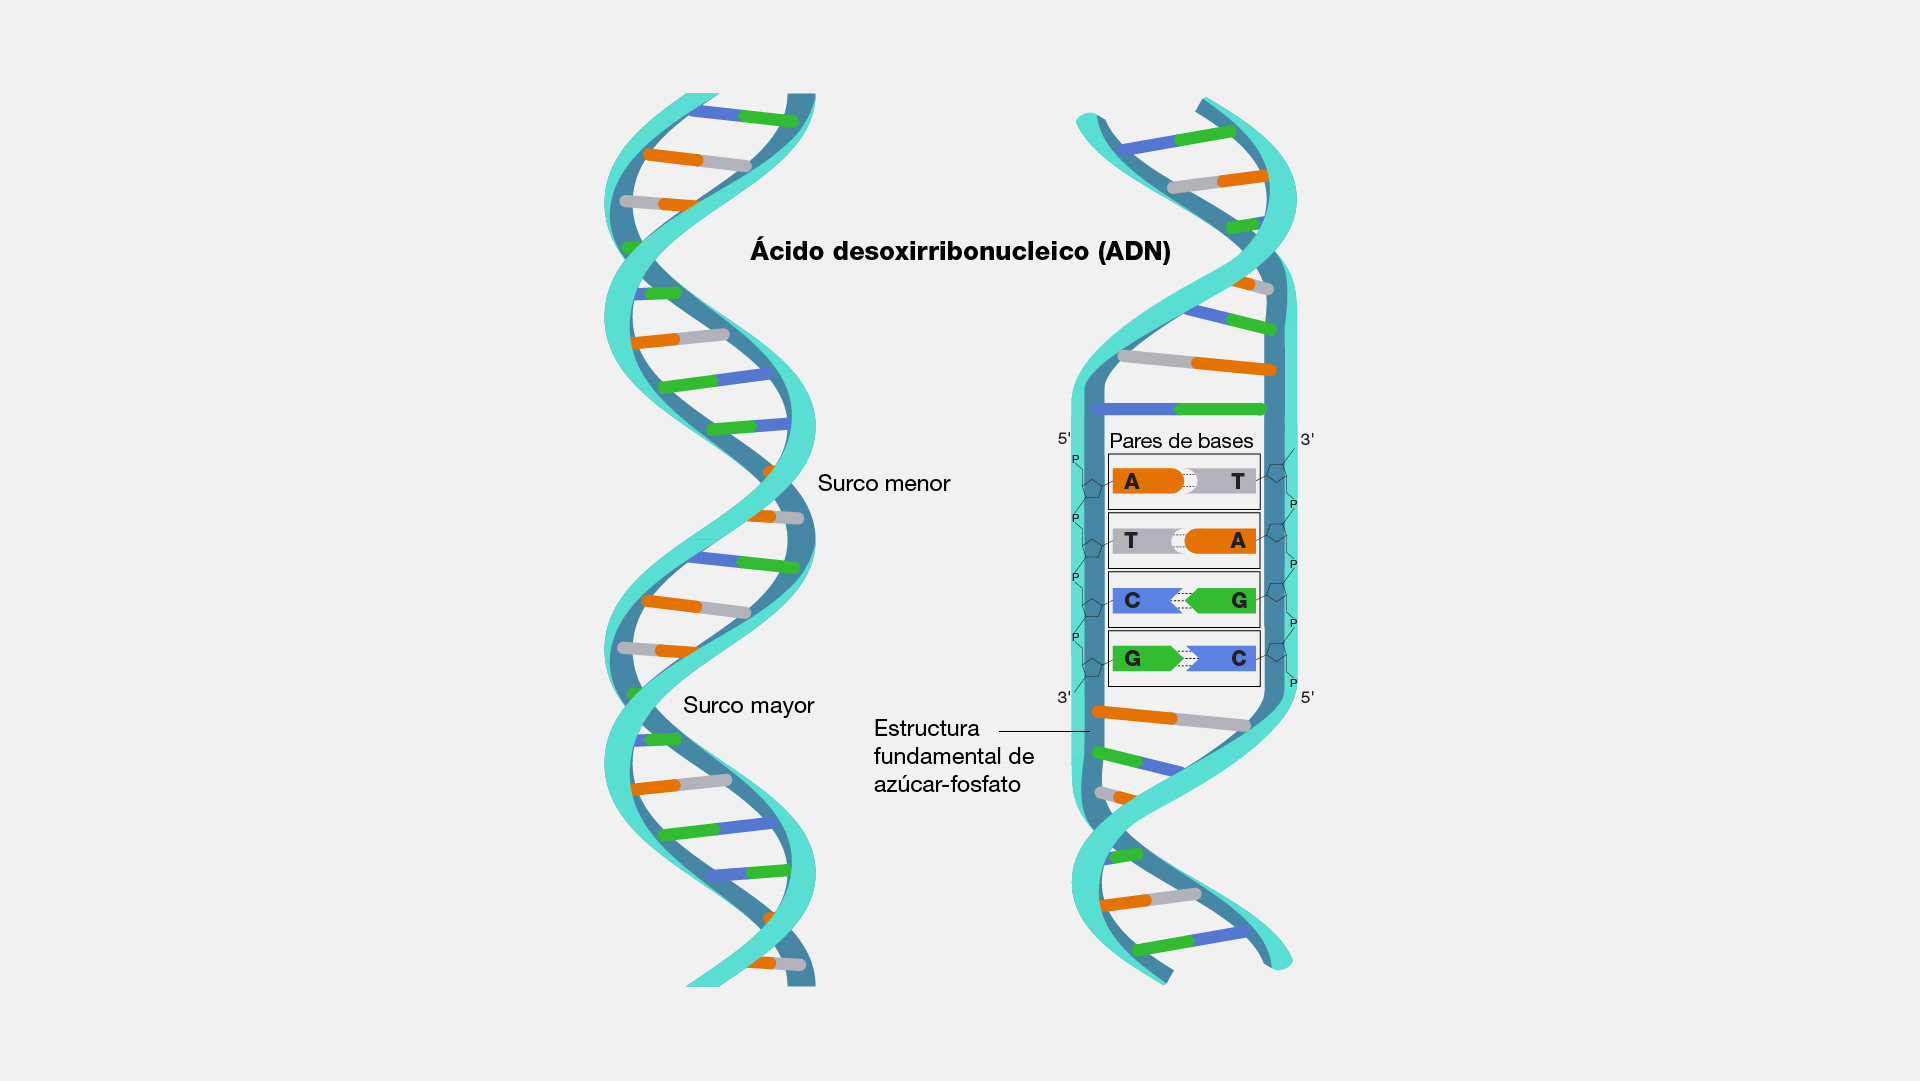
\includegraphics[width=\textwidth]{img/Estructura_del_ADN.jpg}
    \caption{Estructura del ADN \cite{genome}}
\end{figure}

La secuencia que constituye la sucesión de bases en una de las cadenas de ADN representa la información genética codificada en dicha cadena. Por la complementariedad de las cadenas, a partir de una de ellas se puede también determinar la información de la otra. Además, cada cadena tiene definida una dirección espacial contraria a la otra, de modo que sólo podemos interpretar una cadena en la dirección correspondiente.

A nivel celular, el ADN se organiza en cromosomas, cada uno de los cuales contiene ADN superenrollado que puede tener cientos de millones de pares de bases. La mayoría de las células humanas contienen 23 pares de cromosomas, uno heredado del padre y el otro de la madre. Los dos cromosomas de un par son prácticamente idénticos, con la excepción del cromosoma sexual, para el cual existen dos tipos, X e Y. Casi todas las células del cuerpo humano contienen copias idénticas del conjunto completo de 23 pares de cromosomas. El conjunto total de ADN de un organismo se conoce como su genoma, cabe destacar que el genoma humano contiene más de tres mil millones de pares de bases.

Un cromosoma humano está compuesto principalmente por ADN no codificante, cuya función apenas se está empezando a entender. En el ADN se encuentran genes que codifican proteínas. Estos genes representan aproximadamente el $2\%$ del genoma humano, sin embargo, son el foco de atención de los genetistas. Los genes a menudo están organizados en exones, que son secuencias que eventualmente serán utilizadas por la célula, alternado con intrones, que serán descartados en el proceso de codificación. La información de estos genes se transcribirá a ARN (ácido ribonucleico) y en muchos casos, se traducirá a proteínas.

En el proceso de transcripción de un gen a ARN, se utiliza la secuencia de ADN del gen (eliminano los intrones) como plantilla. Al igual que el ADN, el ARN está también compuesto por una serie de nucleótidos, pero con ciertas diferencias: el ARN está formado en general por una única cadena y sustituye la timina ($T$) por el uracilo ($U$). Un caso particular de ARN, el ARNm (ARN mensajero), será finalmente traducido a proteína.

Una proteína está compuesta por una secuencia de $20$ posibles aminoácidos. Cada uno de estos aminoácidos está representado por una o más secuencias de tres nucleótidos de ARN conocidas como codones. La combinación de cuatro posibles nucleótidos en grupos de tres resulta en $4^3=64$ codones, lo que significa que la mayoría de los aminoácidos están codificados por más de un codón. La función de una proteína depende finalmente tanto de su secuencia de aminoácidos como de la estructura tridimensional que ha adquirido de su transformación a partir de un ARNm. 

\section{Software utilizado}
Antes de presentar las aplicaciones de HMM en la biología, presentamos los recursos de software que vamos a utilizar para ilustrar algunos ejemplos. Como recurso principal se van a utilizar dos librerías de Python:
\begin{itemize}
    \item \textbf{NumPy}: es una de las librerías más utilizadas de Python, proporciona la capacidad de tratar elementos matemáticos de forma sencilla y eficiente. En este caso se ha utilizado la versión más reciente hasta el momento, la 1.24.3. Se puede consultar la documentación en \cite{numpy}.
    \item \textbf{hmmlearn}: es una librería de códigos abiertos para Python que implementa modelos de Markov ocultos. Utiliza códigos escritos en C++ para los algoritmos, de forma que son más eficientes que si son implementados directamente en Python. También implementa modelos que no hemos visto en este trabajo. Se ha utilizado para este trabajo la versión 0.3.0. Se puede consultar la documentación en \cite{hmmlearn} y el código en \cite{hmmlearnGithub}
\end{itemize}
A partir de estas herramientas se implementarán archivos de Jupyter Notebook que nos servirán para simular los modelos que presentaremos a continuación. Estos desarrollos se encuentran en \url{https://github.com/vdeq79/TFG/tree/main/src}.

\section{Islas CpG}
En biología computacional, la predicción de genes es un problema en el que se busca identificar regiones codificadoras o genes en un ADN. Puesto que estas regiones poseen ciertas periodicidades y propiedades estadísticas, los HMMs se utilizan para el estudio de este problema. Considerando las estructuras de los genes como estados ocultos y los pares de bases del ADN como observaciones, se puede hacer una predicción de genes aplicando el algoritmo de Viterbi. Este razonamiento es aplicable también a otros problemas de análisis biológico como la búsqueda de regiones funcionales, extracción de patrones, búsqueda de motivos de secuencia e identificación de islas CpG. Este último será el objetivo de nuestro estudio en este apartado \cite{bioStudies}.

Las islas CpG son regiones de ADN con una gran concentración de dinucletidos CpG, que son citosinas ($C$) seguido de guaninas ($G$). Se definen formalmente como regiones de al menos 200 pares de bases con una proporción de $C$ o $G$ superior al $50\%$ y con un ratio CpG de observado/esperado superior al $60\%$. Están íntimamente relacionadas con el inicio de un gen en numerosos genomas de mamíferos, por tanto la presencia de una isla CpG es importante en la predicción de genes. Podemos utilizar HMM para determinar si un fragmento corto de ADN proviene de una isla CpG o para encontrar todas las islas CpG en un segmento largo.

Existen diversos modelos que sirven para este problema, vamos a presentar un modelo casi trivial que consta de $2$ estados (con los símbolos + y - presentando la pertenencia a una isla CpG o no):

\begin{figure}[H]
\centering
\captionsetup{justification=centering}
\begin{tikzpicture}[-latex ,auto , node distance =2.2 cm ,semithick, main/.style = {draw, circle, minimum size=1cm}] 
    \node[rectangle, draw, align=center] (1) {Inicio};
    \node[main] (2) [left of=1, below of=1] {+};
    \node[main] (3) [right of=1, below of=1] {-};
    \node[rectangle, draw, align=center] (4) [below of=2]{$C$ o $G: 0.75$\\$A$ o $T: 0.25$};
    \node[rectangle, draw, align=center] (5) [below of=3]{$C$ o $G: 0.4$\\$A$ o $T: 0.6$};

    \draw (1) -- node[above=0.2cm] {$0.5$} (2);
    \draw (1) -- node[above=0.2cm] {$0.5$} (3);
    \path (2) edge [loop above] node {$0.9$} (2);
    \draw (2.10) -- node[midway] {$0.1$} (3.170);
    \path (3) edge [loop above] node {$0.9$} (3);
    \draw (3. 210) -- node[midway] {$0.1$} (2.330);
    
    \draw (2) -- node[] {} (4);
    \draw (3) -- node[] {} (5);
\end{tikzpicture}
\caption{HMM sencillo para identificar islas CpG. Elaboración propia. Tomada de \cite{bioStudies}.}
\end{figure}

Usando este modelo podemos utilizar el algoritmo de Viterbi para identificar islas CpG. Como ejemplo, consideramos la siguiente secuencia:

\seqsplit{TCTCGCTGCCGCCAACCCTCGGCGCCGTCGGGTTCGCCGCGGCTCTGATAAGTCCCGTTTATGGTACCCGGGCCGATCTCTGGTGGGAATCGGAGACCTGTGTACCCTGACGCATCCGTTTGTGTTCCCTACACGGCCGACGCAGACCGGGCGCGCGGCGCCACCCAACGAAGCCCGGGTATGGCACGTGCCCCAGGCGGTGCCCTACCCGTATTTCGGGACAAGTTCCCGGATCGGGTGAAAGTTAACGGAAGGATGCCAAGCAATAGCGGCCACAGGACCCGCCTGGCGACGCATGGACTGGATCCGGAGGTCTGGCCAACAGTTGATTTCATGGGTTACAGCCCCGGTGTAGATCCCCTCATGGTCTCCCGAACCGATTAGTTTGAAAACTGTATCTCCTGGCCGCCTAACAGGTATAAAGAGCCGGCTCACACTGGGGTGAGGGGGCGCGTGGCCCCCTT}


Para determinar si proviene de una isla CpG aplicamos el algoritmo de Viterbi utilizando funcionalidades de \textbf{hmmlearn}. Obtenemos la siguiente secuencia de estados:

\begin{minted}{python}
#Construimos nuestro modelo
model=hmm.CategoricalHMM(n_components=2, n_features=2)
model.startprob_=np.array([0.5,0.5])
model.transmat_=np.array([[0.9,0.1],[0.1,0.9]])
model.emissionprob_=np.array([[.75, 0.25],[0.4,0.6]])
#Declaramos la secuencia que queremos tratar
sample="TCTCGCTGCCGCCAACCCTCGGCGCCGTCGGGTTCGCCGCGGCTCTGATAAGTCCCGTTTATGGTACCCGGGCCGATCTCTGGTGGGAATCGGAGACCTGTGTACCCTGACGCATCCGTTTGTGTTCCCTACACGGCCGACGCAGACCGGGCGCGCGGCGCCACCCAACGAAGCCCGGGTATGGCACGTGCCCCAGGCGGTGCCCTACCCGTATTTCGGGACAAGTTCCCGGATCGGGTGAAAGTTAACGGAAGGATGCCAAGCAATAGCGGCCACAGGACCCGCCTGGCGACGCATGGACTGGATCCGGAGGTCTGGCCAACAGTTGATTTCATGGGTTACAGCCCCGGTGTAGATCCCCTCATGGTCTCCCGAACCGATTAGTTTGAAAACTGTATCTCCTGGCCGCCTAACAGGTATAAAGAGCCGGCTCACACTGGGGTGAGGGGGCGCGTGGCCCCCTT"
#Consideramos una emisión como la presencia de C o G y otra la presencia de A o T
sample_sym=np.array([[0 if letter == 'C' or letter == 'G' else 1] for letter in sample])
log_prob, result=model.decode(sample_sym)
#Tranformamos la salida a los estados
result_sym=np.array(['+' if state==0 else '-' for state in result])
print("".join(result_sym))
>> +++++++++++++++++++++++++++++++++++++++++++-----------------------+++++++++++++++++++++++++++++++++++++++++++++++++++++++++++++++++++++++++++++++++++++++++++++++++++++++++++++++++++++++++++++++++++++++++++++++++---------------------------------------------------------++++++++++++++++++++++++++++++++++++++++++++++++++++-----------------------++++++++++++++++++++++++++++++++++++---------------------++++++++++---------------+++++++++++++++++++++++++++++++++++++++

\end{minted}

Podemos usar este resultado para distinguir los estados correspondientes en la secuencia de observaciones:

\textcolor{blue}{\seqsplit{TCTCGCTGCCGCCAACCCTCGGCGCCGTCGGGTTCGCCGCGGC}}\textcolor{red}{\seqsplit{TCTGATAAGTCCCGTTTATGGTA}}\textcolor{blue}{\seqsplit{CCCGGGCCGATCTCTGGTGGGAATCGGAGACCTGTGTACCCTGACGCATCCGTTTGTGTTCCCTACACGGCCGACGCAGACCGGGCGCGCGGCGCCACCCAACGAAGCCCGGGTATGGCACGTGCCCCAGGCGGTGCCCTACCCG}}\textcolor{red}{\seqsplit{TATTTCGGGACAAGTTCCCGGATCGGGTGAAAGTTAACGGAAGGATGCCAAGCAATA}}\textcolor{blue}{\seqsplit{GCGGCCACAGGACCCGCCTGGCGACGCATGGACTGGATCCGGAGGTCTGGCC}}\textcolor{red}{\seqsplit{AACAGTTGATTTCATGGGTTACA}}\textcolor{blue}{\seqsplit{GCCCCGGTGTAGATCCCCTCATGGTCTCCCGAACCG}}\textcolor{red}{\seqsplit{ATTAGTTTGAAAACTGTATCT}}\textcolor{blue}{\seqsplit{CCTGGCCGCC}}\textcolor{red}{\seqsplit{TAACAGGTATAAAGA}}\textcolor{blue}{\seqsplit{GCCGGCTCACACTGGGGTGAGGGGGCGCGTGGCCCCCTT}}

Donde el color azul representa que las letras provienen de un estado + y el color rojo representa que provienen de un estado - como resultado de aplicar el algoritmo de Viterbi. Si analizamos las secuencias en rojo, podemos ver que contienen una proporción de $T$ o $A$ superior al $50\%$. Pero en definitiva, tenemos una mayor proporción de estados + en la secuencia de estados resultante, lo que sugiere que la secuencia de observaciones puede provenir de una isla CpG.

\section{Alineamiento de pares de secuencias}
En análisis de secuencias, muchas veces es importante comparar dos secuencias para determinar si están funcionalmente relacionadas. Por ejemplo, genes con funciones similares en diferentes organismos suelen tener secuencias de ADN muy parecidas. Si un gen nuevo es suficientemente similar a otro gen de otro organismo cuya función es conocida, entonces es razonable esperar que el nuevo gen ejerza la misma función. Lo mismo ocurre con las proteínas, si se descubre una nueva proteína de la que se desconoce su estructura tridimensional pero con una similitud sustancial entre su secuencia de aminoácidos y la secuencia de una proteína de la que sí se conoce la estructura tridimensional, entonces es razonable esperar que la estructura de la nueva proteína sea de alguna forma similar a la de la proteína conocida.

Para estudiar este problema, comenzamos estableciendo algunas notaciones. Vamos a considerar un par de secuencias, $x$ e $y$ de longitudes $n$ y $m$ respectivamente. Sea $x_i$ el $i$-ésimo símbolo de $x$ e $y_j$ el $j$-ésimo símbolo de $y$, estos símbolos pertenecen a un cierto alfabeto $\mathcal{A}$ que, en el caso del ADN, serán las $4$ bases $\{A,C,G,T\}$ y, en el caso de las proteínas, serán los $20$ aminoácidos.

Si sólo consideramos las secuencias originales el problema sería trivial: sólo existe un único alineamiento en el caso de que $n=m$ y en otro caso, el problema se reduciría en encontrar la mejor posición para incluir una secuencia en otra. El problema real tiene en cuenta posibles inserciones de huecos (\textit{gaps}) en cualquiera de las dos secuencias para obtener alineamientos entre símbolos iguales. No permitiendo insertar hueco en ambas secuencias al mismo tiempo ni insertar dos huecos en diferentes secuencias de forma seguida. 

Estas consideraciones surgen debido a que, al comparar dos secuencias, buscamos evidencias que provengan de un ancestro común a través de un proceso de mutación y selección. Las mutaciones que se tienen en cuenta incluyen sustituciones, que modifican elementos de una secuencia, así como inserciones y eliminaciones, que agregan o eliminan elementos. A continuación, consideremos el siguiente ejemplo:

\begin{exampleth} \label{alineamientoPar}
    Tomamos dos secuencias de ADN:
    \begin{center}
        $x=CACGAAT$, $y=AGTTCAA$
    \end{center}
    Podemos considerar un alineamiento entre estas dos secuencias como sigue:
    \[\begin{array}{c c c c c c c c c c}
        C & A & - & - & - & C & G & A & A & T \\
        - & A & G & T & T & C & - & A & A & -
    \end{array}\]
    donde cada $-$ representa un hueco.
\end{exampleth}

Como podemos apreciar en el ejemplo, las inserciones producen nuevos alineamientos a tener en cuenta. Para valorar estos alineamientos, se define una matriz de puntuaciones que asigna para cada alineamiento de símbolos un valor. Esta matriz se conoce usualmente como la matriz de sustitución. Un ejemplo de matriz de sustitución para secuencias de ADN podría ser la siguiente:
\[\tag{4.\arabic{Bio}} \label{matrizSustitución}
S=\begin{blockarray}{ccccc}
 & A & C & G & T \\
\begin{block}{c(cccc)}
  A & 10 & -3 & -2 & 1 \\
  C & -2 & 8 & 1 & -2 \\
  G & -3 & 1 & 9 & -3 \\
  T & 0 & -3 & -2 & 6\\
\end{block}
\end{blockarray}
 \]
En esta matriz, cada elemento representa la puntuación que obtendría un alineamiento entre el símbolo de la fila y el símbolo de la columna. Cada uno de estos valores, se puede calcular de la siguiente manera:
\[s(a,b)=\log\left(\dfrac{p_{ab}}{q_a\cdot q_b}\right)\]
siendo $a$ y $b$ elementos del alfabeto $\mathcal{A}$, $p_{ab}$ la probabilidad de que se produzca un emparejamiento entre $a$ y $b$ y $q_a$ la frecuencia relativa esperada de que se produzca un símbolo $a$ en una secuencia. 

Estos valores son relevantes pues afectan a la significación final del análisis: si tenemos un sistema de puntuación ajustado a la realidad, podremos afirmar con mayor seguridad las similitudes entre dos secuencias. Por esta razón, existen métodos para derivar estos valores a partir de datos conocidos y matrices de sustitución utilizadas ampliamente como las matrices PAM o BLOSUM.

Además de los alineamientos entre los símbolos del alfabeto, se tienen en cuenta también los alineamientos entre un símbolo y un hueco. Estos alineamientos tienen una puntuación negativa, lo que se conoce generalmente como penalizaciones por hueco (\textit{gap penalties}). El coste asociado a una consecución de huecos de longitud $g$ suele venir dado por una de las dos siguientes funciones:
\[\gamma_1(g)=-gd,\]
\[\gamma_2(g)=-d-(g-1)e,\]
donde $d$ se considera la penalización por iniciar la secuencia de huecos y $e$ se considera la penalización por extender la secuencia, usualmente con un valor menor que $d$. Mientras que en $\gamma_1$ se tratan todos los huecos por igual, en $\gamma_2$ se penalizan menos las secuencias de huecos con mayores longitudes. Esto es deseable cuando se prevé que las inserciones de varios huecos sean tan frecuentes como las inserciones de un único hueco. En la práctica, los valores $d$ y $e$ se seleccionan empíricamente una vez elegidos los valores de la matriz de sustitución.

Con estos elementos, podemos determinar el mejor alineamiento con huecos entre dos secuencias entendiéndolo como aquel con mayor puntuación dada la matriz de sustitución. Si consideramos las dos secuencias enteras, estaremos hablando del alineamiento global de pares de secuencias. Si lo que buscamos es el mejor alineamiento entre subsecuencias de $x$ e $y$, entonces estaremos hablando del alineamiento local.

Para nuestro estudio, vamos a centrarnos en el problema de alineamiento global. Este problema se puede resolver empleando el algoritmo de Needleman-Wunsch, un algoritmo de programación dinámica que garantiza encontrar el alineamiento óptimo entre dos secuencias con posibles huecos. Pero también podemos utilizar un tipo específico de HMM para resolver este problema, los \textit{Pair HMMs}.

\subsection{Pair HMM}
A diferencia de los HMMs que habíamos presentado hasta ahora, los \textit{pair HMMs} generan dos salidas en cada estado en lugar de uno. Por esta razón, podemos utilizar este modelo para el problema de alineamiento de pares. Existen distintas variaciones de este modelo, vamos a presentar el modelo ilustrado en \cite{Durbin}. 

%El espacio de salidas del modelo está compuesto por los posibles alineamientos que pueden haber: entre dos símbolos del alfabeto $\mathcal{A}$, entre un símbolo y un hueco o entre un hueco y un símbolo. En definitiva:
%\[\mathbb{V}=\{\mathcal{A}\times\mathcal{A}\}\cup \{\mathcal{A}\times -\} \cup \{-\times\mathcal{A}\} \]

El espacio de estados consiste principalmente en tres estados: en el estado $M$ se generan dos símbolos del alfabeto $\mathcal{A}$ mientras que en los estados $X$ e $Y$ se emite un símbolo de la salida correspondiente dejando un hueco en la otra. Llamaremos $p_{ab}$ a la probabilidad de que se emitan los símbolos $a$ y $b$ desde el estado $M$ y $q_{a}$ la probabilidad de emitir un símbolo $a$ y un hueco desde los estados $X$ e $Y$.

A los estados $X$ e $Y$ se les conoce como estados de inserción (o estado de inserción y eliminación en algunas fuentes, por ejemplo \cite{Marina}) y al estado $M$, el estado de alineamiento (\textit{match state}). Para entender mejor los estados volvemos a tomar el alineamiento del ejemplo \ref{alineamientoPar}, la secuencia de estados que produce dicho alineamiento es la siguiente:

\begin{exampleth}
    \[\begin{array}{c c c c c c c c c c c}
       x \longrightarrow & C & A & - & - & - & C & G & A & A & T \\
       y \longrightarrow & - & A & G & T & T & C & - & A & A & - \\
       \hline 
       \text{Estado} & X & M & Y & Y & Y & M & X & M & M & X 
    \end{array}\]
\end{exampleth}

Asumiendo que las transiciones a los estados de inserción se tratan de forma análoga, existen dos parámetros para definir las probabilidades de transición:
\begin{itemize}
    \item[$\mu=$] probabilidad de pasar del estado $M$ a un estado de inserción ($X$ o $Y$).
    \item[$\epsilon=$] probabilidad de permanecer en un estado de inserción.
\end{itemize}

Puesto que estamos tratando con secuencias espaciales en lugar de temporales, tiene sentido definir un estado de inicio y un estado de fin. Ambos estados son estados silenciosos, estados que no producen ninguna salida. El hecho de añadir un estado de inicio facilita posteriormente la modificación de los algoritmos. Este estado sustituye la función de la distribución inicial, de modo que el modelo siempre empezará por el estado de inicio. Para este problema, podemos considerar que el estado de inicio tiene las mismas probabilidades de transición que $M$.

Por otro lado, al añadir un estado de fin necesitamos introducir un nuevo parámetro, la probabilidad de pasar a dicho estado desde los otros estados. Asumimos que dicha probabilidad es la misma desde cualquiera de los otros estados y la denotamos por $\tau$. Este valor influirá en la longitud media de los alineamientos generados por el modelo. Con estos elementos, tenemos el modelo que se muestra en la figura \ref{pairEjemplo}.

\begin{figure}
\centering
\begin{tikzpicture}[-latex ,auto , node distance =3.5 cm ,semithick, main/.style = {draw, circle, minimum size=1.2cm}] 
    \node[main] (1) {Inicio};
    \node[main] (2) [right of=1] {$M$};
    \node[main] (3) [right of=2, above=1.4 cm of 2] {$X$};
    \node[main] (4) [right of=2, below=1.4 cm of 2] {$Y$};
    \node[main] (5) [right of=3, below = 1.4cm of 3] {Fin};
    
    \path (1) edge [bend left, above, pos=0.7] node {$1-2\mu-\tau$} (2);
    \draw (1) edge [bend left=35] node {$\mu$} (3);
    \draw (1) edge [bend right=40] node {$\mu$} (4);
    \draw (1) edge [bend right=90] node {$\tau$} (5);
    
    \path (2) edge [distance=2cm, out=170, in=210, below, pos=0.7] node {$1-2\mu-\tau$} (2);
    \draw (2) edge [bend left=10] node {$\mu$} (3);
    \draw (2) edge [bend right=10, below] node {$\mu$} (4);
    \draw (2) -- node[midway, below] {$\tau$} (5);

    \path (3) edge [distance=2cm, out=330, in=30, right=1cm] node {$\epsilon$} (3);
    \draw (3) edge [bend left=10] node {$1-\epsilon-\tau$} (2);
    \draw (3) edge [bend right] node {$\tau$} (5);

    \path (4) edge [distance=2cm, out=10, in=70, right=1cm] node {$\epsilon$} (4);
    \draw (4) edge [bend right=10, right=0.1cm] node {$1-\epsilon-\tau$} (2);
    \draw (4) edge [bend right, below] node {$\tau$} (5);

    %\path (5) edge [distance=1cm, above] node {1} (5);
    
\end{tikzpicture}
\caption{Estructura de \textit{pair HMM}. Elaboración propia. Tomada de \cite{Durbin}.}
\label{pairEjemplo}
\end{figure}
Una vez conocido el modelo, podemos aplicar el algoritmo de Viterbi adaptado para encontrar el alineamiento óptimo. En este caso, la entrada consiste en dos secuencias $x=(x_1,\dots,x_n)$ e $y=(y_1,\dots,y_m)$ y la salida es la secuencia de estados que conduce al alineamiento óptimo. 

Utilizaremos los índices $i$ y $j$ para referirnos a los elementos de las secuencias $x$ e $y$. Puesto que $x_i$ e $y_j$ son elementos del alfabeto $\mathcal{A}$, usaremos la notación $p_{x_iy_j},\,q_{x_i},\,q_{y_j}$ para distinguir los alineamientos entre los símbolos y los posibles huecos de $x$ e $y$.

Recordemos que en el algoritmo original:
\[
    \delta_t(i)=\max_{(q_0,q_1\dots,q_{t-1})\in\mathbb{S}^t}P[\mathcal{X}_0^{t}=(q_0,q_1,\dots,q_{t-1},s_i),\mathcal{Y}_0^t=(O_0,\dots,O_t)].
\]

Y se calcula de la siguiente forma:
\begin{align*}
    &\delta_0(i)=b_{s_i}(O_0)\cdot\pi_i, \\
    &\delta_t(i)=\max_{j=1,\dots,N}\left(a_{ji}\cdot\delta_{t-1}(j)\right) \cdot b_{s_i}(O_t), &&1\leq i\leq N,\quad1\leq t\leq r. \Bioadd\label{viterbiOriginal}
\end{align*}

En este caso, sólo tenemos que calcular las variables relacionadas con los estados $M,\,X$ e $Y$. El estado de inicio se representará también por el estado $M$ por simplicidad. Puesto que el estado fin es un estado silencioso y representa el final del alineamiento, tendrá un tratamiento especial. 

Usando los índices $i$ y $j$, la variable del algoritmo de Viterbi pasa a ser de forma $\delta_{i,j}(s)$ con $s\in\{M,X,Y\}$. Esta variable tiene el mismo significado que en el caso general: es la probabilidad de la secuencia de estados más probable terminado en el estado $s$, habiendo considerado hasta las posiciones $i$ y $j$ de las secuencias de entrada. Por lo tanto, el cálculo es idéntico al caso general, sustituyendo el índice temporal por los índices $i$ y $j$.

Concretamente, inicializamos el algoritmo asignando los siguientes valores:
\[\delta_{0,0}(M)=1.\]
\[\delta_{0,j}(X)=\delta_{i,0}(Y)=0,\qquad  0\leq i\leq n, \, 0\leq j \leq m.\]
\[\delta_{0,j}(M)=\delta_{i,0}(M)=0,\qquad  1\leq i\leq n, \, 1\leq j \leq m.\]


El primer caso se debe a que siempre empezamos en el estado de inicio (que hemos representado en este caso por el estado $M$) y al ser silencioso podemos asumir que tiene la probabilidad de emisión $1$. Los otros casos se deben a que son situaciones imposibles. Por ejemplo, $\delta_{0,1}(X)$ es la probabilidad de que se haya considerado $y_1$ y ningún símbolo de $x$ habiendo tomado como último estado el estado $X$. Esto contradice con la propia definición de $X$, pues en dicho estado siempre se emite un símbolo de $x$ con un hueco en $y$.

El resto de las variables se calculan de forma similar que en \eqref{viterbiOriginal}, iremos por casos:
\begin{itemize}
    \item $\delta_{i,j}(M)$ indica que se ha alineado $x_i$ e $y_j$ tomando como último estado el estado $M$. Además, aplicando recursividad, tenemos que encontrar la probabilidad de la secuencia más probable habiendo considerado hasta las posiciones $i-1$ y $j-1$ terminado en un estado $s$ y considerar la transición de $s$ a $M$:
    \[\delta_{i,j}(M)=p_{x_iy_j}\cdot \max
    \begin{cases}
        (1-2\mu-\tau)\cdot\delta_{i-1,j-1}(M) \\
        (1-\epsilon-\tau)\cdot\delta_{i-1,j-1}(X) \\
        (1-\epsilon-\tau)\cdot\delta_{i-1,j-1}(Y)
    \end{cases} \quad 1\leq i\leq n, \, 1\leq j \leq m.\] 

    \item $\delta_{i,j}(X)$ indica que se ha emitido $x_i$ y un hueco tomando como último estado el estado $X$. Puesto que en este caso no se emite ningún símbolo de $y$, quiere decir que $y_j$ ya había sido emitido anteriormente. Como no es posible pasar del estado $Y$ al $X$, existen dos posibilidades: el alineamiento entre $x_{i-1}$ e $y_j$ o el alineamiento entre $x_k$ e $y_j$ con $k<i-1$. Este último caso implicaría la emisión de $x_{i-1}$ con un hueco, por lo tanto:
    \[\delta_{i,j}(X)=q_{x_i}\cdot \max 
    \begin{cases}
        \mu\cdot\delta_{i-1,j}(M) \\
        \epsilon\cdot\delta_{i-1,j}(X) 
    \end{cases} \qquad 1\leq i\leq n, \, 0\leq j \leq m.\]

    \item $\delta_{i,j}(Y)$ se calcula de mismo modo que $\delta_{i,j}(X)$:
    \[\delta_{i,j}(Y)=q_{y_j}\cdot \max 
    \begin{cases}
        \mu\cdot\delta_{i,j-1}(M) \\
        \epsilon\cdot\delta_{i,j-1}(Y) 
    \end{cases} \qquad 0\leq i\leq n, \, 1\leq j \leq m.\]
\end{itemize}
Finalmente, se calcula:
\[\delta(Fin)=\tau\cdot\max\{\delta_{n,m}(M),\,\delta_{n,m}(X),\,\delta_{n,m}(Y)\}.\]
Para obtener la secuencia óptima mantenemos el estado correspondiente al argumento máximo de cada variable y lo recuperamos desde $\delta(Fin)$ del mismo modo que en el algoritmo original. Para evitar el problema de convergencia a $0$, basta aplicar logaritmo a las variables tal como hacíamos en la versión original.

Una de las ventajas que nos proporciona la utilización de \textit{pair HMM} respecto a algoritmos que emplean directamente programación dinámica, es que ahora podemos calcular la probabilidad de que dos secuencias estén relacionadas según el modelo, independientemente del alineamiento. Lo hacemos considerando todos los posibles alineamientos:
\[P[x,y]=\sum_{Alineamiento\, Q}P[x,y,Q].\]
Para calcular esta suma adaptamos el algoritmo de avance a este modelo. La variable de avance se puede calcular de forma recursiva similar a la variable de Viterbi, pero sumando las variables previas en lugar de calcular el máximo. Una vez obtenida esta probabilidad, podemos calcular la probabilidad del alineamiento óptimo $Q^*$. Por la definición de la variable de Viterbi:
\[P[Q^*|x,y]=\dfrac{P[Q^*, x,y]}{P[x,y]}=\dfrac{\delta(Fin)}{P[x,y]}\,.\]
Para evitar el problema de convergencia a $0$ en el algoritmo de avance, podemos tomar logaritmo de las variables. Recordemos que:
\begin{equation*}
        \alpha_{t+1}(j)=\left(\sum_{i=1}^N\alpha_{t}(i)\cdot a_{ij}\right)\cdot b_{s_j}(O_{t+1}), \qquad 0\leq t\leq r-1 , \quad 1\leq j\leq N.
\end{equation*}
Aplicando logaritmo:
\begin{align*}
    \log(\alpha_{t+1}(j)) &= \log\left(\sum_{i=1}^N\alpha_{t}(i)\cdot a_{ij}\right) + \log(b_{s_j}(O_{t+1})) \\
        &=\log\left(\sum_{i=1}^N\exp\left[\log(\alpha_{t}(i))+\log(a_{ij})\right]\right) + \log(b_{s_j}(O_{t+1}))
\end{align*}
Utilizando la función \textbf{logsumexp} de la librería \textbf{SciPy}\cite{scipy}, podemos calcular fácilmente este logaritmo.

\begin{exampleth}
Utilizando las librerías \textbf{hmmlearn} y \textbf{NumPy} se ha implementado la clase \textbf{PairHMM} en python. Esta clase tiene la misma estructura que hemos explicado anteriormente y también se ha implementado el algoritmo de Viterbi y el algoritmo de avance correspondiente. A continuación, vamos a alinear las secuencias del ejemplo \ref{alineamientoPar} utilizando esta clase con los siguientes parámetros:
\[\mu=0.2 \qquad \epsilon=0.3 \qquad \tau=0.1\]
\[p_{AA}=p_{CC}=p_{GG}=p_{TT}=0.2\]
\[p_{AT}=p_{TA}=p_{CG}=p_{GC}=0.025\]
\[p_{AC}=p_{AG}=p_{CA}=p_{CT}=p_{GA}=p_{GT}=p_{TC}=p_{TG}=0.0125\]
\[q_A=q_C=q_G=q_T=0.25\]

Tomando las secuencias $x=CACGAAT$ e $y=AGTTCAA$, aplicamos el algoritmo de Viterbi respecto del modelo que construimos con los anteriores parámetros:

\begin{minted}{python}
model = PairHMM(alphabet=["A", "C", "G", "T"], mu=0.2, epsilon=0.5, tau=0.1, match_probabilities=[0.2, 0.0125, 0.0125, 0.025, 0.0125, 0.2, 0.025, 0.0125, 0.0125, 0.025, 0.2, 0.0125, 0.025, 0.0125, 0.0125, 0.2], insert_probabilities=[0.25]*4)
x="CACGAAT"
y="AGTTCAA"
sequence, alignment, p_fin=model.modifiedViterbi( x, y )
print("\n".join(alignment))
>> CA---CGAAT
>> -AGTTC-AA-
\end{minted}

Como se puede apreciar, nos devuelve el siguiente alineamiento:
    \[\begin{array}{c c c c c c c c c c}
        C & A & -& -& -& C& G& A& A& T \\
        -& A& G& T& T& C& -& A& A& -
    \end{array}\]
Este es el mismo alineamiento que vimos en el ejemplo \ref{alineamientoPar}, pero no se trata de una casualidad pues dicho alineamiento es el mejor alineamiento con la matriz de sustitución dada en \eqref{matrizSustitución} y usando la función de penalización de huecos $\gamma(g)=-g$ \cite{Vidyasagar}.

Observando esa matriz podemos ver que, aparte de los alineamientos entre los mismos símbolos, los alineamientos entre $A$ con $T$ y $C$ con $G$ se valoran también positivamente, lo que se traduce en una mayor probabilidad que el resto. 

Calculamos la probabilidad de que $x$ e $y$ estén relacionados independientemente del alineamiento:
\begin{minted}{python}
total_prob=model.modifiedFoward(x, y)
print(total_prob)
>> 5.85602525347472e-12
\end{minted}

Esta probabilidad nos puede parecer baja, pero si calculamos esta probabilidad con dos secuencias idénticas bajo el mismo modelo:
\begin{minted}{python}
print(model.modifiedFoward("AAAAAAA", "AAAAAAA"))
>> 2.8039432167959317e-08
\end{minted}

Podemos apreciar que esta probabilidad es en general baja y disminuye significativamente conforme aumenta la longitud de las secuencias. Calculamos ahora la probabilidad del alineamiento óptimo:
\begin{minted}{python}
p_sequence = p_fin/total_prob
print(p_sequence)
>> 0.10373930673190596
\end{minted}
En este caso, obtenemos un valor bastante significativo, lo cual nos indica la \enquote{correctitud} del alineamiento. En general, la probabilidad del alineamiento óptimo suele ser un valor extremadamente pequeño debido a que existen numerosos alineamientos muy similares al óptimo que tienen una probabilidad ligeramente menor.

Finalmente, cabe enfatizar que el alineamiento que nos proporciona el algoritmo de Viterbi depende de los parámetros, un cambio como el de modificar el valor de $\epsilon$ a $\epsilon=0.5$ produce un alineamiento diferente:

\begin{minted}{python}
model = PairHMM(alphabet=["A", "C", "G", "T"], mu=0.2, epsilon=0.5, tau=0.1, match_probabilities=[0.2, 0.0125, 0.0125, 0.025, 0.0125, 0.2, 0.025, 0.0125, 0.0125, 0.025, 0.2, 0.0125, 0.025, 0.0125, 0.0125, 0.2], insert_probabilities=[0.25]*4)
x="CACGAAT"
y="AGTTCAA"
sequence, alignment, p_fin=model.modifiedViterbi( x, y )
print("\n".join(alignment))

>> CACG---AAT
>> -A-GTTCAA-
\end{minted}
\end{exampleth}

\section{Profile HMM}
En el apartado anterior hemos visto cómo podemos alinear dos secuencias de ADN o de proteínas para determinar si están relacionadas. En general, secuencias biológicas con funciones similares forman familias. Para caracterizar las propiedades de una familia, se acude al alineamiento múltiple de secuencias de la familia. Una vez obtenido dicho alineamiento, podemos determinar si una nueva secuencia $x$ pertenece a la familia correspondiente y, en caso afirmativo, concluir que tiene una determinada funcionalidad. 

Para modelar las similitudes resultantes del alineamiento, podemos usar un tipo particular de HMM llamado \textit{profile HMM}. En este apartado, vamos a asumir que tenemos dado el alineamiento múltiple de secuencias de una familia y vamos a presentar la forma de construir el \textit{profile HMM} correspondiente. 

A diferencia de los HMMs generales, los \textit{profile HMMs} tienen una estructura estrictamente lineal y no cíclica. El primer paso para construir el modelo es determinar su longitud. Para ello, necesitamos separar el alineamiento en dos posibles regiones: la región de alineamiento, que está formada por posiciones cuyos elementos son mayoritariamente símbolos y la región de inserción formada por posiciones con una alta frecuencia de huecos. Aunque existen diferentes criterios, lo usual es que posiciones cuyos huecos son más de la mitad de los elementos formen parte de la región de inserción y en caso contrario, formen parte de la región de alineamiento. Veamos el siguiente ejemplo:

\begin{exampleth} \label{alineamientoMúltiple}
    \[\begin{array}{c c c c c c}
        T & A & - & -  & T & C \\
        T & A & G & -  & T & C \\
        T & A & G & A  & - & C \\
        - & A & G & -  & T & G \\
        \textcolor{blue}{M} & \textcolor{blue}{M} & \textcolor{blue}{M} & \textcolor{red}{I} & \textcolor{blue}{M} & \textcolor{blue}{M}
    \end{array}\]    
    Las posiciones con \textcolor{blue}{$M$} en última fila indican que pertenecen a la región de alineamiento mientras que la posición con \textcolor{red}{$I$} indica que pertenece a la región de inserción.
\end{exampleth}

Una vez identificadas las regiones, la longitud del modelo viene dada por el número de posiciones que forman parte de la región de alineamiento. Conocida la longitud, el siguiente paso es construir el espacio de estados, que está principalmente constituido por $3$ tipos de estados: los estados de alineamiento $M_k$, los estados de inserción $I_k$ y los estados de eliminación $D_k$. Cada uno de de los índices $k$, corresponde con la $k$-ésima posición dentro de la región de alineamiento comenzando desde $1$. 
Para el ejemplo \ref{alineamientoMúltiple} tenemos:
\[\begin{array}{c c c c c c c}
   & T & A & - & -  & T & C \\
   & T & A & G & -  & T & C \\
   & T & A & G & A  & - & C \\
   & - & A & G & -  & T & G \\
   \hline
  k= & 1 & 2 & 3 & & 4 & 5 
\end{array}\]   
A partir de la longitud $n$, construimos un HMM trivial formado por los estados de alineamiento $M_k$ con $k=1,\dots, n$ y probabilidades de transición $1$ al siguiente estado $M_{k+1}$. Los estados $M_k$ representan el caso de que un símbolo de $x$ se alinee con el símbolo más frecuente de la posición correspondiente. Las probabilidades de emisión de $M_k$ corresponden con las frecuencias relativas de cada símbolo en la posición $k$-ésima del alineamiento. También consideramos los estados de inicio y fin, con los mismos significados que en el caso de \textit{pair HMM} pero con probabilidades de transición triviales. Para el ejemplo \ref{alineamientoMúltiple} tenemos el siguiente HMM:

\begin{figure}[H]
\centering
\begin{tikzpicture}[-latex ,auto, node distance =1.5 cm ,semithick, main/.style = {draw, rectangle, minimum size=0.8cm}] 
    \node[main] (1) {Inicio};
    \node[main] (2) [right of=1] {$M_1$};
    \node[main] (3) [right of=2] {$M_2$};
    \node[main] (4) [right of=3] {$M_3$};
    \node[main] (5) [right of=4] {$M_4$};
    \node[main] (6) [right of=5] {$M_5$};
    \node[main] (7) [right of=6] {Fin};
    
    \draw (1) -- node[] {} (2);
    \draw (2) -- node[] {} (3);
    \draw (3) -- node[] {} (4);
    \draw (4) -- node[] {} (5);
    \draw (5) -- node[] {} (6);
    \draw (6) -- node[] {} (7);

    
\end{tikzpicture}
\caption{HMM trivial a partir del ejemplo \ref{alineamientoMúltiple}.}
\end{figure}

A partir del modelo trivial, añadimos los estados $I_k$ y $D_k$. Los estados $I_k$ modelan las inserciones, emisiones de símbolos adicionales a los $n$ símbolos emitidos por el modelo trivial. En otras palabras, cada inserción representa el alineamiento de un símbolo en una posición fuera de la región de alineamiento y formada mayoritariamente o totalmente por huecos. En este caso, $k$ indica la última posición de la región de alineamiento anterior a la inserción. Para modelar posibles inserciones anteriores a cualquier alineamiento de símbolos, añadimos un estado $I_0$. Cada estado de inserción está asociado a $3$ transiciones posibles: $M_k\rightarrow I_k$ que representa la inserción tras un alineamiento, $I_k\rightarrow I_k$ para permitir inserciones múltiples y la transición $I_k\rightarrow M_{k+1}$ para un nuevo alineamiento. 

Por otra parte, los estados $D_k$ modelan las eliminaciones, emisiones de huecos en la posición $k$ de la región de alineamiento. Cada estado tiene $4$ transiciones posibles: $M_{k-1}\rightarrow D_k$ representando la eliminación en la posición $k$ de la región de alineamiento, $D_k \rightarrow D_{k+1}$ para permitir eliminaciones múltiples, $D_k\rightarrow M_{k+1}$ para alinear después de una eliminación. 

Además, permitimos las transiciones $D_k \rightarrow I_k$ para inserciones tras eliminar e $I_{k}\rightarrow D_{k+1}$ para eliminaciones tras insertar. Estas transiciones son muy poco probables, pero las añadimos pues dejándolas fuera puede generar problemas a la hora de construir el modelo.

Tomando el alineamiento del ejemplo \ref{alineamientoMúltiple}, añadiendo los estados y transiciones al modelo trivial, obtenemos el siguiente \textit{profile HMM}:

\begin{figure}[H]
\centering
    \begin{tikzpicture}[-latex ,auto, node distance =2 cm, semithick, main/.style = {draw, rectangle, minimum size=0.8cm},
        rombo/.style = {draw, diamond, minimum size=0.8cm}, circulo/.style = {draw, circle, minimum size=0.8cm}] 
        \node[main] (1) {Inicio};
        \node[main] (2) [right of=1] {$M_1$};
        \node[main] (3) [right of=2] {$M_2$};
        \node[main] (4) [right of=3] {$M_3$};
        \node[main] (5) [right of=4] {$M_4$};
        \node[main] (6) [right of=5] {$M_5$};
        \node[main] (7) [right of=6] {Fin};
    
        \node[rombo] (8)  [above of=1] {$I_0$};
        \node[rombo] (9) [right of=8] {$I_1$};
        \node[rombo] (10) [right of=9] {$I_2$};
        \node[rombo] (11) [right of=10] {$I_3$};
        \node[rombo] (12) [right of=11] {$I_4$};
        \node[rombo] (13) [right of=12] {$I_5$};

        \node[circulo] (14) [above of=9] {$D_1$};
        \node[circulo] (15) [right of=14] {$D_2$};
        \node[circulo] (16) [right of=15] {$D_3$};
        \node[circulo] (17) [right of=16] {$D_4$};
        \node[circulo] (18) [right of=17] {$D_5$};
        
        \draw (1) -- node {} (2);
        \draw (1) -- node {} (8);
        \draw (1) -- node {} (14);

        
        \draw (2) -- node {} (3);
        \draw (2) -- node {} (9);
        \draw (2) -- node {} (15);


        \draw (3) -- node {} (4);
        \draw (3) -- node {} (10);
        \draw (3) -- node {} (16);

        
        \draw (4) -- node {} (5);
        \draw (4) -- node {} (11);
        \draw (4) -- node {} (17);
        
        \draw (5) -- node {} (6);
        \draw (5) -- node {} (12);
        \draw (5) -- node {} (18);
        
        \draw (6) -- node {} (7);
        \draw (6) -- node {} (13);

        \path (8) edge [distance=0.5cm, out=155, in=205] node {} (8);
        \draw (8) -- node {} (2);
        \draw (8) -- node {} (14);

        
        \path (9) edge [distance=0.5cm, out=155, in=205] node {} (9);
        \draw (9) -- node {} (3);
        \draw (9) -- node {} (15);

        
        \path (10) edge [distance=0.5cm, out=155, in=205] node {} (10);
        \draw (10) -- node {} (4);
        \draw (10) -- node {} (16);

        \path (11) edge [distance=0.5cm, out=155, in=205] node {} (11);
        \draw (11) -- node {} (5);
        \draw (11) -- node {} (17);

        \path (12) edge [distance=0.5cm, out=155, in=205] node {} (12);
        \draw (12) -- node {} (6);
        \draw (12) -- node {} (18);

        \path (13) edge [distance=0.5cm, out=155, in=205] node {} (13);
        \draw (13) -- node {} (7);

        \draw (14) -- node {} (15);
        \draw (14) -- node {} (9);
        \draw (14) -- node {} (3);
        
        \draw (15) -- node {} (16);
        \draw (15) -- node {} (10);
        \draw (15) -- node {} (4);

        \draw (16) -- node {} (17);
        \draw (16) -- node {} (11);
        \draw (16) -- node {} (5);
        
        \draw (17) -- node {} (18);
        \draw (17) -- node {} (12);
        \draw (17) -- node {} (6);
        
        \draw (18) -- node {} (7);
        \draw (18) -- node {} (13);
    \end{tikzpicture}
\caption{\textit{Profile HMM} a partir del ejemplo \ref{alineamientoMúltiple}. Elaboración propia.}
\label{profileHMMFinal}
\end{figure}

Determinada la estructura del modelo, ahora necesitamos hallar las probabilidades de transición y de emisión. Con los estados que hemos definido, conocemos para cada una de las secuencias del alineamiento múltiple, la secuencia de estados que la produce. Por lo tanto, podemos estimar las probabilidades contando las transiciones y las emisiones de símbolos de todas las secuencias de estados y calcular las frecuencias relativas correspondientes. Para permitir probabilidades de transición o de emisión que no han sido observadas en el alineamiento original, añadimos un valor ponderado denominado pseudoconteo a los recuentos para evitar probabilidades iguales a cero. Este valor depende de la probabilidad que estamos calculando y del conocimiento que tenemos sobre el problema; el más simple posible es añadir $1$ a todas las observaciones. Veamos a continuación un ejemplo utilizando esta aproximación:

\begin{exampleth}
    Volvemos a tomar el alineamiento múltiple del ejemplo \ref{alineamientoMúltiple} con el modelo correspondiente a la figura \ref{profileHMMFinal}. En primer lugar vamos a determinar los estados que generan cada secuencia. Para evitar confusiones, pondremos $M_0$ para representar al inicio y $M_6$ para representar al fin. 
    \[\begin{array}{c c c c c c c c c}
       & T & A & - & -  & T & C & \implies &  M_0\, M_1\, M_2\,  D_3\,  M_4\,  M_5\,  M_6 \\
       & T & A & G & -  & T & C & \implies &  M_0\,  M_1\,  M_2\,  M_3\,  M_4\,  M_5\,  M_6 \\
       & T & A & G & A  & - & C & \implies &  M_0\,  M_1\,  M_2\,  M_3\,  I_3\,  D_4\,  M_5\,  M_6 \\
       & - & A & G & -  & T & G & \implies &  M_0 \,  D_1 \,  M_2 \,  M_3\,  M_4 \,  M_5 \,  M_6  \\
       \hline
       k= & 1 & 2 & 3 & & 4 & 5 & &
   \end{array}\]   
    Contamos ahora las frecuencias de cada símbolo en los estados $M_k$ e $I_k$, no es necesario calcular para los $D_k$ pues siempre emiten un hueco.

\begin{table}[H]
    \begin{minipage}{.5\linewidth}
        \centering
        \begin{tabular}{|c | C | C | C | C|}
             \hline
             & A & C & G & T \\
             \hline
             $M_1$ & 0 & 0 & 0 & 3 \\
             \hline
             $M_2$ & 4 & 0 & 0 & 0 \\
             \hline
             $M_3$ & 0 & 0 & 3 & 0 \\ 
             \hline
             $M_4$ & 0 & 0 & 0 & 3 \\
             \hline
             $M_5$ & 0 & 3 & 1 & 0 \\
             \hline
        \end{tabular}
        \caption{Emisiones desde $M_k$}
    \end{minipage}%
    \begin{minipage}{.5\linewidth}
        \centering
        \begin{tabular}{|c | C | C | C | C|}
            \hline
            & A & C & G & T \\
            \hline
            $I_0$ & 0 & 0 & 0 & 0 \\
            \hline
            $I_1$ & 0 & 0 & 0 & 0 \\
            \hline
            $I_2$ & 0 & 0 & 0 & 0 \\
            \hline
            $I_3$ & 1 & 0 & 0 & 0 \\ 
            \hline
            $I_4$ & 0 & 0 & 0 & 0 \\
            \hline
            $I_5$ & 0 & 0 & 0 & 0 \\
            \hline
        \end{tabular}
        \caption{Emisiones desde $I_k$}
    \end{minipage}
\end{table}
Para las transiciones entre estados, tenemos las siguientes frecuencias donde cada $k$ representa el índice del estado que inicia la transición:
\begin{table}[H]
    \centering
    \begin{tabular}{|c|C|C|C|C|C|C|C|}
        \hline
        $k$ & 0 & 1 & 2 & 3 & 4 & 5  \\
        \hline
        $M\rightarrow M$ & 3 & 3 & 3 & 2 & 3 & 4\\
        $M\rightarrow D$ & 1 & 0 & 1 & 0 & 0 & - \\
        $M\rightarrow I$ & 0 & 0 & 0 & 1 & 0 & 0 \\
        \hline
        $I\rightarrow M$ & 0 & 0 & 0 & 0 & 0 & 0 \\
        $I\rightarrow D$ & 0 & 0 & 0 & 1 & 0 & - \\
        $I\rightarrow I$ & 0 & 0 & 0 & 0 & 0 & 0 \\
        \hline
        $D\rightarrow M$ & - & 1 & 0 & 1 & 1 & 0 \\
        $D\rightarrow D$ & - & 0 & 0 & 0 & 0 & - \\
        $D\rightarrow I$ & - & 0 & 0 & 0 & 0 & 0 \\
        \hline
    \end{tabular}
    \caption{Frecuencias de transiciones}
\end{table}
Como podemos ver, hay muchas transiciones y emisiones con frecuencia cero, para evitar probabilidades iguales a cero, sumamos $1$ a todas las frecuencias y calculamos las probabilidades:
\begin{table}[H]
    \begin{minipage}{.5\linewidth}
        \centering
        \begin{tabular}{|c | C | C | C | C|}
            \hline
            & A & C & G & T \\
            \hline
            $M_1$ & 1/7 & 1/7 & 1/7 & 4/7 \\
            \hline
            $M_2$ & 5/8 & 1/8 & 1/8 & 1/8 \\
            \hline
            $M_3$ & 1/7 & 1/7 & 4/7 & 1/7 \\ 
            \hline
            $M_4$ & 1/7 & 1/7 & 1/7 & 4/7 \\
            \hline
            $M_5$ & 1/8 & 1/2 & 1/4 & 1/8 \\
            \hline
        \end{tabular}
        \caption{Probabilidades de emisión de $M_k$}
    \end{minipage}%
    \begin{minipage}{.5\linewidth}
        \centering
        \begin{tabular}{|c | C | C | C | C|}
            \hline
            & A & C & G & T \\
            \hline
            $I_0$ & 1/4 & 1/4 & 1/4 & 1/4 \\
            \hline
            $I_1$ & 1/4 & 1/4 & 1/4 & 1/4 \\
            \hline
            $I_2$ & 1/4 & 1/4 & 1/4 & 1/4 \\
            \hline
            $I_3$ & 2/5 & 1/5 & 1/5 & 1/5 \\ 
            \hline
            $I_4$ & 1/4 & 1/4 & 1/4 & 1/4 \\
            \hline
            $I_5$ & 1/4 & 1/4 & 1/4 & 1/4 \\
            \hline
        \end{tabular}
        \caption{Probabilidades de emisión de $I_k$}
    \end{minipage}
\end{table}

\begin{table}[H]
    \centering
    \begin{tabular}{|c|C|C|C|C|C|C|C|}
        \hline
        $k$ & 0 & 1 & 2 & 3 & 4 & 5  \\
        \hline
        $M\rightarrow M$ & 4/7 & 2/3 & 4/7 & 1/2 & 2/3 & 5/6\\
        $M\rightarrow D$ & 2/7 & 1/6 & 2/7 & 1/6 & 1/6 & - \\
        $M\rightarrow I$ & 1/7 & 1/6 & 1/7 & 1/3 & 1/6 & 1/6 \\
        \hline
        $I\rightarrow M$ & 1/3 & 1/3 & 1/3 & 1/4 & 1/3 & 1/2 \\
        $I\rightarrow D$ & 1/3 & 1/3 & 1/3 & 1/2 & 1/3 & - \\
        $I\rightarrow I$ & 1/3 & 1/3 & 1/3 & 1/4 & 1/3 & 1/2 \\
        \hline
        $D\rightarrow M$ & - & 1/2 & 1/3 & 1/2 & 1/2 & 1/2 \\
        $D\rightarrow D$ & - & 1/4 & 1/3 & 1/4 & 1/4 & - \\
        $D\rightarrow I$ & - & 1/4 & 1/3 & 1/4 & 1/4 & 1/2 \\
        \hline
    \end{tabular}
    \caption{Probabilidades de transición}
\end{table}
    
\end{exampleth}

Una vez que conocemos la estructura y la forma de determinar las probabilidades, podemos utilizar el modelo resultante para saber si una secuencia pertenece a una familia. En este caso, el algoritmo de Viterbi y el algoritmo de avance se implementan de forma similar al caso de \textit{pair HMM}. Usando la misma notación definiremos de forma recursiva las variables de Viterbi $\delta_{i}(M_k),\,\delta_{i}(D_k),\,\delta_{i}(I_k)$ con $i\in\{0,\dots,m\}$ siendo $m$ la longitud de la secuencia de entrada $x$. Para inicializar, usamos la notación $M_0$ para el estado de inicio. Puesto que siempre se empieza por dicho estado:
\[\delta_0(M_0)=1\]
Ahora, analizando la figura \ref{profileHMMFinal} tenemos las siguientes relaciones de recursividad:
\begin{itemize}
    \item Puesto que las transiciones a $M_j$ llegan desde estados con índices $j-1$ y desde $M_j$ se emite un símbolo:
    \[\delta_{i}(M_j)=b_{M_j}(x_i)\cdot \max
    \begin{cases}
        a_{M_{j-1}M_j}\cdot\delta_{i-1}(M_{j-1}) \\
        a_{D_{j-1}M_j}\cdot\delta_{i-1}(D_{j-1}) \\
        a_{I_{j-1}M_j}\cdot\delta_{i-1}(I_{j-1})
    \end{cases} \quad 1\leq i\leq m, \, 1\leq j \leq n.\] 

    \item Para permitir emisiones de huecos en la región de alineamiento anterior a cualquier símbolo de $x$, calculamos también $\delta_{0}(D_j)$. Las transiciones a $D_j$ llegan desde estados con índices $j-1$ y desde $D_j$ únicamente se emiten huecos:
    \[\delta_{i}(D_j)=\max
    \begin{cases}
        a_{M_{j-1}D_j}\cdot\delta_{i}(M_{j-1}) \\
        a_{D_{j-1}D_j}\cdot\delta_{i}(D_{j-1}) \\
        a_{I_{j-1}D_j}\cdot\delta_{i}(I_{j-1})
    \end{cases} \quad 0\leq i\leq m, \, 1\leq j \leq n.\] 

    \item Puesto que las transiciones a $I_j$ llegan desde estados con índices $j$ y desde $I_j$ se emite un símbolo:
    \[\delta_{i}(I_j)=b_{I_j}(x_i)\cdot \max
    \begin{cases}
        a_{M_{j}I_j}\cdot\delta_{i-1}(M_{j}) \\
        a_{D_{j}I_j}\cdot\delta_{i-1}(D_{j}) \\
        a_{I_{j}I_j}\cdot\delta_{i-1}(I_{j})
    \end{cases} \quad 1\leq i\leq m, \, 0\leq j \leq n.\] 

\end{itemize}
Para la implementación del algoritmo de avance, basta con sustituir la suma por el máximo en las variables de Viterbi.

\begin{exampleth}
De la misma forma que para \textit{pair HMM} se ha implementado la clase \textbf{ProfileHMM} en Python. Para construir esta clase necesitamos proporcionar el alfabeto correspondiente, el símbolo para el hueco y el alineamiento dado. Utilizando el alineamiento del ejemplo anterior aplicado el pseudoconteo:
\begin{minted}{python}
model = ProfileHMM(alphabet=["A", "C", "G", "T"], gap_symbol='-', alignment=['TA--TC', 'TAG-TC', 'TAGA-C', '-AG-TG'], show_probabilities=True)
>> Probabilidades de emisión de estados de alineamiento:
#Se representa de la misma forma que en el ejemplo anterior.
>> [[0.14285714 0.14285714 0.14285714 0.57142857]
>>  [0.625      0.125      0.125      0.125     ]
>>  [0.14285714 0.14285714 0.57142857 0.14285714]
>>  [0.14285714 0.14285714 0.14285714 0.57142857]
>>  [0.125      0.5        0.25       0.125     ]]
>> Probabilidades de emisión de estados de inserción:
>> [[0.25 0.25 0.25 0.25]
>>  [0.25 0.25 0.25 0.25]
>>  [0.25 0.25 0.25 0.25]
>>  [0.4  0.2  0.2  0.2 ]
>>  [0.25 0.25 0.25 0.25]
>>  [0.25 0.25 0.25 0.25]]
>> Probabilidades de transición entre estados:
#Se representa de la misma forma que en el ejemplo anterior, se ordenan los estados de inicio de transición de forma: M, D, I. No se representan las transiciones al estado fin.
>> [[[0.57142857 0.66666667 0.57142857 0.5        0.66666667]
>>  [0.28571429 0.16666667 0.28571429 0.16666667 0.16666667]
>>  [0.14285714 0.16666667 0.14285714 0.33333333 0.16666667]]
#Transiciones desde los estados de eliminación, ignoraremos la primera columna.
>> [[0.33333333 0.5        0.33333333 0.5        0.5       ]
>>  [0.33333333 0.25       0.33333333 0.25       0.25      ]
>>  [0.33333333 0.25       0.33333333 0.25       0.25      ]]
#Transiciones desde los estados de inserción.
>> [[0.33333333 0.33333333 0.33333333 0.25       0.33333333]
>>  [0.33333333 0.33333333 0.33333333 0.5        0.33333333]
>>  [0.33333333 0.33333333 0.33333333 0.25       0.33333333]]]
>>Probabilidades de transición al estado fin:
#Se ordenan los estados de forma: M, D, I.
>> [[0.83333333 0.16666667]
>>  [0.5        0.5       ]
>>  [0.5        0.5       ]]
\end{minted}
Con este modelo podemos aplicar el algoritmo de Viterbi a una nueva secuencia para obtener un nuevo alineamiento:
\begin{minted}{python}
result, prob = model.modifiedViterbi("ATATGTC")
print(result)
>> ['I', 'M', 'M', 'I', 'M', 'M', 'M']
\end{minted}
Lo que indica que el alineamiento de la nueva secuencia con las secuencias de partida es:
    \[\begin{array}{c c c c c c c c}
        - & T & A & - & - & - & T & C \\
        - & T & A & - & G & - & T & C \\
        - & T & A & - & G & A & - & C \\
        - & - & A & - & G & - & T & G \\
        A & T & A & A & G & - & T & C \\
        \textcolor{red}{I}& \textcolor{blue}{M} & \textcolor{blue}{M} & \textcolor{red}{I} & \textcolor{blue}{M} & & \textcolor{blue}{M} & \textcolor{blue}{M}
    \end{array}\]  
Podemos calcular también la probabilidad de esta secuencia respecto del modelo:
\begin{minted}{python}
total_prob=model.modifiedFoward(x)
print(total_prob)
>> 1.393704882159438e-05
\end{minted}

A continuación vamos a compara dos secuencias cuyas longitudes son menores que $n$:
\begin{minted}{python}
x = "ATC"
result, prob = model.modifiedViterbi(x)
print(result)
>> ['D', 'M', 'D', 'M', 'M']
y = "AAC"
result, prob = model.modifiedViterbi(y)
print(result)
>> ['D', 'M', 'D', 'M', 'M']
\end{minted}
Podemos ver que el algoritmo de Viterbi nos devuelve la misma secuencia de estados. El alineamiento de estas secuencias con las secuencias de partida es:
    \[\begin{array}{c c c c c c}
         T & A & - & - & T & C \\
         T & A & G & - & T & C \\
         T & A & G & A & - & C \\
         - & A & G & - & T & G \\
         - & A & - & - & T & C \\
         - & A & - & - & A & C \\
        \textcolor{blue}{D} & \textcolor{blue}{M} & \textcolor{blue}{D} & & \textcolor{blue}{M} & \textcolor{blue}{M}
    \end{array}\]  
Observando este alineamiento parece lógico suponer que la secuencia $x$ se ajusta más a la familia de partida que $y$. Comprobamos esta intuición aplicamos el algoritmo de avance:
\begin{minted}{python}
total_prob=model.modifiedFoward(x)
print(total_prob)
>> 0.004601382312893029
total_prob=model.modifiedFoward(y)
print(total_prob)
>> 0.003040138977867695
\end{minted}
Puesto que la probabilidad de $x$ es superior a la de $y$, se cumple nuestra suposición.
\end{exampleth}


% Añade sección de referencias al final del documento.
% Selecciona un estilo de cita.
\bibliographystyle{apa-good}
% En research.bib están las entradas de los artículos que citamos.
% Podemos cambiar el nombre del archivo aquí.
\phantomsection
\addcontentsline{toc}{chapter}{Bibliografía}
\bibliography{bib/research}   


\end{document}